\documentclass[twocolumn]{svjour3}          % twocolumn
%DIF LATEXDIFF DIFFERENCE FILE
%DIF DEL gloaguenNmfTraffic_v1.tex   Thu Aug 30 16:25:57 2018
%DIF ADD gloaguenNmfTraffic_v2.tex   Fri Sep 14 14:45:51 2018
%
\smartqed  % flush right qed marks, e.g. at end of proof
%
\usepackage{graphicx}
%
\usepackage{mathptmx}      % use Times fonts if available on your TeX system
%
% insert here the call for the packages your document requires
\usepackage[utf8]{inputenc}
\usepackage[english]{babel}
\usepackage[T1]{fontenc}
\usepackage{layout}

%DIF 15-16c15-16
%DIF < %\usepackage[left,modulo]{lineno}	% numéro de ligne
%DIF < %\linenumbers
%DIF -------
\usepackage[left,modulo]{lineno}	% numéro de ligne %DIF > 
\linenumbers %DIF > 
%DIF -------

%%%%%% SYMBOLES %%%%%
\usepackage{tipa}	% pour avoir l'accent concave
\usepackage{lmodern}	% pour les guillemets
\usepackage{nth}	% pour ^th près des chiffres
\usepackage{nomencl}
\makenomenclature

\renewcommand{\nomname}{List of Abbreviations}

%%%%%% EQUATION %%%%%%
\usepackage{amssymb}
\usepackage{amsmath}
\usepackage{fancybox}
\usepackage{xfrac}	% fraction de type "1/4"
\usepackage{cases}	% système équation
\usepackage[overload]{empheq}
\usepackage{bm}		% pour mettre en gras .
\usepackage{units} 	% x/y barre latérale pour les fractions

%%%%%% FIGURE %%%%%%
\usepackage{graphicx}	% insérer des graphiques
\usepackage{subfig}	% utiliser subfigure
\usepackage{float}	% utiliser H dans les figures
\usepackage[nolists]{endfloat}

%%%%%% TABLEAUX %%%%%%
\usepackage{array,multirow,makecell}
\usepackage[table,xcdraw]{xcolor} % pour avoir des lignes colorées dans les tableau
\usepackage{hhline}	% pour les lignes horizontales
\usepackage{tabularx} % permet itemize dans les cellules
\usepackage{booktabs}

\newcolumntype{L}[1]{>{\raggedright\let\newline\\\arraybackslash\hspace{0pt}}m{#1}}
\newcolumntype{C}[1]{>{\centering\let\newline\\\arraybackslash\hspace{0pt}}m{#1}}
\newcolumntype{R}[1]{>{\raggedleft\let\newline\\\arraybackslash\hspace{0pt}}m{#1}}

%%%%%%%%%%%%%%%%%%%%%
\usepackage[hyphens]{url}	% gérer les adresses www.
\usepackage[hyphenbreaks]{breakurl}

\usepackage[colorlinks,citecolor=black,urlcolor=black,linkcolor=black]{hyperref}  % ps2pdf car je compile via Latex -> dvips -> ps2pdf

% \usepackage{natbib}
\renewcommand{\baselinestretch}{1.025}
%DIF 62a62-63
 %DIF > 
\newcommand{\ml}[1]{\textcolor{red}{ML : #1}} %DIF > 
%DIF -------

\journalname{EURASIP Journal on Audio, Speech and Music Processing}
%DIF PREAMBLE EXTENSION ADDED BY LATEXDIFF
%DIF UNDERLINE PREAMBLE %DIF PREAMBLE
\RequirePackage[normalem]{ulem} %DIF PREAMBLE
\RequirePackage{color}\definecolor{RED}{rgb}{1,0,0}\definecolor{BLUE}{rgb}{0,0,1} %DIF PREAMBLE
\providecommand{\DIFaddtex}[1]{{\protect\color{blue}\uwave{#1}}} %DIF PREAMBLE
\providecommand{\DIFdeltex}[1]{{\protect\color{red}\sout{#1}}}                      %DIF PREAMBLE
%DIF SAFE PREAMBLE %DIF PREAMBLE
\providecommand{\DIFaddbegin}{} %DIF PREAMBLE
\providecommand{\DIFaddend}{} %DIF PREAMBLE
\providecommand{\DIFdelbegin}{} %DIF PREAMBLE
\providecommand{\DIFdelend}{} %DIF PREAMBLE
%DIF FLOATSAFE PREAMBLE %DIF PREAMBLE
\providecommand{\DIFaddFL}[1]{\DIFadd{#1}} %DIF PREAMBLE
\providecommand{\DIFdelFL}[1]{\DIFdel{#1}} %DIF PREAMBLE
\providecommand{\DIFaddbeginFL}{} %DIF PREAMBLE
\providecommand{\DIFaddendFL}{} %DIF PREAMBLE
\providecommand{\DIFdelbeginFL}{} %DIF PREAMBLE
\providecommand{\DIFdelendFL}{} %DIF PREAMBLE
%DIF END PREAMBLE EXTENSION ADDED BY LATEXDIFF
%DIF PREAMBLE EXTENSION ADDED BY LATEXDIFF
%DIF HYPERREF PREAMBLE %DIF PREAMBLE
\providecommand{\DIFadd}[1]{\texorpdfstring{\DIFaddtex{#1}}{#1}} %DIF PREAMBLE
\providecommand{\DIFdel}[1]{\texorpdfstring{\DIFdeltex{#1}}{}} %DIF PREAMBLE
%DIF END PREAMBLE EXTENSION ADDED BY LATEXDIFF

\begin{document}

\title{Estimation of the road traffic sound levels in urban areas based on non-negative matrix factorization techniques}

\author{Jean-R\'emy Gloaguen         \and
		Mathieu Lagrange \and
		Arnaud Can \and
		Jean-Fran\c cois Petiot.}

\institute{J.-R. Gloaguen \at
              Ifsttar Centre de Nantes UMRAE\\
              All\'ee des Ponts et Chauss\'ees 44344 Bouguenais\\
              \email{jean-remy.gloaguen@ifsttar.fr}
\and
			M. Lagrange \at
              LS2N
              1 rue de la Noe 44321 Nantes\\
              \email{mathieu.lagrange@cnrs.fr}
\and
			A.Can \at
              \email{arnaud.can@ifsttar.fr}           \and
			J.-F. Petiot \at
              \email{jean-francois.petiot@ls2n.fr}
}

\date{Received: date / Accepted: date}
% The correct dates will be entered by the editor


\maketitle

\begin{abstract}
The advent of low cost acoustic monitoring devices raises new interesting approaches for improving the monitoring of the acoustic quality of urban areas. State of the art approaches target road traffic noise maps and consider, as input, an estimate of the number and the speed of vehicles in major traffic lanes. Follows a prediction procedure that outputs an acoustic pressure level at any location in the modeled area.

Considering as input the acoustic pressure measured in many locations using a sensor grid approach would greatly complement and improve the quality of the predicted pressure values. Among the technical issues that \DIFdelbegin \DIFdel{raise }\DIFdelend \DIFaddbegin \DIFadd{bring }\DIFaddend this kind of innovative approaches, there is a need to identify which part of the overall acoustic pressure level is due to the road traffic.

In this paper, several techniques based on \DIFaddbegin \DIFadd{the }\DIFaddend non-negative \DIFaddbegin \DIFadd{matrix  }\DIFaddend factorization framework are studied in this application scenario\DIFdelbegin \DIFdel{on a simulated sound scene corpus}\DIFdelend \DIFaddbegin \DIFadd{, on a corpus of simulated sound scenes}\DIFaddend . The task \DIFdelbegin \DIFdel{being }\DIFdelend \DIFaddbegin \DIFadd{is }\DIFaddend to the best of our knowledge never been considered in the literature\DIFdelbegin \DIFdel{, we }\DIFdelend \DIFaddbegin \DIFadd{. We }\DIFaddend propose an experimental protocol to validate the studied approaches that complies with standard reproducible research recommendations. The results show the interest of our proposed approach %DIF > (a NMF based on the adjustment of a learned dictionary directly on the urban sound mixtures)
for such sound environments\DIFdelbegin \DIFdel{as it improves the estimation of the road traffic sound level compared to basic methods.}\DIFdelend \DIFaddbegin \DIFadd{.%DIF >  as it improves the estimation of the road traffic sound level compared to basic methods such as a low-pass filter or supervised NMF.
}\DIFaddend 

\keywords{non-negative matrix factorization \and road traffic sound level \and urban sound environment}
\end{abstract}

\section{Introduction} \label{part:intro}

With the introduction of the European Directive 2002/\-EC/49, cities over 100 000 inhabitants have to produce road traffic noise maps. These maps depict the sound level distribution over the city and an estimation of the number of city dwellers exposed to high noise levels. These maps play both an important communication role and help drawing up action plans to reduce noise exposure. Road traffic noise maps are the result of a simulation process based on the estimation of the traffic density on the main roads and the use of sound propagation modelling. They express as output $L_ {DEN}$ and $L_N$ values, which are \textit{Day-Evening-Night} and \textit{Night} equivalent A-weighted sound levels respectively. \DIFdelbegin \DIFdel{Altough }\DIFdelend \DIFaddbegin \DIFadd{Although }\DIFaddend very useful, the produced noise maps \DIFdelbegin \DIFdel{introduce lot }\DIFdelend \DIFaddbegin \DIFadd{exhibit a large amount }\DIFaddend of uncertainty generated by the numerical tools \cite{van_leeuwen_noise_2015} or by the different calculation methodologies used \cite{leroy_uncertainty_2010}\cite{garg_critical_2014}\DIFdelbegin \DIFdel{, despite the long }\DIFdelend \DIFaddbegin \DIFadd{. It also requires a labor intensive }\DIFaddend data collection and calculation times. \DIFdelbegin \DIFdel{In addition, the usual }\DIFdelend \DIFaddbegin \DIFadd{The result is usually that }\DIFaddend road traffic noise maps are static, aggregating the exposure into indicators $L_{DEN}$ and $L_N$, that ignore the sound levels evolution throughout the day.
The use of acoustic measurements could facilitate their updating or even the generation of dynamic maps \cite{wei_dynamic_2016}. These measurements can be performed at fixed stations spread all over the cities \cite{Mioduszewski} \cite{mietlicki2012innovative}, which would make \DIFdelbegin \DIFdel{available of }\DIFdelend the long-term evolution of the traffic noise \DIFdelbegin \DIFdel{levels}\DIFdelend \DIFaddbegin \DIFadd{available}\DIFaddend . It can also be performed with  mobile stations \cite{can_exploring_2012} \cite{manvell2004sadmam} covering a larger area with fewer sensors but also sparse time periods.

\begin{figure}
[t]
\centering
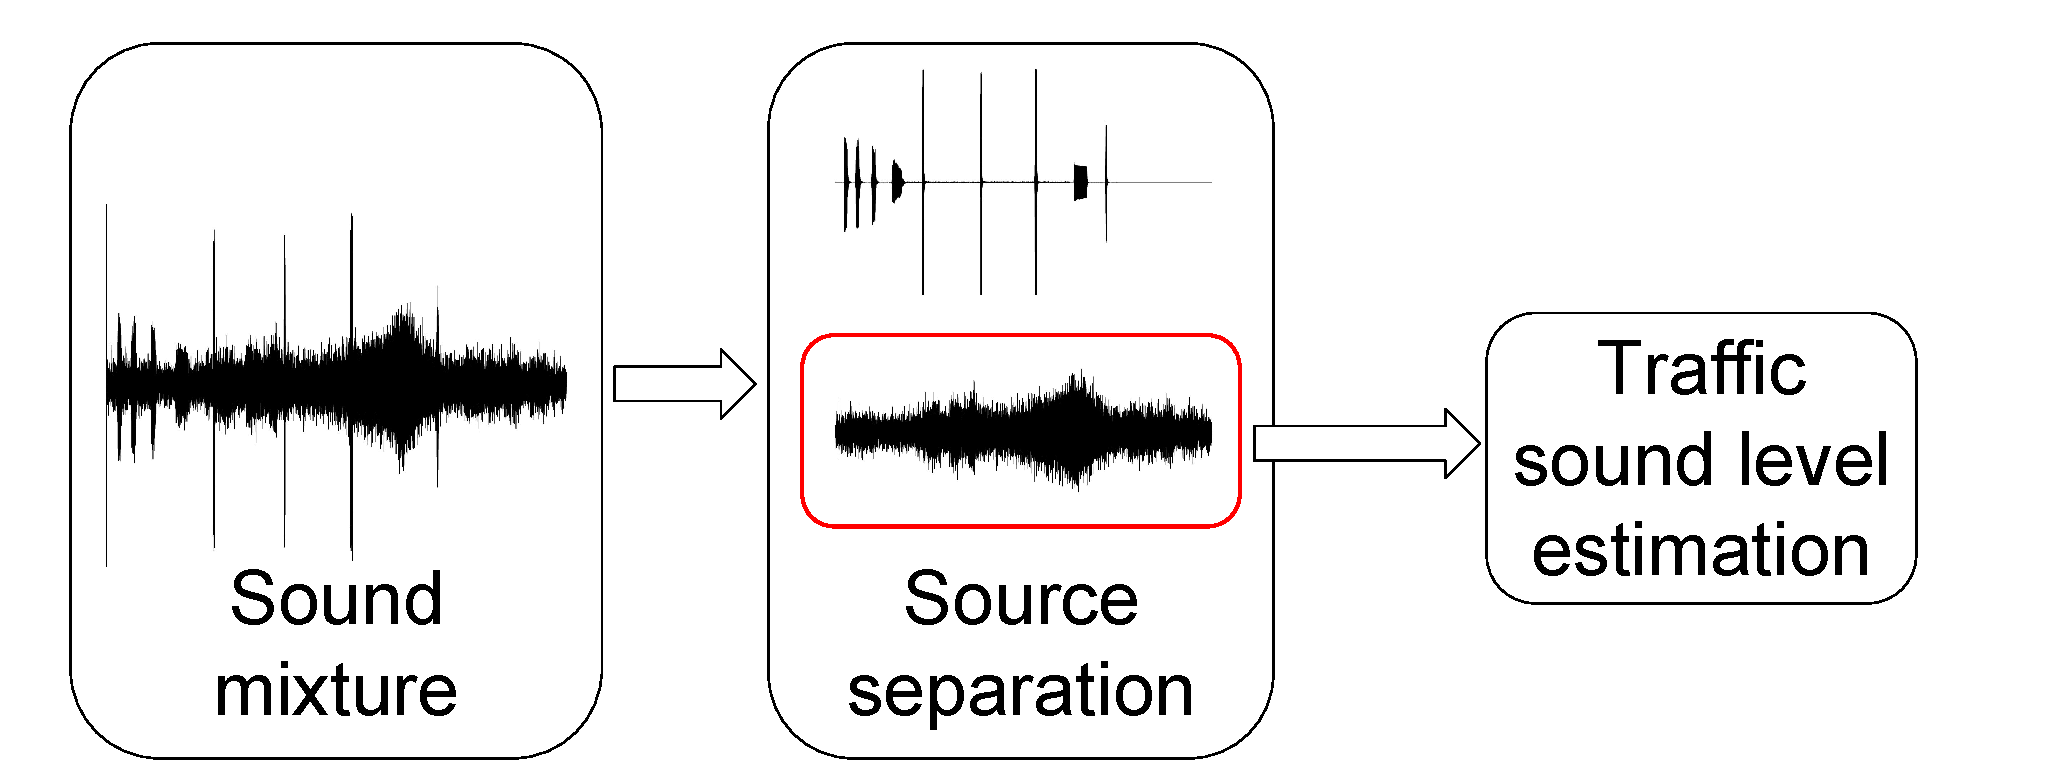
\includegraphics[width=\linewidth]{figures/bloc_diagram_source_separation.pdf}
\caption{Block diagram of the general source separation model.}
\label{fig:diagram}
\end{figure}
Currently, sensor networks in cities are spread for multiple applications (air quality assessment, measurement of meteorological parameters...), including the assessment of urban noise levels. The DYNAMAP project \cite{dynamap_2016} studied the deployment and feasibility of such installations focusing on sensor installations on specific roads at the city scale in Milan and Rome \cite{bellucci_life_2017}.
The SONYC project (Sounds Of New-York City) aims to deploy a sensor network in New-York City for the purpose of monitoring constantly the noise pollution in the city \cite{mydlarz2017implementation}. In order to better know the urban sound environment, sensors are coupled with a detection tool that identifies the sound sources present \cite{salamon2017deep}. In a similar way, but reduced to few neighborhoods with a denser network, the CENSE project\footnote{\url{http://cense.ifsttar.fr/}} \cite{picaut2017characterization} aims to combine \textit{in situ} observations, from a sensor network, and numerical data, from noise modeling, through data assimilation techniques.

Prior to data \DIFdelbegin \DIFdel{assimiliation}\DIFdelend \DIFaddbegin \DIFadd{assimilation}\DIFaddend , the issue \DIFdelbegin \DIFdel{of the correct estimation of }\DIFdelend \DIFaddbegin \DIFadd{is to correctly estimate }\DIFaddend the traffic sound level from acoustic measurements \DIFdelbegin \DIFdel{is still unsolved \mbox{%DIFAUXCMD
\cite{Mioduszewski}}%DIFAUXCMD
. Mainly because }\DIFdelend \DIFaddbegin \DIFadd{as studied in \mbox{%DIFAUXCMD
\cite{leiba2017large,socoro_anomalous_2017}}%DIFAUXCMD
. As }\DIFaddend the urban sound environment is a complex environment gathering lots of different sounds (car passages, voices, whistling bird, car horn, airplanes\dots) that overlap\DIFdelbegin \DIFdel{. Consequently, the }\DIFdelend \DIFaddbegin \DIFadd{, the estimation of the }\DIFaddend traffic sound level  \DIFdelbegin \DIFdel{estimation based on }\DIFdelend \DIFaddbegin \DIFadd{based on acoustic }\DIFaddend measurements is not a trivial task.
\DIFdelbegin \DIFdel{Many recent works have }\DIFdelend \DIFaddbegin 

\section{\DIFadd{Related work}}

\DIFadd{Recent work is mostly }\DIFaddend focused on the detection or recognition tasks of environmental sounds \cite{heittola_sound_2011}, \cite{defreville_automatic_2006}, \cite{dufaux_automatic_2000}, \cite{chu_environmental_2009}. A two-step process is generally followed: describe the audio files with a set of features (Spectral Centroid, harmonicity, Mel-Frequency Cepstral Coefficient \dots) and classify them with the help of classifiers (Support Vector Machines, Gaussian Mixture Models, Hidden Markov Model, \DIFdelbegin \DIFdel{Artifical }\DIFdelend Neural Networks) \DIFdelbegin \DIFdel{. A description of these features and classifiers can be found in \mbox{%DIFAUXCMD
\cite{cowling_comparison_2003} }%DIFAUXCMD
and their applications can be found in }\DIFdelend \DIFaddbegin \DIFadd{\mbox{%DIFAUXCMD
\cite{cowling_comparison_2003} }%DIFAUXCMD
and can be applied to a variety of tasks }\DIFaddend \cite{shen_environmental_2012}, \cite{beritelli_pattern_2008}, \cite{couvreur_automatic_2004}.


The main issue \DIFdelbegin \DIFdel{in }\DIFdelend \DIFaddbegin \DIFadd{with }\DIFaddend the detection or recognition tasks is the overlap of environmental sounds. Although near major roads, traffic is predominant, there are many places where it overlaps with other sound sources which contribute significantly to the overall sound levels. To circumvent this issue, Socor\'o et al. propose to suppress time frames where there is significant overlap by considering an Anomalous Noise Events Detector \cite{socoro_anomalous_2017}. It consists in detecting the unwanted sound sources from labeled recordings, \textit{i.e.} that are not related to the traffic component. Those time frames are then discarded in order not to take them into account during the estimation of the traffic sound level.
An alternative approach that we will follow in this paper is to consider the blind source separation paradigm to reliably estimate the traffic noise level, see Figure \ref{fig:diagram}. It consists in separating the contribution of the traffic from the other sources within a polyphonic scene. One major advantage of following such approach is that the estimate is  \DIFdelbegin \DIFdel{continuously available }\DIFdelend \DIFaddbegin \DIFadd{available continuously}\DIFaddend , making the approach applicable in a wide range of urban areas, even where the traffic noise is relatively low compared to the remaining contributions.\\

In an urban environment context, source separation can be achieved with the help of acoustic microphone arrays and beamforming \cite{saruwatari2003blind}. However, this approach requires \DIFdelbegin \DIFdel{spreading }\DIFdelend \DIFaddbegin \DIFadd{the spreading of }\DIFaddend multiple microphones arrays in cities that is very expensive (even with low cost microphones) and time-consuming for calibration and maintenance.  \DIFdelbegin \DIFdel{This method is then not considered here to be deployed all over cities. In the opposite, monophonic }\DIFdelend \DIFaddbegin \DIFadd{Monophonic }\DIFaddend sensor networks need less microphones but the main challenge is to succeed to estimate correctly the \DIFaddbegin \DIFadd{level of the }\DIFaddend road traffic from \DIFdelbegin \DIFdel{only one signal }\DIFdelend \DIFaddbegin \DIFadd{a sound mixture }\DIFaddend in which all kind of sound sources can be present. A convenient method for this is the  Non-negative Matrix Factorization (NMF) technique \cite{lee_learning_1999}. When considering audio as input, it usually consists in approximating the magnitude spectrogram of an audio file by the product of two low rank matrices, one representing the components of interest and the other the contribution at a given time of those components to approximate the input magnitude spectrogram \cite{smaragdis_non-negative_2003} \cite{wilson_speech_2008}\DIFdelbegin \DIFdel{\mbox{%DIFAUXCMD
\cite{mesaros_sound_2015}}%DIFAUXCMD
}\DIFdelend . In the audio processing domain, NMF has already been employed for the source separation task of monaural signals of speech and music \cite{wang_musical_2005} \cite{wilson_speech_2008}. By design, this method deals reasonably well with the overlapping sound sources as soon as the overlap can be \DIFaddbegin \DIFadd{mostly }\DIFaddend resolved on the time/frequency plane.

Closer to our application scenario, NMF has been considered \DIFdelbegin \DIFdel{by }\DIFdelend \DIFaddbegin \DIFadd{in \mbox{%DIFAUXCMD
\cite{dikmen2013sound} }%DIFAUXCMD
where coupled NMF is used as a sound event detector. The dictionary learning is based on the spectrogram of audio recordings and on their annotations which share the same activation matrix. If the performance is satisfying (especially for non-negative SNRs), this approach has the advantage of allowing the use of audio recordings consisting of multiple and overlapping sound sources and reducing the ambiguity of unsupervised learning. However, if the sound event can be well detected, no information on the quality of the detected signal is mentioned.
Similarly, in \mbox{%DIFAUXCMD
\cite{mesaros_sound_2015}}%DIFAUXCMD
, NMF is used in the same task but with real life recordings. The authors raised the question of the dictionary size reduction after the learning phase: cluster the elements and keep the full spectrum or use mel spectrum representation and keep the full learnt dictionary? They conclude on the efficiency of each approach and propose to combine both to deal with large databases. Also, }\DIFaddend Innami and Kasai \cite{satoshi_innami_nmf-based_2012} \DIFdelbegin \DIFdel{. After having performed }\DIFdelend \DIFaddbegin \DIFadd{proposed to perform }\DIFaddend NMF on simulated audio files \DIFdelbegin \DIFdel{, they perform }\DIFdelend \DIFaddbegin \DIFadd{as }\DIFaddend a source separation \DIFdelbegin \DIFdel{in }\DIFdelend \DIFaddbegin \DIFadd{method. Their tool is composed of }\DIFaddend two steps by 1) separating the sound background from the events and 2) by isolating the events using spectral features using a $k$-means procedure.
\DIFdelbegin \DIFdel{We study in this paper different flavors of }\DIFdelend \DIFaddbegin \DIFadd{On a preliminary study \mbox{%DIFAUXCMD
\cite{gloaguen2016estimating}}%DIFAUXCMD
, supervised }\DIFaddend Non-Negative Matrix Factorization \DIFdelbegin \DIFdel{where the traffic component is consideredin its entirely whether it is a sound background or an event. We demonstrate that supervised NMF and semi supervised NMF approaches have some interests but fail to give satisfactory results for the application at hand. We thus introduce another NMF scheme called thresholded initialized NMF that makes good use of prior knowledge about the source of interest, in our case the traffic noise, but also generalizes well to several kinds of urban areas and to traffic to interference ratio (\mbox{%DIFAUXCMD
$TIR$
}%DIFAUXCMD
) }\DIFdelend \DIFaddbegin \DIFadd{has been considered, on simple simulated sound scenes, as a source separation method to extract the road traffic component (which include continuous traffic noise and passing car) in order to estimate its sound level}\DIFaddend .


\DIFdelbegin \DIFdel{To perform the numerical experiments, we consider a }\DIFdelend \DIFaddbegin \DIFadd{Here, we extend this approach with more flavors of NMF on more challenging sound scenes. The }\DIFaddend corpus of simulated sound scenes \DIFaddbegin \DIFadd{considered here is }\DIFaddend created from a built-up sound database composed of a \DIFdelbegin \DIFdel{high }\DIFdelend \DIFaddbegin \DIFadd{large }\DIFaddend number of diverse sound samples \DIFaddbegin \DIFadd{in order to encompass a wide variety of sound environment with a variable presence of road traffic noise}\DIFaddend . The use of simulated sound scenes \DIFdelbegin \DIFdel{is mandatory for }\DIFdelend \DIFaddbegin \DIFadd{allows }\DIFaddend rigorous experimental validation as it offers a high level of control on the design of the scenes and the knowledge of the exact contribution of the traffic component ($L_{p,traffic}$), which would be difficult to extract from a recording of an urban scene.
\DIFaddbegin \DIFadd{The aim is to find the type of NMF that gives the minimal error on the estimation of the traffic noise signal level on the whole corpus. We demonstrate that supervised NMF and semi supervised NMF approaches have some interests but do not give satisfactory results for the application at hand. We thus introduce another scheme called thresholded initialized NMF that makes good use of prior knowledge about the source of interest, in our case the traffic noise, but also generalizes well to several kinds of urban areas and to traffic to interference ratio (\mbox{%DIFAUXCMD
$TIR$
}%DIFAUXCMD
).
}\DIFaddend 

The remaining of the paper is organized as follows. Section \ref{part:nmf} details the technical aspects of NMF and describes the 3 approaches considered in this paper to achieve the task at hand. Section \ref{part:protocol} describes the corpus of environmental sound scenes and the experimental protocol setup. Section \ref{part:results} presents and discusses the outcomes of the numerical results.

\section{Non-negative Matrix Factorization}\label{part:nmf}
\subsection{Description of NMF}

Non-negative Matrix Factorization is a linear approximation method introduced by Lee and Seung, \cite{lee_learning_1999}, which can be used to approximate the spectrogram $\mathbf{\tilde{V}}$ (obtained using a Short-Term Fourier Transform) of an audio file, $\mathbf{V}$, $\in \mathbb{R}^+_{F \times N}$ as :

\begin{equation}\label{eq:nmf}
\mathbf{V} \approx \mathbf{\tilde{V}} = \mathbf{WH}
\end{equation}

where $\mathbf{W} \in \mathbb{R}^+_{F \times K}$ is the \textit{dictionary} (or basis) matrix composed of audio spectra and $\mathbf{H} \in \mathbb{R}^+_{K \times N}$ is the \textit{activation} matrix which summarizes the temporal evolution of each element of $\mathbf{W}$. As the constraint of non-negativity of $\mathbf{W}$ and $\mathbf{H}$ is considered, NMF allows only additive combinations between the element of $\mathbf{W}$\DIFdelbegin \DIFdel{. It is then }\DIFdelend \DIFaddbegin \DIFadd{, thus inducing }\DIFaddend a part-based representation\DIFdelbegin \DIFdel{that NMF provides}\DIFdelend . An illustrative example can be found in Figure \ref{fig:example_NMF}.

\begin{figure}
[t]
\centering
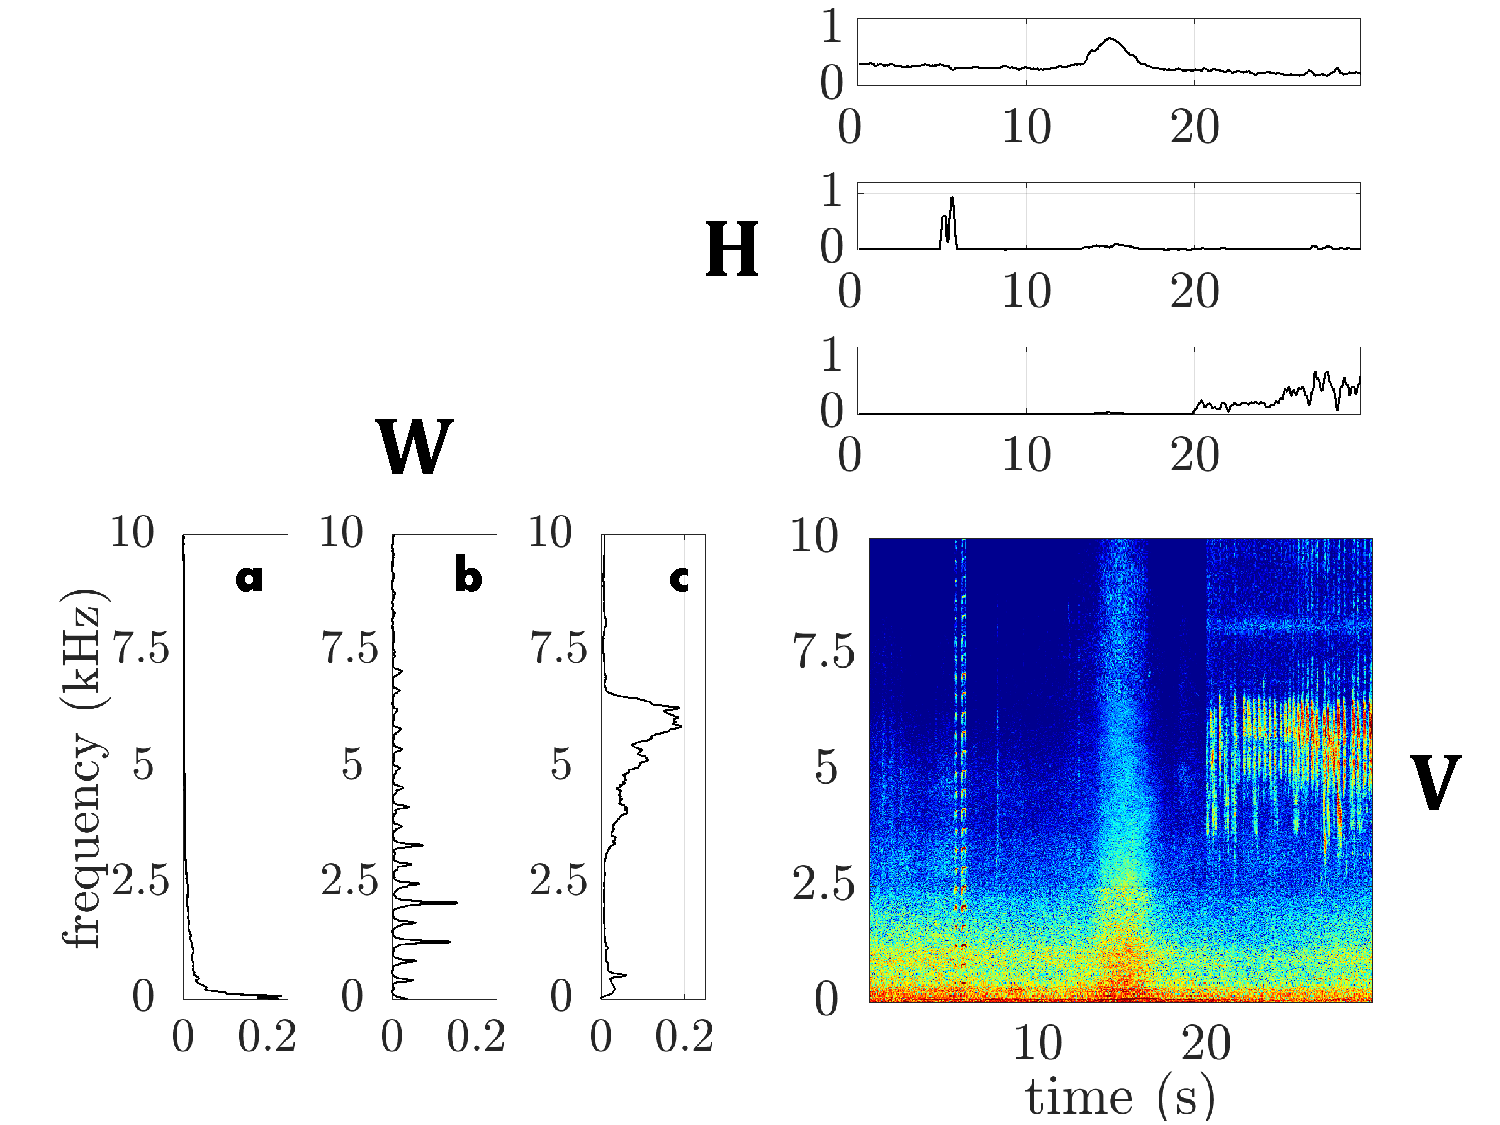
\includegraphics[width=0.9\linewidth]{figures/schema_introduction_nmf.pdf}
\caption{NMF decomposition of \DIFdelbeginFL \DIFdelFL{a }\DIFdelendFL \DIFaddbeginFL \DIFaddFL{an }\DIFaddendFL urban sound mixture comprising 3 sound events (car passages, car horn and bird's whistles), $\mathbf{W}$ is composed of 3 elements too ($K$ = 3) which correspond \DIFdelbeginFL \DIFdelFL{in }\DIFdelendFL \DIFaddbeginFL \DIFaddFL{to }\DIFaddendFL 3 audio spectra (car passages (a), car horn (b) and bird's whistles (c)).}
\label{fig:example_NMF}
\end{figure}
The choice of the dimensions is often made so that $F\times K + K \times N < F \times N$ \DIFaddbegin \DIFadd{\mbox{%DIFAUXCMD
\cite{fevotte_nonnegative_2009}}%DIFAUXCMD
}\DIFaddend . NMF is then considered as a low rank approximation method. However, this constraint is not mandatory. To estimate the quality of the approximation, an objective function is used

\begin{equation}\label{eq:min-D-WH}
\underset{\mathbf{H} \geq 0, \mathbf{W} \geq 0}{\min} D\left(\mathbf{V} \vert \vert \mathbf{\tilde{V}}\right).
\end{equation}

The operator $D(x\vert y)$ is a divergence calculation such as:
\begin{equation}
D\left(\textbf{V} \vert\vert \mathbf{\tilde{V}} \right) = \sum_{f = 1}^{F} \sum_{n = 1}^{N} d_{\beta}
\left(\textbf{V}_{fn} \vert \left[ \textbf{WH} \right]_{fn} \right)
\end{equation}

and usually belongs to the $\beta-$divergence class \cite{fevotte_nonnegative_2009} in which the well known Euclidean distance (eq. \ref{eq:def_distEUC}) and the Kullback-Leibler divergence (eq. \ref{eq:def_divKL}) belong

\begin{subequations}\label{eq:divBetaGenerale}
\begin{numcases}{d_{\beta}(x\vert y) =}
    \frac{1}{2}(x-y)^2, & $\beta = 2$, \label{eq:def_distEUC}\\
    x\log \dfrac{x}{y} - x + y, & $\beta = 1$.\label{eq:def_divKL}
\end{numcases}
\end{subequations}

To better take into account prior knowledge about the sources of interest, constraints (like the smoothness or the \DIFdelbegin \DIFdel{sparsness }\DIFdelend \DIFaddbegin \DIFadd{sparsity }\DIFaddend criteria \cite{virtanen_monaural_2007}) can be added to the objective function.

Algorithms have been proposed to solve the minimization problem (\ref{eq:min-D-WH}) iteratively such as the multiplicative update \cite{lee_algorithms_2000}, the alternating least square method \cite{cichocki_regularized_2007} or the projected gradient \cite{lin_projected_2007}. Here, the multiplicative update is chosen as it has been well studied in the literature and it ensures convergence of the results \cite{fevotte_algorithms_2011}.

\subsection{Supervised NMF}
First, supervised NMF (Sup-NMF) is used: the \textit{dictionary} includes audio spectra of urban sound sources. A lot of the different sound sources present in the urban environment are known. Their spectra can be obtained and be a basis of $\mathbf{W}$. The \textit{activation} matrix is then the unknown variable to estimate. In the first iteration, $\mathbf{H}$ is initialized randomly, then it is updated by the generic algorithm \cite{fevotte_algorithms_2011}

\begin{equation}\label{eq:updateH_Sup}
\textbf{H}^{(i+1)} \leftarrow \textbf{H}^{(i)}.\left(\frac{\textbf{W}^T \left[\left(\textbf{WH}^{(i)} \right)^{(\beta-2)}.\textbf{V} \right]}{\textbf{W}^T \left[\textbf{WH}^{(i)} \right]^{(\beta-1)}}\right)^{\gamma(\beta)}
\end{equation}

with $\gamma(\beta) = \frac{1}{2-\beta},$ for $\beta < 1$, $ \gamma(\beta) = 1$, for $\beta \in \left[1,2\right]$ and $\gamma(\beta) = \frac{1}{\beta-1}$ for $\beta > 2$. The product $A.B$ and $A/B$ are respectively the Hadamard product and ratio. As in the supervised approach the indexes of traffic components in $\mathbf{W}$  are known, the separation of the corresponding sound source is made by extracting the related basis and activators,

\begin{equation}\label{eq:separationExtraction}
\mathbf{\tilde{V}}_{traffic} = \left[ \mathbf{WH} \right]_{traffic}.
\end{equation}

\subsection{Semi-supervised NMF}

The supervised approach is useful when prior \DIFdelbegin \DIFdel{knowldge }\DIFdelend \DIFaddbegin \DIFadd{knowledge }\DIFaddend can be assumed for all the sources in the mixture, which is not a reasonable assumption in our application scenario. To some \DIFdelbegin \DIFdel{extend}\DIFdelend \DIFaddbegin \DIFadd{extent}\DIFaddend , prior knowledge can be considered for the traffic but not for the numerous kind of interferences that can occur in a realistic scenario. To better take into account the diverse nature of urban scenes, semi-supervised NMF (Sem-NMF)\cite{lee_semi-supervised_2010} is a good candidate as it offers more flexibility. This method assumes a \textit{dictionary} with a fixed part $\mathbf{W_s} \in \mathbb{R}^+_{F\times K}$, composed in our case of road traffic spectra, and with a mobile part, $\mathbf{W_r} \in \mathbb{R}^+_{F\times J}$ with $J <<K$, that is updated during optimization. In the literature, $J$ is set to a small number with respect to $K$ so as to force the optimization to still consider the fixed part of the dictionary \cite{lefevre2012semi}. The aim is to include in $\mathbf{W_r}$ the elements that are not related with the traffic. The problem (\ref{eq:nmf}) becomes

\begin{equation}
\mathbf{V} \approx \mathbf{\tilde{V}} = \mathbf{W_s H_s}+ \mathbf{W_r H_r}
\end{equation}

 with $\mathbf{W} = \left[\mathbf{W_s} \mathbf{W_r} \right]$ and $\mathbf{H} = \genfrac[]{0pt}{0}{\mathbf{H_s}}{\mathbf{H_r}}$. In a similar way as to solve the equation (\ref{eq:min-D-WH}), $\mathbf{W_r}$, $\mathbf{H_r}$ and $\mathbf{H_s}$ are successively updated with the relations (\ref{eq:WH-SSupdate}):

{\scriptsize
\begin{subequations}\label{eq:WH-SSupdate}
\begin{align}
\mathbf{W_r}^{(i+1)} &\leftarrow \mathbf{W_r}^{(i)}.\left(\frac{\left[\left(\mathbf{W_r H_r}^{(i)} \right)^{(\beta-2)}.\mathbf{V} \right]\mathbf{H_r}^T}{\left(\mathbf{W_r H_r}^{(i)} \right)^{(\beta-1)}\mathbf{H_r}^T}\right)^{\gamma(\beta)}, \label{eq:W_r_SS}\\
\mathbf{H_r}^{(i+1)} &\leftarrow \mathbf{H_r}^{(i)}.\left(\frac{\mathbf{W_r}^T \left[\left(\mathbf{W_r H_r}^{(i)} \right)^{(\beta-2)}.\mathbf{V} \right]}{\mathbf{W_r}^T \left(\mathbf{W_r H_r}^{(i)} \right)^{(\beta-1)}}\right)^{\gamma(\beta)}, \label{eq:H_r_SS}\\
\mathbf{H_s}^{(i+1)} &\leftarrow \mathbf{H_s}^{(i)}.\left(\frac{\mathbf{W_s}^T \left[\left(\mathbf{W_s H_s}^{(i)} \right)^{(\beta-2)}.\mathbf{V} \right]}{\mathbf{W_s}^T \left(\mathbf{W_s H_s}^{(i)} \right)^{(\beta-1)}}\right)^{\gamma(\beta)}.\label{eq:H_s_SS}
\end{align}
\end{subequations}}

Applications of Sem-NMF for speech denoising from background noise or musical content can be found in \cite{joder2012real} and \cite{weninger2012supervised}.

\subsection{Thresholded initialized NMF}

As it will be demonstrated in the experimental results described in Section \ref{part:results}, those last approaches fail to provide consistent results in a wide range of urban areas and for different traffic preponderances due to generalization capabilities issues.

We therefore propose an alternative scheme based on the unsupervised NMF. Usually in unsupervised \DIFaddbegin \DIFadd{learning}\DIFaddend , $\mathbf{W}$, as  $\mathbf{H}$, is initialized randomly. Here, as the concerned sound source is known and audio samples of car passages are available, an initial dictionary, $\mathbf{W_0}$, is learnt by converting the audio files in the spectra domain; see part \ref{part:dictionary_learning}. Then NMF is performed where $\mathbf{W}$ (eq. \ref{eq:updateW_unsup}) and $\mathbf{H}$ (eq.  \ref{eq:updateH_Sup}) are updated alternatively. $\mathbf{W}$ is therefore updated by forcing its \DIFdelbegin \DIFdel{initiation }\DIFdelend \DIFaddbegin \DIFadd{initialization }\DIFaddend with \textit{a priori} knowledge but allowing it to adapt to the actual content of the scene under study,

\begin{equation}\label{eq:updateW_unsup}
\textbf{W}^{(i+1)} \leftarrow \mathbf{W}^{(i)}.\left(\frac{\left[\left(\mathbf{W}^{(i)}\mathbf{H} \right)^{(\beta-2)}.\mathbf{V} \right]\mathbf{H}^T}{\left[\mathbf{W}^{(i)}\mathbf{H} \right]^{(\beta-1)}\mathbf{H}^T}\right)^{\gamma(\beta)}.
\end{equation}

After $N$ iterations, a measure of similarity $D_{\theta}\left(\mathbf{W_0} \vert \vert \mathbf{W} \right)$ between $\mathbf{W_0}$ and the obtained dictionary $\mathbf{W}$ for each element $k$ is computed using a cosine similarity metric,

\begin{equation}
D_{\theta}\left(\mathbf{W_0}_k \vert \vert \mathbf{W}_k \right) = \frac{\mathbf{W_0}_k.\mathbf{W}_k}{\vert \vert \mathbf{W_0}_k  \vert \vert . \vert \vert \mathbf{W}_k \vert \vert}.
\end{equation}

$D_{\theta}\left(\mathbf{W_0}_k \vert \vert \mathbf{W}_k \right) = 1$ means that the $k$-th element of $\mathbf{W}$ is identical to the $k$-th element of $\mathbf{W_0}$. \DIFdelbegin \DIFdel{In the opposite}\DIFdelend \DIFaddbegin \DIFadd{On the contrary}\DIFaddend , $D_{\theta}\left(\mathbf{W_0}_k \vert \vert \mathbf{W}_k \right)$ = 0 means that the elements are \DIFdelbegin \DIFdel{completely }\DIFdelend \DIFaddbegin \DIFadd{very }\DIFaddend different. This measure has the advantage to be bounded between 1 and 0 and to be invariant with respect to scale. The \DIFdelbegin \DIFdel{\mbox{%DIFAUXCMD
$k$
}%DIFAUXCMD
}\DIFdelend \DIFaddbegin \DIFadd{\mbox{%DIFAUXCMD
$K$
}%DIFAUXCMD
}\DIFaddend values of $D_{\theta}\left(\mathbf{W_0} \vert \vert \mathbf{W} \right)$ are next sorted in \DIFdelbegin \DIFdel{descending }\DIFdelend \DIFaddbegin \DIFadd{decreasing }\DIFaddend order. The elements in $\mathbf{W}$ that can belong to $\mathbf{W}_{traffic}$ are selected by a \textit{hard thresholding} method. It is defined as:

\begin{equation}
\mathbf{W}_k \in \mathbf{W}_{k,traffic} \quad \text{iff} \quad D\left(\mathbf{W_0}_k \vert \vert \mathbf{W}_{k} \right) > t
\end{equation}

where $t$ is a fixed threshold $\in [$ 0;1 $]$.
An illustrative example is displayed in Figure \ref{fig:W_TI_NMF}.\\

\begin{figure}
[t]
\centering
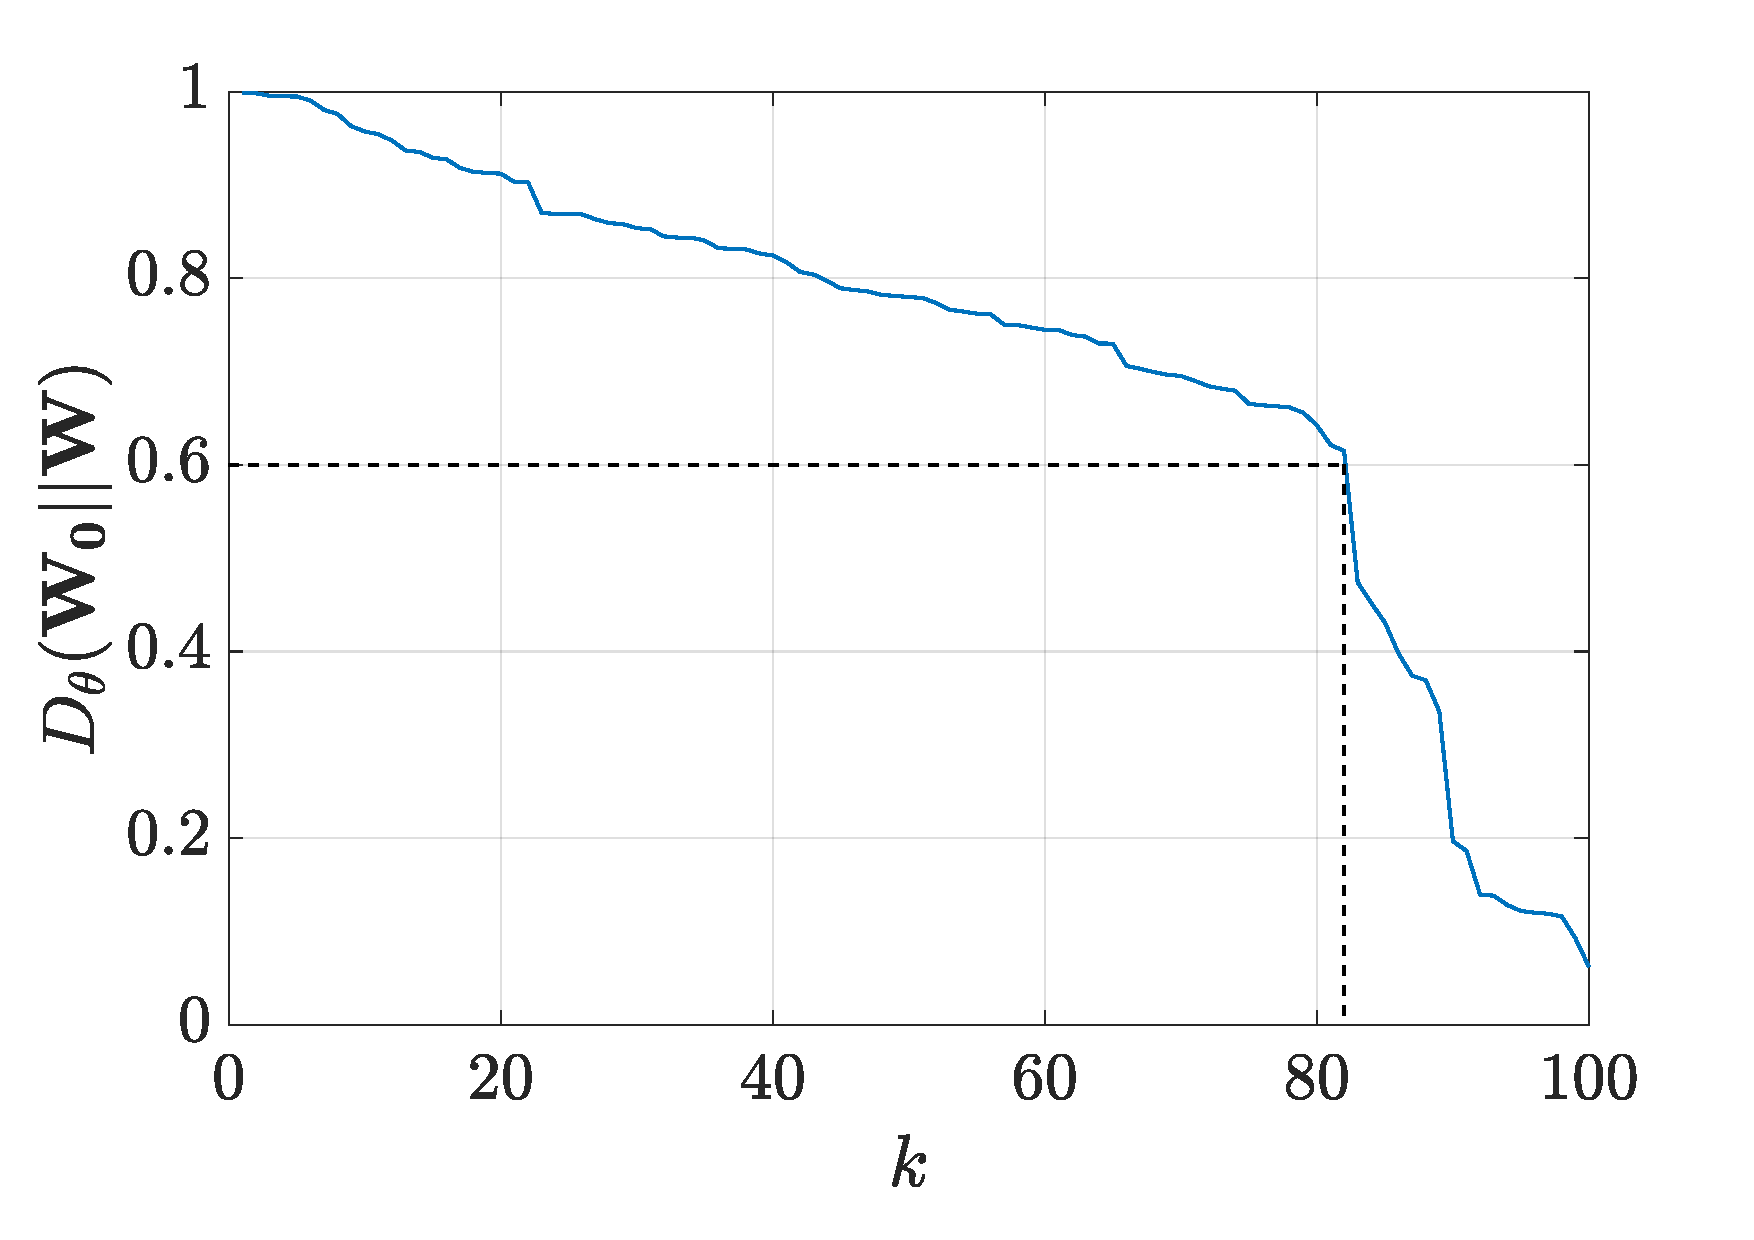
\includegraphics[width=0.8\linewidth]{figures/distanceCosLinDisplay.pdf}
\caption{$\mathbf{W}_{traffic}$ extraction from the sorted cosine similarity with a threshold $t = 0.6$. The \DIFdelbeginFL \DIFdelFL{\mbox{%DIFAUXCMD
$82$
}%DIFAUXCMD
-nd }\DIFdelendFL first \DIFaddbeginFL \DIFaddFL{\mbox{%DIFAUXCMD
$82$
}%DIFAUXCMD
}\DIFaddendFL elements are \DIFaddbeginFL \DIFaddFL{here }\DIFaddendFL considered as traffic component.}
\label{fig:W_TI_NMF}
\end{figure}
This approach is named \textit{Thresholded inititialized NMF} (TI-NMF). Other thresholding methods as the \textit{soft} \cite{donoho1995noising} and the \textit{firm} \cite{fornasier2008iterative} have been investigated. A \DIFdelbegin \DIFdel{fast }\DIFdelend \DIFaddbegin \DIFadd{quick }\DIFaddend parametric study revealed that the \textit{hard} thresholding method, as presented in  Figure \ref{fig:W_TI_NMF}, was the most \DIFaddbegin \DIFadd{simple and }\DIFaddend reliable approach.

\section{Experimental protocol}\label{part:protocol}

In order to validate the usefulness of the proposed NMF scheme to estimate the road traffic noise levels, one need to compare the traffic noise level predicted by the algorithm to a reference level. The latter can hardly be measured or even annotated from real life recordings. Thus,  we propose to consider simulated sound scenes to assess the performance of the proposed NMF. This offers a controlled framework to design at low cost a wide diversity of sound environments in which all the traffic components are known, thus allowing the computation of the reference level.

\subsection{Environmental sound scene corpus}

The corpus is designed with the \textit{SimScene} software\footnote{Open-source project available at: \url{https://bitbucket.org/mlagrange/simScene}}. \textit{SimScene} \cite{rossignol_simscene:_2015} is a simulator that creates monaural sound scenes \DIFdelbegin \DIFdel{in a .wav format }\DIFdelend by sequencing and summing audio samples that come from an isolated sound database. The simulator has been \DIFdelbegin \DIFdel{succesfully }\DIFdelend \DIFaddbegin \DIFadd{successfully }\DIFaddend considered for a wide range of experimental design for sound detection algorithm assessment \cite{lafay:hal-01111381} \cite{benetos:hal-01520194} \cite{mesaros:hal-01650601}.

This database is divided into two categories: $i)$ the \textit{event} category, which are the brief sounds (from 1 to 20 seconds) that are considered as salient including 245 sound event samples divided in 19 sound classes (\textit{ringing bell, whistling bird, sweeping broom, car horn, passing car, hammer, drill, coughing, barking dog, rolling suitcase, closing door, plane, siren, footstep, storm, street noise, metallic noise, train, tramway, truck and voice}) and $ii)$ the \textit{background} or \textit{texture} category that includes all the sounds that are of long duration and whose acoustic properties do not vary with respect to time. 154 sound samples that belong to this category are divided in 9 sound classes (\textit{whistling bird, construction site noise, crowd noise, park, rain, children playing in schoolyard, constant traffic noise, ventilation, wind}). These sounds are \DIFdelbegin \DIFdel{in .wav format }\DIFdelend sampled at 44.1 kHz. The sound class \textit{passing car} comes from 60 recordings of 2 cars (Renault Megane and Renault Scenic) made on the Ifsttar's runway at different speeds with multiple gear ratios. The other audio files have been found online (\textit{freesound.org}) and within the \textit{salamon2014dataset} database \cite{salamon_dataset_nodate}. Each sound class is composed of multiples samples (\textit{bird01.wav}, \textit{bird02.wav} \dots) to allow some diversity in the resulting mixture, see Figure \ref{fig:example_simScene}. The software allows the user to control some high level parameters (number of events of each class that appear in the mixture, elapsed time between each sample of a same class, presence of a fade in and a fade out \dots) completed with a standard deviation that may bring some \DIFdelbegin \DIFdel{random behavior }\DIFdelend \DIFaddbegin \DIFadd{compositional diversity }\DIFaddend between the scenes. Furthermore, an audio file of each sound class present in the scene can be generated that allows us to know its exact contribution as well as \DIFdelbegin \DIFdel{a text }\DIFdelend \DIFaddbegin \DIFadd{an annotation }\DIFaddend file that summarizes the time presence of all the events.\\


\begin{figure}
[t]
    \centering
       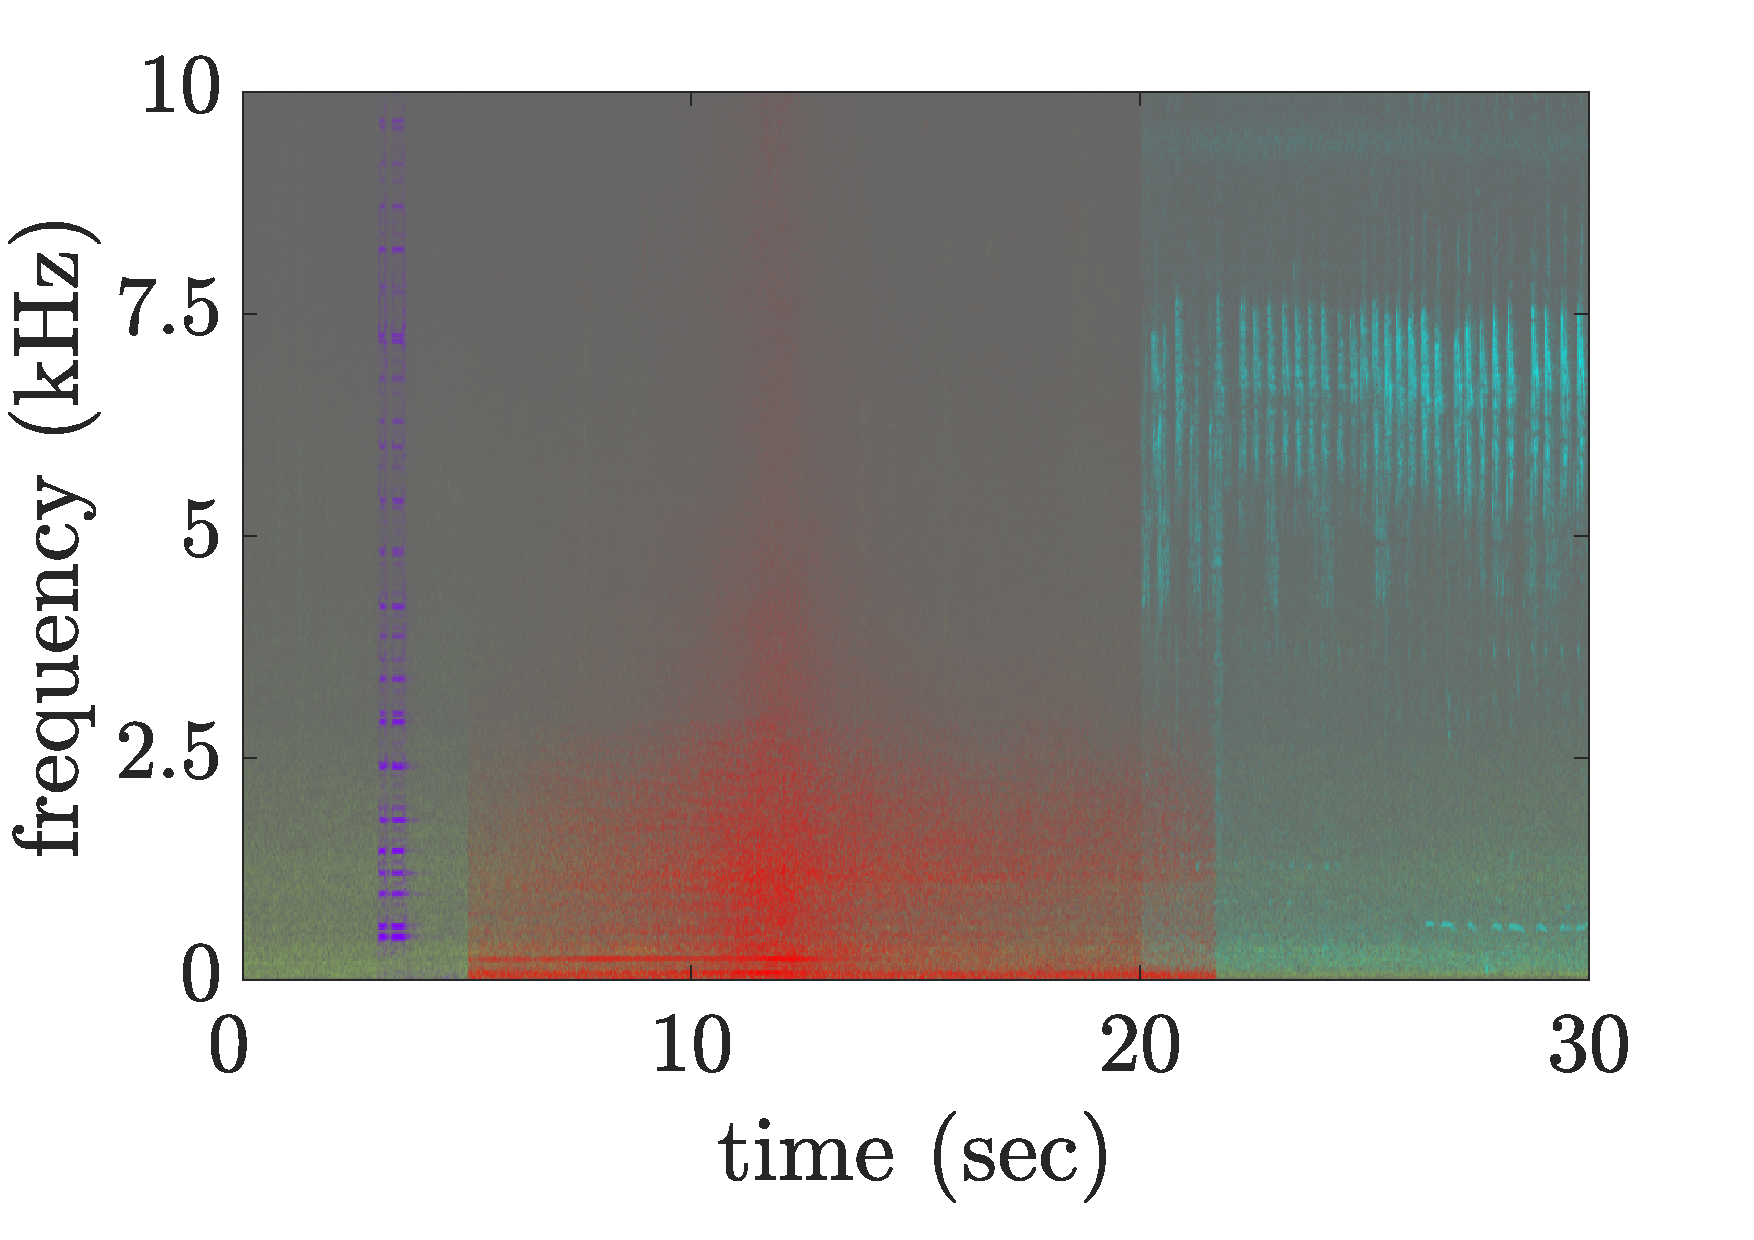
\includegraphics[width=.9\linewidth]{./figures/exampleSimScene}
    \caption{Spectrogram of a sound scene created with \textit{SimScene} software with a sound background (road traffic in green) and 3 sound events (car horn in purple, car passage in red and whistling bird in cyan).}
    \label{fig:example_simScene}
\end{figure}
This database allows the creation of a wide diversity of \DIFdelbegin \DIFdel{realistic }\DIFdelend urban sound scenes from the road traffic point of view \cite{gloaguen_creation_2017}. A sound mixing corpus is composed of 6 sub-corpus of 25 audio files each lasting 30 seconds. Each sub-corpus is characterized by a specific generic sound class that summed with traffic will make the estimation of the traffic level more difficult. The classes are: \textit{alert} (car horn, siren), \textit{animals} (barking dog , whistling bird), \textit{climate} (wind, rain), \textit{humans} (crowd noise and voice), \textit{mechanics} (metallic and construction site noises) and \textit{transportation} (train, tramway and plane). In each file, \DIFaddbegin \DIFadd{the }\DIFaddend traffic component is present\DIFdelbegin \DIFdel{as }\DIFdelend \DIFaddbegin \DIFadd{. What is called traffic component is }\DIFaddend the sum of the \DIFdelbegin \DIFdel{background and event traffic sounds while }\DIFdelend \DIFaddbegin \DIFadd{road traffic background noise and the sound events generated by the}\textit{\DIFadd{passing car}} \DIFadd{class. On the contrary, }\DIFaddend the \textit{interfering} sound class \DIFdelbegin \DIFdel{is the }\DIFdelend \DIFaddbegin \DIFadd{includes all the other }\DIFaddend sound sources not related to it. \DIFaddbegin \DIFadd{Car horn sound class belongs to the }\textit{\DIFadd{interfering}} \DIFadd{component as it is considered as a warning signal. }\DIFaddend To test different scenarios, each audio file is duplicated with the traffic sound level of the entire sound scene, $L_{p,traffic}$, fixed to a specific level according to the sound level of the interfering class, $L_{p,interfering}$,  following the relation (\ref{eq:tir}).

\begin{equation}\label{eq:tir}
TIR = L_{p,traffic}-L_{p,interfering}
\end{equation}

with \DIFaddbegin \DIFadd{\mbox{%DIFAUXCMD
$TIR$
}%DIFAUXCMD
, }\DIFaddend the \textit{Traffic Interference Ratio} \DIFdelbegin \DIFdel{\mbox{%DIFAUXCMD
$TIR \in$
}%DIFAUXCMD
\mbox{%DIFAUXCMD
$\lbrace$
}%DIFAUXCMD
12, -6, 0, 6, 12\mbox{%DIFAUXCMD
$\rbrace$
}%DIFAUXCMD
dB}\DIFdelend \DIFaddbegin \DIFadd{in a similar way to \mbox{%DIFAUXCMD
\cite{dikmen2013sound}}%DIFAUXCMD
}\DIFaddend . When $TIR < 0$ dB, the traffic component is less present than the interfering class. \DIFdelbegin \DIFdel{In the opposite}\DIFdelend \DIFaddbegin \DIFadd{On the contrary}\DIFaddend , for $TIR > 0$ dB, the traffic class is louder than the interfering class.
\DIFaddbegin \DIFadd{In most of the urban sound environments, the ratio between the interfering class and the traffic is mainly included between \mbox{%DIFAUXCMD
$TIR$
}%DIFAUXCMD
= -6 dB and \mbox{%DIFAUXCMD
$TIR$
}%DIFAUXCMD
= 12 dB \mbox{%DIFAUXCMD
\cite{gloaguen_creation_2017}}%DIFAUXCMD
. This is between these values that the estimator has to be the most efficient. But, in this experimental framework, this frame is extended to \mbox{%DIFAUXCMD
$TIR$
}%DIFAUXCMD
= -12 dB to test the limit of NMF. }\DIFaddend The total number of scenes designed is \DIFaddbegin \DIFadd{then }\DIFaddend 750 (6 sub-corpus $\times$ 25 scenes $\times$  5 $TIR$ values)\DIFaddbegin \DIFadd{, each scene during 30 seconds, it leads to a full duration of 6 hours and 30 minutes}\DIFaddend .

\subsection{Experiment}

The experiment consists in estimating the road traffic sound level of the 6 environmental sound sub-corpus (\textit{alert} (al\DIFaddbegin \DIFadd{.}\DIFaddend ), \textit{animals} (an\DIFaddbegin \DIFadd{.}\DIFaddend ), \textit{humans} (hu\DIFaddbegin \DIFadd{.}\DIFaddend ), \textit{climate} (cl\DIFdelbegin \DIFdel{), }\DIFdelend \DIFaddbegin \DIFadd{.), }\DIFaddend \textit{\DIFdelbegin \DIFdel{mechanics}\DIFdelend \DIFaddbegin \DIFadd{transportation}\DIFaddend } (\DIFdelbegin \DIFdel{me), }\DIFdelend \DIFaddbegin \DIFadd{tr.), }\DIFaddend \textit{\DIFdelbegin \DIFdel{transportation}\DIFdelend \DIFaddbegin \DIFadd{mechanics}\DIFaddend } (\DIFdelbegin \DIFdel{tr}\DIFdelend \DIFaddbegin \DIFadd{me.}\DIFaddend )) composed each of 25 audio files ($M$ = 25) and for 5 $TIR$ ($\lbrace$-12, -6, 0, 6, 12$\rbrace$ dB). The \DIFaddbegin \DIFadd{range of these values is large but in the urban environments, the \mbox{%DIFAUXCMD
$TIR$
}%DIFAUXCMD
seems to be between -6 dB and 12 dB \mbox{%DIFAUXCMD
\cite{gloaguen_creation_2017}}%DIFAUXCMD
. The case \mbox{%DIFAUXCMD
$TIR$
}%DIFAUXCMD
= -12 dB is then an extreme case to study the NMF behavior.
The }\DIFaddend spectrogram $\mathbf{V}$ of each sound scene is built with a window size $w = 2^{12}$ with a 50 $\%$ overlap, see Figure \ref{fig:bloc_experiment}.
\begin{figure}
    \centering
    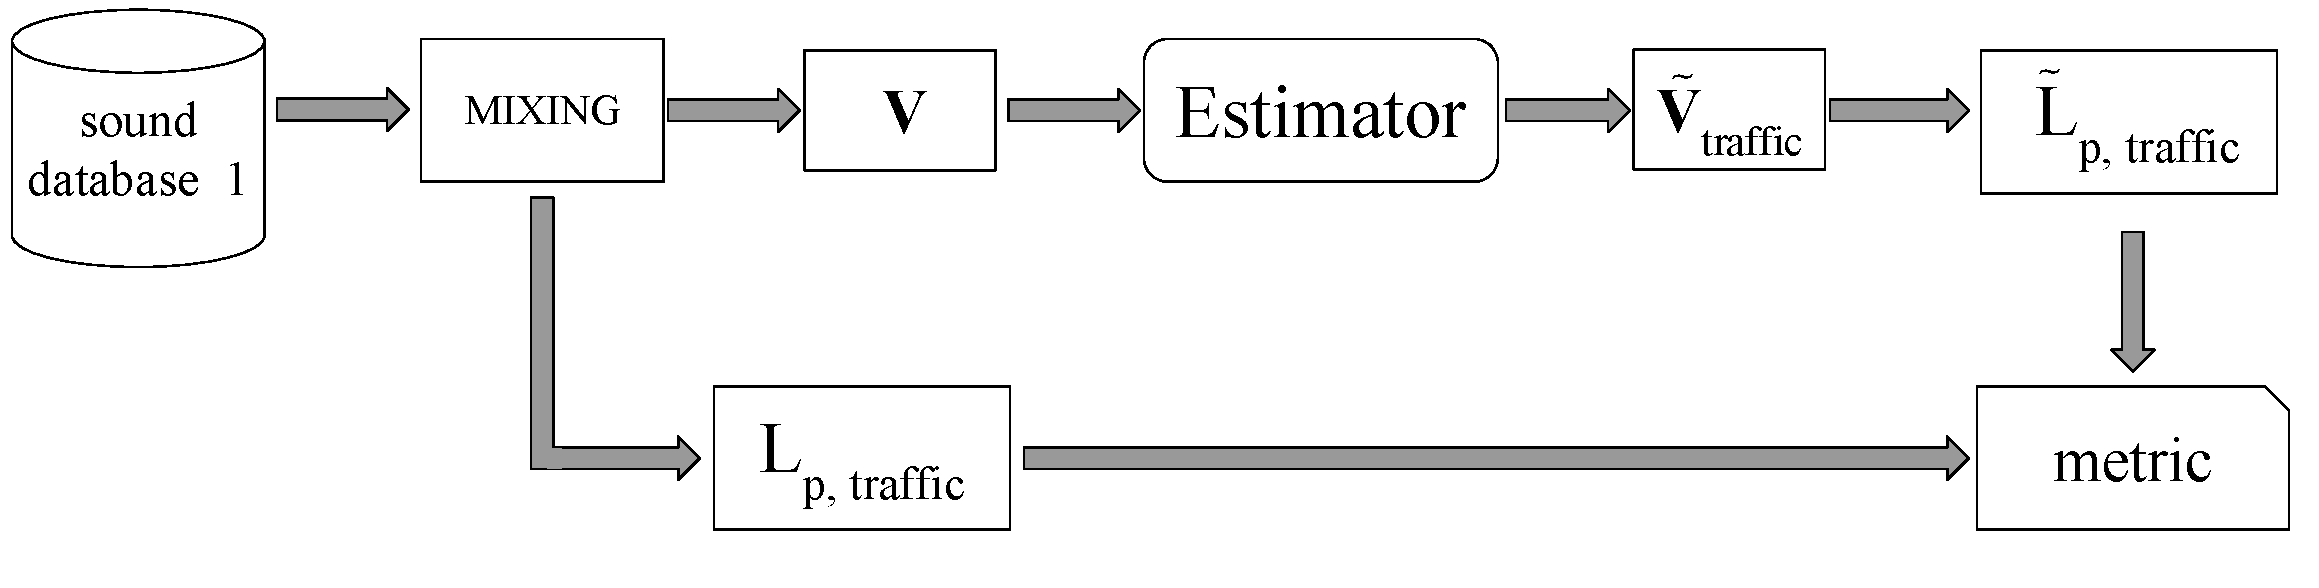
\includegraphics[width=\linewidth]{figures/bloc_diagram_estimator.pdf}
    \caption{Block diagram of the \DIFdelbeginFL \DIFdelFL{experience }\DIFdelendFL \DIFaddbeginFL \DIFaddFL{experiment }\DIFaddendFL with the urban sound scenes sound mixture step and the estimation step. The estimator may be a frequency low-pass filter or NMF.}
    \label{fig:bloc_experiment}
\end{figure}
Assuming that the traffic spectral profile is \DIFdelbegin \DIFdel{largely }\DIFdelend \DIFaddbegin \DIFadd{mostly }\DIFaddend concentrated in the low frequency components, a \DIFdelbegin \DIFdel{first }\DIFdelend \DIFaddbegin \DIFadd{simple }\DIFaddend estimator to determine the traffic sound level is a frequency low-pass filter. It \DIFdelbegin \DIFdel{depends only on the }\DIFdelend \DIFaddbegin \DIFadd{is parametrized only by its }\DIFaddend cut-off \DIFdelbegin \DIFdel{frequencies }\DIFdelend \DIFaddbegin \DIFadd{frequency }\DIFaddend $f_c \in  \lbrace$500, 1k, 2k, 5k, 10k, 20k$\rbrace$ Hz. The spectrogram $\mathbf{V}$ is filtered and the remaining energy is then considered as traffic component (eq. \ref{eq:v_tr_filtered}),

\begin{equation}\label{eq:v_tr_filtered}
\mathbf{\tilde{V}}_{traffic} = \mathbf{V}_{f_c}.
\end{equation}

The second estimator is the proposed scheme, based on \DIFaddbegin \DIFadd{one of }\DIFaddend the three NMF approaches presented in Section \ref{part:nmf}. Multiples experimental factors are involved here between the dictionary learning and NMF (see Figure \ref{fig:bloc_nmf}), each experimental factor having multiples modalities.
\begin{figure}
    \centering
    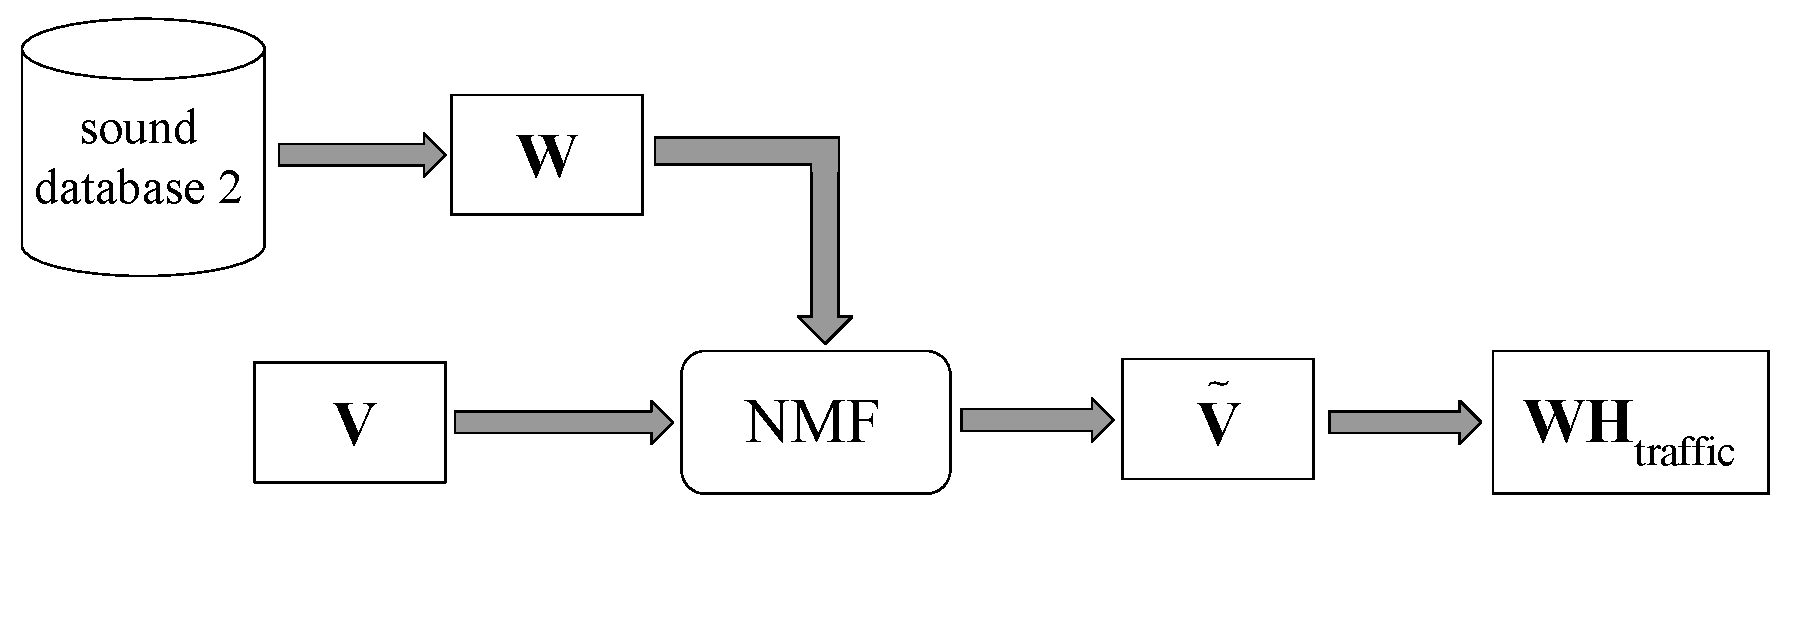
\includegraphics[width=\linewidth]{figures/bloc_diagram_NMF_EN_2.pdf}
    \caption{Specific block diagram of the NMF estimator with the dictionary design composed from a second sound database.}
    \label{fig:bloc_nmf}
\end{figure}
\begin{table*}[t]
\centering
\caption{Summary of the different experimental factors and their modalities taken into account in the \DIFdelbeginFL \DIFdelFL{frequency low-pass }\DIFdelendFL \DIFaddbeginFL \DIFaddFL{LP }\DIFaddendFL filter \DIFdelbeginFL \DIFdelFL{estimator}\DIFdelendFL \DIFaddbeginFL \DIFaddFL{and the NMF estimators}\DIFaddendFL .}
\DIFdelbeginFL %DIFDELCMD < \begin{tabularx}{17.5cm}{L{3cm}@{}C{12cm}@{}C{2cm}@{}}
%DIFDELCMD < 	%%%
\DIFdelendFL \DIFaddbeginFL \begin{tabularx}{17.5cm}{L{3cm}@{}C{12cm}@{}@{}C{2cm}}
	\DIFaddendFL \hline
    \textbf{\begin{tabular}[c]{@{}l@{}}experimental \\ factors\end{tabular}} & \textbf{modalities} &\begin{tabular}[c]{@{}C{2cm}@{}}\textbf{number}\\ \textbf{of modalities}\end{tabular}\\ \toprule
\end{tabularx}

\begin{tabularx}{17.5cm}{L{3cm}@{}C{2cm}@{}C{2cm}@{}@{}C{2cm}@{}@{}C{2cm}@{}@{}C{2cm}@{}@{}C{2cm}@{}@{}C{2cm}@{}}
    \textbf{sub-classes} & alert & animals & climate & humans & transportation & mechanics & 6
\end{tabularx}

\begin{tabularx}{17.5cm}{L{3cm}@{}C{2.4cm}@{}@{}C{2.4cm}@{}@{}C{2.4cm}@{}@{}C{2.4cm}@{}@{}C{2.4cm}@{}C{2cm}@{}}
\rowcolor[HTML]{C0C0C0}
   $\mathbf{TIR}$ (dB) & -12 & -6 & 0 & 6 & 12 & 5 \\
\end{tabularx}

\DIFdelbeginFL %DIFDELCMD < \begin{tabularx}{17.5cm}{L{3cm}@{}C{2cm}@{}C{2cm}@{}@{}C{2cm}@{}@{}C{2cm}@{}@{}C{2cm}@{}@{}C{2cm}@{}@{}C{2cm}@{}}
%DIFDELCMD <    %%%
\DIFdelFL{\mbox{%DIFAUXCMD
$\mathbf{f_c}$
}%DIFAUXCMD
(kHz) }%DIFDELCMD < & %%%
\DIFdelFL{0.5 }%DIFDELCMD < & %%%
\DIFdelFL{1 }%DIFDELCMD < & %%%
\DIFdelFL{2 }%DIFDELCMD < & %%%
\DIFdelFL{5 }\DIFdelendFL \DIFaddbeginFL \begin{tabularx}{17.5cm}{L{3cm}@{}C{3cm}@{}@{}C{3cm}@{}@{}C{3cm}@{}@{}C{3cm}@{}C{2cm}@{}}
  \textbf{\DIFaddFL{method}} \DIFaddendFL & \DIFdelbeginFL \DIFdelFL{10 }\DIFdelendFL \DIFaddbeginFL \DIFaddFL{LP filter }\DIFaddendFL & \DIFdelbeginFL \DIFdelFL{20  }\DIFdelendFL \DIFaddbeginFL \DIFaddFL{Sup-NMF }\DIFaddendFL & \DIFdelbeginFL \DIFdelFL{6}%DIFDELCMD < \\
%DIFDELCMD <    \bottomrule
%DIFDELCMD < \end{tabularx}
%DIFDELCMD < \label{tab:experimental_factorsFilter}
%DIFDELCMD < \end{table*}
%DIFDELCMD < 

%DIFDELCMD < \begin{table*}[t]
%DIFDELCMD < \centering
%DIFDELCMD < %%%
%DIFDELCMD < \caption{%
{%DIFAUXCMD
\DIFdelFL{Summary of the different experimental factors and their modalities taken into account in NMF estimator.}}
%DIFAUXCMD
%DIFDELCMD < \begin{tabularx}{17.5cm}{L{3cm}@{}C{12cm}@{}@{}C{2cm}}
%DIFDELCMD < 	\hline
%DIFDELCMD <     %%%
\textbf{%DIFDELCMD < \begin{tabular}[c]{@{}l@{}}%%%
\DIFdelFL{experimental }%DIFDELCMD < \\ %%%
\DIFdelFL{factors}%DIFDELCMD < \end{tabular}%%%
} %DIFAUXCMD
\DIFdelendFL \DIFaddbeginFL \DIFaddFL{Sem-NMF }\DIFaddendFL & \DIFdelbeginFL \textbf{\DIFdelFL{modalities}} %DIFAUXCMD
\DIFdelendFL \DIFaddbeginFL \DIFaddFL{TI-NMF }\DIFaddendFL & \DIFdelbeginFL %DIFDELCMD < \begin{tabular}[c]{@{}C{2cm}@{}}%%%
\textbf{\DIFdelFL{number}}%DIFAUXCMD
%DIFDELCMD < \\ %%%
\textbf{\DIFdelFL{of modalities}}%DIFAUXCMD
%DIFDELCMD < \end{tabular}%%%
\DIFdelendFL \DIFaddbeginFL \DIFaddFL{4 }\DIFaddendFL \\
\DIFdelbeginFL %DIFDELCMD < \toprule
%DIFDELCMD < %%%
\DIFdelendFL \end{tabularx}

\begin{tabularx}{17.5cm}{L{3cm}@{}C{2cm}@{}C{2cm}@{}@{}C{2cm}@{}@{}C{2cm}@{}@{}C{2cm}@{}@{}C{2cm}@{}@{}C{2cm}@{}}
\DIFdelbeginFL \textbf{\DIFdelFL{sub-classes}} %DIFAUXCMD
%DIFDELCMD < & %%%
\DIFdelFL{alert }%DIFDELCMD < & %%%
\DIFdelFL{animals }%DIFDELCMD < & %%%
\DIFdelFL{climate }%DIFDELCMD < & %%%
\DIFdelFL{humans }%DIFDELCMD < & %%%
\DIFdelFL{transportation }%DIFDELCMD < & %%%
\DIFdelFL{mechanics }%DIFDELCMD < & %%%
\DIFdelFL{6
}%DIFDELCMD < \end{tabularx}
%DIFDELCMD < 

%DIFDELCMD < \begin{tabularx}{17.5cm}{L{3cm}@{}C{2.4cm}@{}@{}C{2.4cm}@{}@{}C{2.4cm}@{}@{}C{2.4cm}@{}@{}C{2.4cm}@{}C{2cm}@{}}
%DIFDELCMD < %%%
\DIFdelendFL \rowcolor[HTML]{C0C0C0}
   \DIFdelbeginFL \DIFdelFL{\mbox{%DIFAUXCMD
$\mathbf{TIR}$
}%DIFAUXCMD
(dB}\DIFdelendFL \DIFaddbeginFL \DIFaddFL{\mbox{%DIFAUXCMD
$\mathbf{f_c}$
}%DIFAUXCMD
(kHz}\DIFaddendFL ) & \DIFdelbeginFL \DIFdelFL{-12 }%DIFDELCMD < & %%%
\DIFdelFL{-6 }%DIFDELCMD < & %%%
\DIFdelFL{0 }\DIFdelendFL \DIFaddbeginFL \DIFaddFL{0.5 }\DIFaddendFL & \DIFdelbeginFL \DIFdelFL{6 }\DIFdelendFL \DIFaddbeginFL \DIFaddFL{1 }\DIFaddendFL & \DIFdelbeginFL \DIFdelFL{12 }\DIFdelendFL \DIFaddbeginFL \DIFaddFL{2 }\DIFaddendFL & 5 \DIFdelbeginFL %DIFDELCMD < \\
%DIFDELCMD < \end{tabularx}
%DIFDELCMD < 

%DIFDELCMD < \begin{tabularx}{17.5cm}{L{3cm}@{}C{4cm}@{}@{}@{}C{4cm}@{}@{}C{4cm}@{}C{2cm}@{}}
%DIFDELCMD <   %%%
\textbf{\DIFdelFL{method}} %DIFAUXCMD
%DIFDELCMD < & %%%
\DIFdelFL{Sup-NMF }\DIFdelendFL & \DIFdelbeginFL \DIFdelFL{Sem-NMF }\DIFdelendFL \DIFaddbeginFL \DIFaddFL{10 }\DIFaddendFL & \DIFdelbeginFL \DIFdelFL{TI-NMF }\DIFdelendFL \DIFaddbeginFL \DIFaddFL{20  }\DIFaddendFL & \DIFdelbeginFL \DIFdelFL{3 }\DIFdelendFL \DIFaddbeginFL \DIFaddFL{6}\DIFaddendFL \\
\end{tabularx}

\begin{tabularx}{17.5cm}{L{3cm}@{}C{4cm}@{}@{}C{4cm}@{}@{}C{4cm}@{}C{2cm}@{}}
    \DIFdelbeginFL %DIFDELCMD < \rowcolor[HTML]{C0C0C0}
%DIFDELCMD <     %%%
\DIFdelendFL $\mathbf{w_t}$ (s) & 0.5 & 1 & \textit{all} & 3
\end{tabularx}

\begin{tabularx}{17.5cm}{L{3cm}@{}C{3cm}@{}@{}C{3cm}@{}@{}C{3cm}@{}@{}C{3cm}@{}C{2cm}@{}}
\DIFaddbeginFL \rowcolor[HTML]{C0C0C0}
    \DIFaddendFL $\mathbf{K}$ & 25 & 50 & 100 & 200  & 4\\
\end{tabularx}


\begin{tabularx}{17.5cm}{L{3cm}@{}C{6cm}@{}@{}C{6cm}@{}C{2cm}@{}}
   \DIFdelbeginFL %DIFDELCMD < \rowcolor[HTML]{C0C0C0}
%DIFDELCMD <    %%%
\DIFdelendFL $\mathbf{\beta}$ & 1 & 2 & 2\\
\end{tabularx}

\begin{tabularx}{17.5cm}{L{3cm}@{}C{12cm}@{}C{2cm}@{}}
\DIFaddbeginFL \rowcolor[HTML]{C0C0C0}
   \DIFaddendFL threshold $\mathbf{t}$  &  from 0.30 to 0.70 with 0.01 step & 41\\
   \bottomrule
\end{tabularx}

\label{tab:experimental_factorsNMF}
\end{table*}


\subsubsection{NMF Dictionary}\label{part:dictionary_learning}

In order to prevent potential overfitting issues, the dictionary is built from a separate sound database dedicated specifically to this task. \DIFdelbegin \DIFdel{It }\DIFdelend \DIFaddbegin \DIFadd{The train database }\DIFaddend is composed of 53 audio files of \DIFdelbegin \DIFdel{passing cars}\DIFdelend \DIFaddbegin \DIFadd{isolated passing cars with a 18 minutes and 29 seconds cumulative duration}\DIFaddend . These recordings have been made on the Ifsttar's runway too, with the same experimental conditions that the recordings of the \textit{SimScene} database but with two different cars (Dacia Sandero and Renault Clio). \DIFaddbegin \DIFadd{The different steps leading to a dictionary is resumed in Figure \ref{fig:creation_W}. }\DIFaddend First, for each audio file, its spectrogram is calculated with fixed parameters ($w$, 50 $\%$ overlap, $nfft$). Then time/frequency windows of $F \times w_t $ dimensions are applied without overlapping on the spectrogram in order to consider several spectra for each audio file where $w_t \in \lbrace$0.5, 1$\rbrace$ second. In each window, the root mean square value is calculated on each frequency bin to reduce the windowed spectrogram in one spectrum a of $F \times 1$ dimension. With this size of window, it is possible to obtain the characteristic pitches of the different audio samples. One obtains for each value of $w_t$, from the 53 audio samples of passing cars respectively 2218 and 1109 elements. Since the number of elements given by this processing is high, in order to reduce the computational time and avoid redundant information, a $K$-means clustering algorithm is applied to reduce the number of spectra to $K \in \lbrace$25, 50, 100, 200$\rbrace$. The $K$ centroids are then the elements considered in the dictionary. A special case is added where the root mean square of \textit{all} the spectrogram is applied ($w_t$ = $all$) to build a dictionary with the spectral envelope of each audio sample. In this case, 53 spectra are obtained. The $K$-means clustering algorithm is then reduced to $K \in \lbrace$25, 50$\rbrace$.

\begin{figure}
[t]
\centering
\DIFaddbeginFL 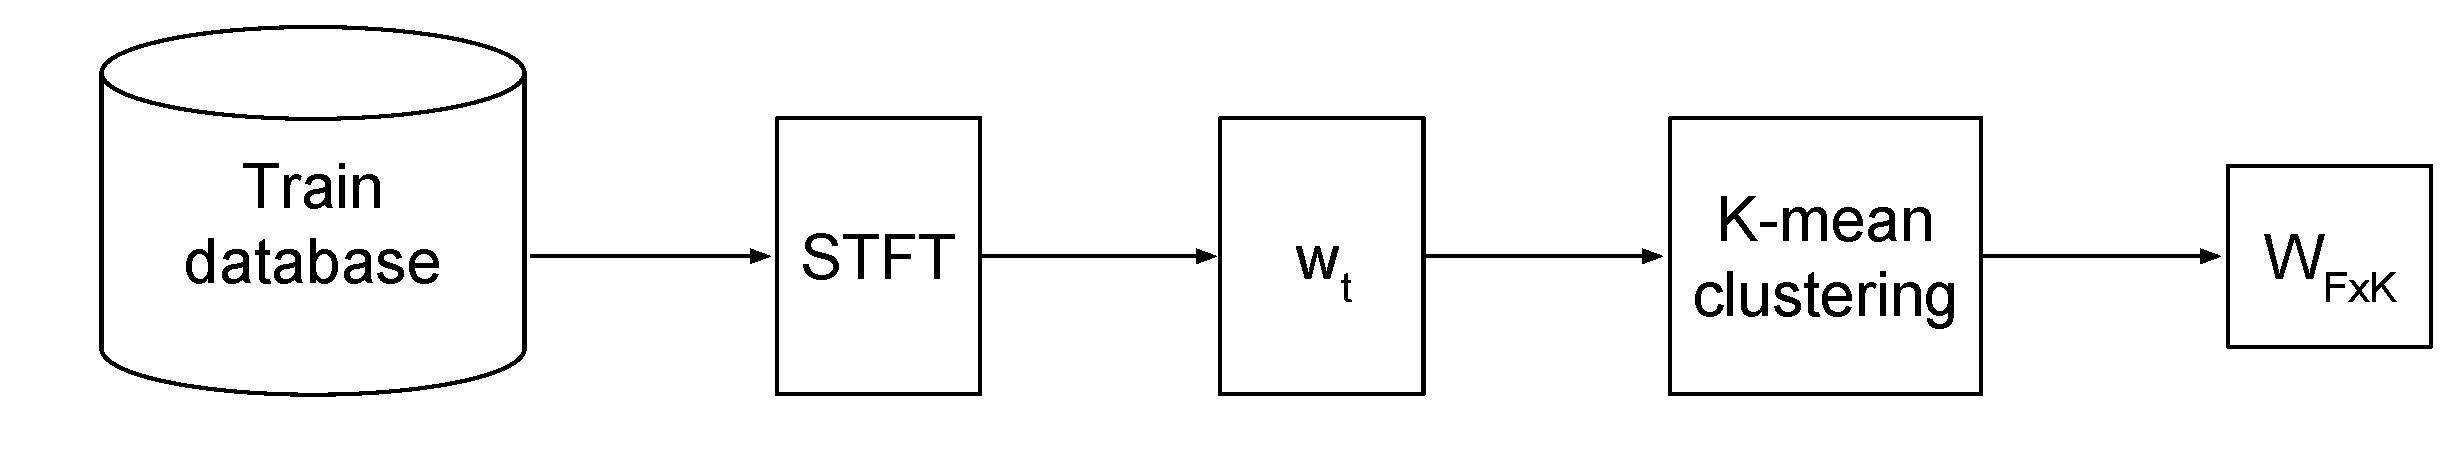
\includegraphics[width=\linewidth]{figures/creation_W_EN.pdf}
\caption{\DIFaddFL{Steps involved in the dictionary learning.}}
\label{fig:creation_W}
\end{figure}
\begin{figure}
[t]
  \centering
  \DIFaddendFL \subfloat[]{\label{fig:specW}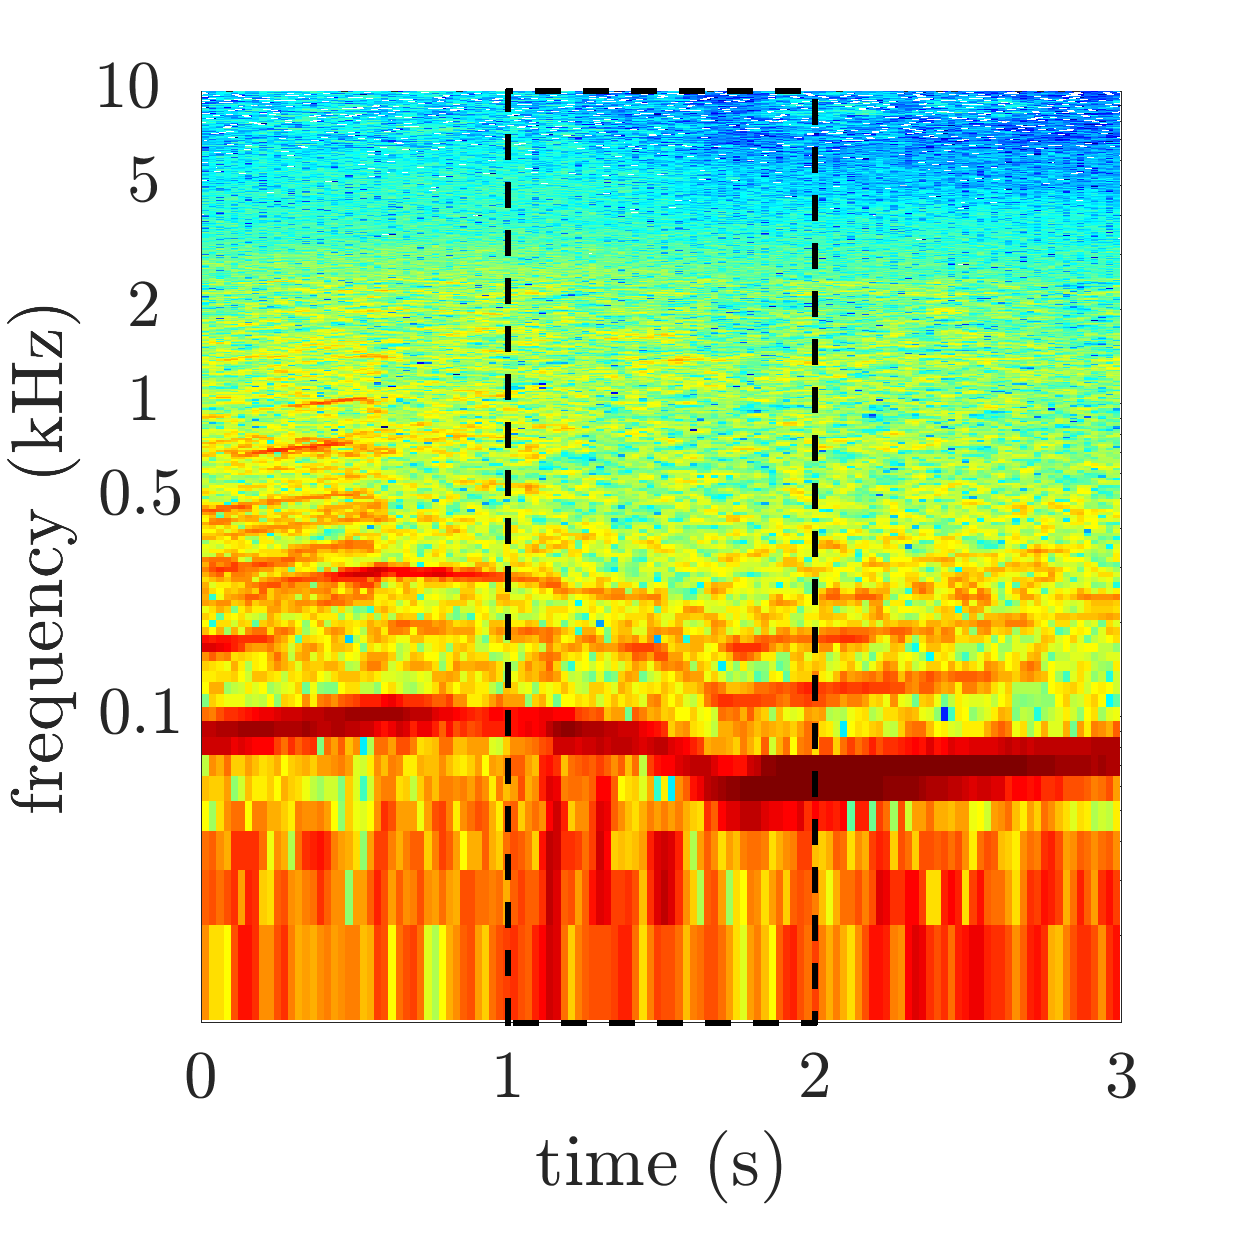
\includegraphics[width=.45\linewidth]{figures/dictionary3.pdf}}
%  \hspace{5pt}
  \subfloat[]{\label{fig:ElementW}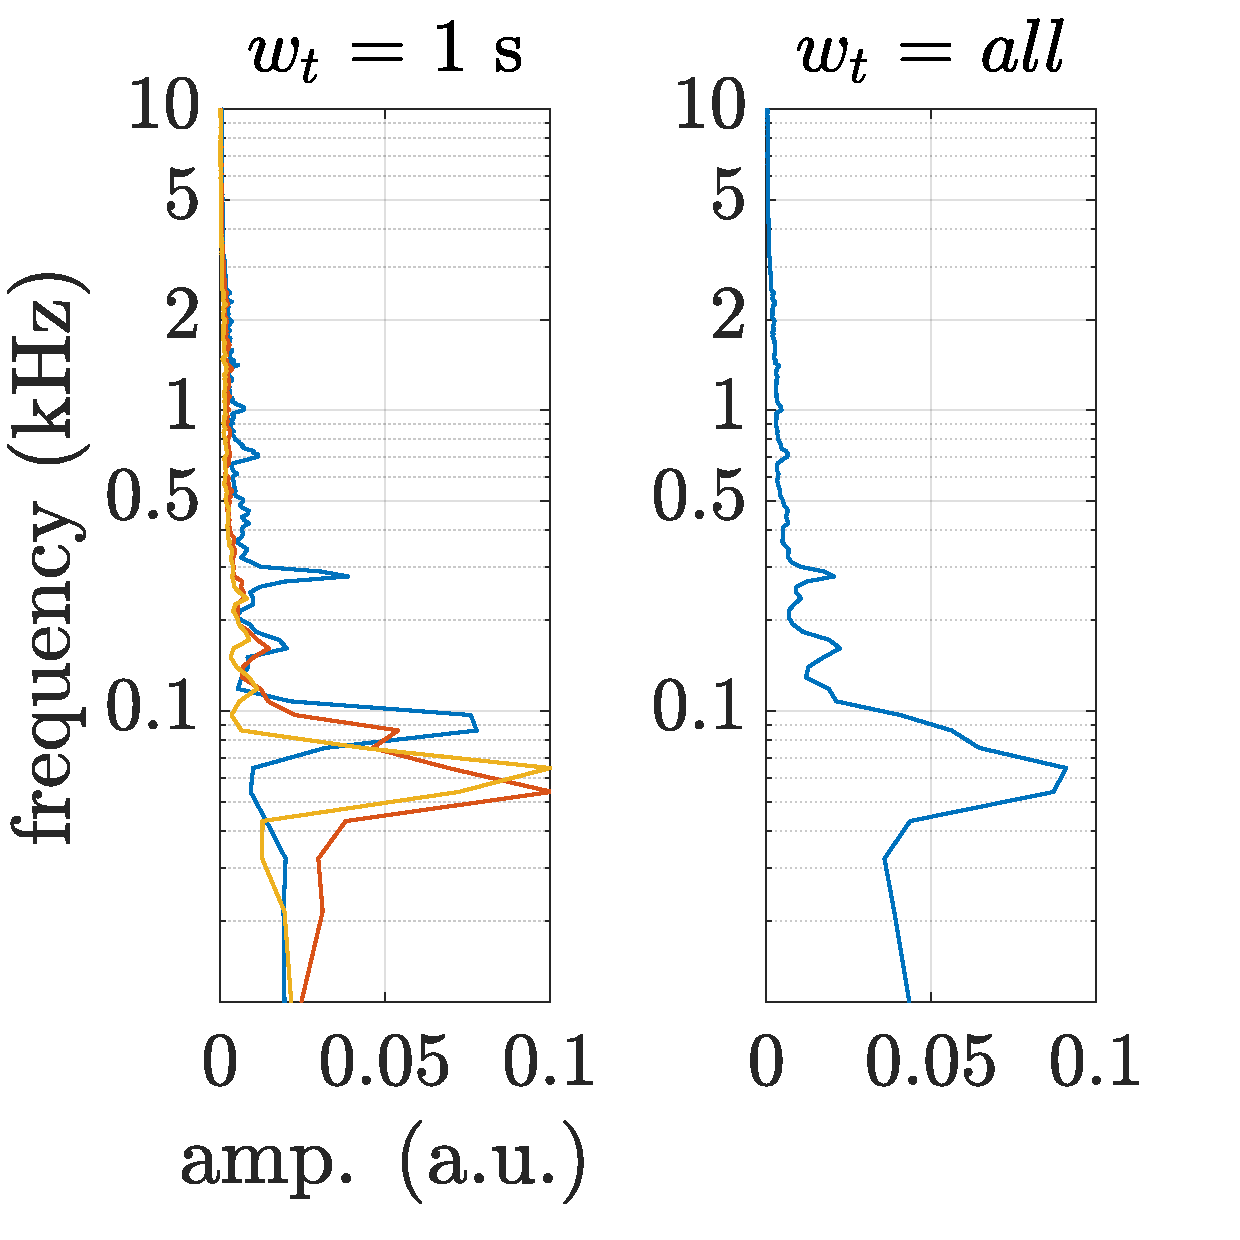
\includegraphics[width=.45\linewidth]{figures/dictionary4.pdf}}
  \caption{Dictionary building on a 3 second extract of a car passage. In dashed lines, a 1 second $w_t$ window  (\ref{fig:specW}). With $w_t$ = 1 second, 3 spectra are then generated and included in $\mathbf{W}$, while for $w_t$ = $all$, the audio file is reduced into 1 spectral vector (\ref{fig:ElementW}).}
  \label{fig:spec_elementW}
\end{figure}
An example that illustrates the process can be found on Figure \ref{fig:spec_elementW} on a 3 second extract of the spectrogram of a car passage, see Figure \ref{fig:specW}. In the case where $w_t$ = 1 second, 3 elements are therefore extracted from the spectrogram while in the case where $w_t$ = \textit{all}, all the spectrogram is reduced into one element, see Figure \ref{fig:ElementW}.

\DIFdelbegin \DIFdel{The obtained dictionary is expressed with third octave bands and each }\DIFdelend \DIFaddbegin \DIFadd{Each }\DIFaddend basis vector of $\mathbf{W}$ is normalized such as $\vert \vert \mathbf{W_k} \vert \vert = 1$ with $\vert \vert \bullet \vert\vert$ the $\ell$-1 norm. Table \ref{tab:experimental_factorsNMF} summarizes the experimental factors ($K$ and $w_t$) for the dictionary building and their related modalities. \DIFdelbegin \DIFdel{This last step allows us to reduce the dimensionality while preserving a rich description of the spectral content. Experimental validation consistently showed that considering octave bands do not impact the performance of the estimator studied in this paper}\DIFdelend \DIFaddbegin \DIFadd{The 10 versions of the built dictionary are then used for NMF. In Sup-NMF, these 10 versions correspond to \mbox{%DIFAUXCMD
$\mathbf{W}$
}%DIFAUXCMD
, in Sem-NMF, they correspond to the fixed part \mbox{%DIFAUXCMD
$\mathbf{W_s}$
}%DIFAUXCMD
and for TI-NMF, they are the initial dictionaries \mbox{%DIFAUXCMD
$\mathbf{W_0}$
}%DIFAUXCMD
that are next updated}\DIFaddend .

\begin{table*}[t]
\centering
\caption{Best results for all the scenes according to the experimental factors $\beta$ and \textit{method} (in bold letter, the lowest error).}
\begin{tabular}{@{}ccccccc@{}}
\toprule
\textbf{method} & $f_c$ (kHz) & $\mathbf{\beta}$ & $\mathbf{K}$ & $\mathbf{w_t}$ (s) &   $\mathbf{t}$ & \textbf{$MAE$} (dB) \\ \midrule
filter & 20  & \DIFaddbeginFL \DIFaddFL{- }\DIFaddendFL & \DIFaddbeginFL \DIFaddFL{- }\DIFaddendFL & \DIFaddbeginFL \DIFaddFL{- }\DIFaddendFL & \DIFaddbeginFL \DIFaddFL{- }\DIFaddendFL & 4.69 ($\pm$ 4.52) \\
filter & 0.5 & \DIFaddbeginFL \DIFaddFL{- }\DIFaddendFL &\DIFaddbeginFL \DIFaddFL{-  }\DIFaddendFL & \DIFaddbeginFL \DIFaddFL{- }\DIFaddendFL & \DIFaddbeginFL \DIFaddFL{- }\DIFaddendFL & 2.89 ($\pm$ 2.84) \\ \hline \hline
Sup-NMF & \DIFaddbeginFL \DIFaddFL{- }\DIFaddendFL & 1 & \DIFdelbeginFL \DIFdelFL{50 }\DIFdelendFL \DIFaddbeginFL \DIFaddFL{25 }\DIFaddendFL & \DIFdelbeginFL \DIFdelFL{0.5  }\DIFdelendFL \DIFaddbeginFL \DIFaddFL{\mbox{%DIFAUXCMD
$all$
}%DIFAUXCMD
}\DIFaddendFL & \DIFaddbeginFL \DIFaddFL{- }\DIFaddendFL & \DIFdelbeginFL \DIFdelFL{3.44 }\DIFdelendFL \DIFaddbeginFL \DIFaddFL{3.45 }\DIFaddendFL ($\pm$ 3.70) \\
Sup-NMF & \DIFaddbeginFL \DIFaddFL{- }\DIFaddendFL & 2 & \DIFdelbeginFL \DIFdelFL{50 }\DIFdelendFL \DIFaddbeginFL \DIFaddFL{25 }\DIFaddendFL & \DIFdelbeginFL \DIFdelFL{0.5  }\DIFdelendFL \DIFaddbeginFL \DIFaddFL{2  }\DIFaddendFL & \DIFaddbeginFL \DIFaddFL{- }\DIFaddendFL & \DIFdelbeginFL \DIFdelFL{3.02 }\DIFdelendFL \DIFaddbeginFL \DIFaddFL{2.84 }\DIFaddendFL ($\pm$ \DIFdelbeginFL \DIFdelFL{3.33}\DIFdelendFL \DIFaddbeginFL \DIFaddFL{3.19}\DIFaddendFL ) \\ \hline \hline
Sem-NMF & \DIFaddbeginFL \DIFaddFL{- }\DIFaddendFL & 1 & \DIFdelbeginFL \DIFdelFL{100 }\DIFdelendFL \DIFaddbeginFL \DIFaddFL{200 }\DIFaddendFL & \DIFdelbeginFL \DIFdelFL{0.5 }\DIFdelendFL \DIFaddbeginFL \DIFaddFL{2 }\DIFaddendFL & \DIFaddbeginFL \DIFaddFL{-  }\DIFaddendFL & \DIFdelbeginFL \DIFdelFL{2.33 }\DIFdelendFL \DIFaddbeginFL \DIFaddFL{2.32 }\DIFaddendFL ($\pm$ \DIFdelbeginFL \DIFdelFL{1.10}\DIFdelendFL \DIFaddbeginFL \DIFaddFL{1.15}\DIFaddendFL ) \\
Sem-NMF & \DIFaddbeginFL \DIFaddFL{- }\DIFaddendFL & 2 & \DIFdelbeginFL \DIFdelFL{100 }\DIFdelendFL \DIFaddbeginFL \DIFaddFL{200 }\DIFaddendFL & \DIFdelbeginFL \DIFdelFL{0.5 }\DIFdelendFL \DIFaddbeginFL \DIFaddFL{2 }\DIFaddendFL & \DIFaddbeginFL \DIFaddFL{-  }\DIFaddendFL & 2.32 ($\pm$ 1.26) \\ \hline \hline
\textbf{TI-NMF} & \DIFaddbeginFL \DIFaddFL{- }\DIFaddendFL & \textbf{1} & \textbf{200} & \textbf{0.5} &  \textbf{\DIFdelbeginFL \DIFdelFL{0.42}\DIFdelendFL \DIFaddbeginFL \DIFaddFL{0.41}\DIFaddendFL } &\textbf{\DIFdelbeginFL \DIFdelFL{2.19 }\DIFdelendFL \DIFaddbeginFL \DIFaddFL{2.15 }\DIFaddendFL ($\pm$ \DIFdelbeginFL \DIFdelFL{2.18}\DIFdelendFL \DIFaddbeginFL \DIFaddFL{2.10}\DIFaddendFL )} \\
TI-NMF & \DIFaddbeginFL \DIFaddFL{- }\DIFaddendFL & 2 & \DIFdelbeginFL \DIFdelFL{25 }%DIFDELCMD < & %%%
\DIFdelFL{all }%DIFDELCMD < &  %%%
\DIFdelFL{0.54 }%DIFDELCMD < & %%%
\DIFdelFL{2.20 (\mbox{%DIFAUXCMD
$\pm$
}%DIFAUXCMD
2.26)}%DIFDELCMD < \\ \bottomrule
%DIFDELCMD < \end{tabular}
%DIFDELCMD < %DIFDELCMD < \label{tab:results}%%%
%DIFDELCMD < \end{table*}
%DIFDELCMD < 

%DIFDELCMD < \begin{table*}[t]
%DIFDELCMD < \centering
%DIFDELCMD < %%%
%DIFDELCMD < \caption{%
{%DIFAUXCMD
\DIFdelFL{\mbox{%DIFAUXCMD
$MAE$
}%DIFAUXCMD
error averaged on all sub-classes on each \mbox{%DIFAUXCMD
$TIR$
}%DIFAUXCMD
for the best scenario according to each method.}}
%DIFAUXCMD
%DIFDELCMD < \begin{tabular}{@{}cccccc@{}}
%DIFDELCMD < \toprule
%DIFDELCMD < %%%
\textbf{\DIFdelFL{method}} %DIFAUXCMD
%DIFDELCMD < & %%%
\DIFdelFL{filter }%DIFDELCMD < & %%%
\DIFdelFL{filter }%DIFDELCMD < & %%%
\DIFdelFL{Sup-NMF }%DIFDELCMD < & %%%
\DIFdelFL{Sem-NMF }%DIFDELCMD < & %%%
\DIFdelFL{TI-NMF }%DIFDELCMD < \\ \midrule
%DIFDELCMD < %%%
\DIFdelFL{\mbox{%DIFAUXCMD
$f_c$
}%DIFAUXCMD
(kHz) }%DIFDELCMD < & %%%
\DIFdelFL{20 }\DIFdelendFL \DIFaddbeginFL \DIFaddFL{200 }\DIFaddendFL & 0.5 &  \DIFaddbeginFL \DIFaddFL{0.36 }\DIFaddendFL & \DIFdelbeginFL %DIFDELCMD < &  \\
%DIFDELCMD < %%%
\DIFdelFL{\mbox{%DIFAUXCMD
$\mathbf{\beta}$
}%DIFAUXCMD
}%DIFDELCMD < &  &  & %%%
\DIFdelFL{2 }%DIFDELCMD < & %%%
\DIFdelFL{2 }%DIFDELCMD < & %%%
\DIFdelFL{1 }%DIFDELCMD < \\ \hline
%DIFDELCMD < %%%
\textbf{\DIFdelFL{-12}} %DIFAUXCMD
%DIFDELCMD < & %%%
\DIFdelFL{12.25 (\mbox{%DIFAUXCMD
$\pm$
}%DIFAUXCMD
0.05) }%DIFDELCMD < & %%%
\DIFdelFL{7.36 (\mbox{%DIFAUXCMD
$\pm$
}%DIFAUXCMD
3.00) }%DIFDELCMD < & %%%
\DIFdelFL{8.65 (\mbox{%DIFAUXCMD
$\pm$
}%DIFAUXCMD
1.88) }%DIFDELCMD < & %%%
\DIFdelFL{3.88 (\mbox{%DIFAUXCMD
$\pm$
}%DIFAUXCMD
1.52) }%DIFDELCMD < & %%%
\DIFdelFL{5.35 (\mbox{%DIFAUXCMD
$\pm$
}%DIFAUXCMD
2.71) }%DIFDELCMD < \\
%DIFDELCMD < %%%
\textbf{\DIFdelFL{-6}} %DIFAUXCMD
%DIFDELCMD < & %%%
\DIFdelFL{6.96 (\mbox{%DIFAUXCMD
$\pm$
}%DIFAUXCMD
0.05) }%DIFDELCMD < & %%%
\DIFdelFL{3.44 (\mbox{%DIFAUXCMD
$\pm$
}%DIFAUXCMD
1.65) }%DIFDELCMD < & %%%
\DIFdelFL{4.22 (\mbox{%DIFAUXCMD
$\pm$
}%DIFAUXCMD
1.27) }%DIFDELCMD < & %%%
\DIFdelFL{1.37 (\mbox{%DIFAUXCMD
$\pm$
}%DIFAUXCMD
0.71)  }%DIFDELCMD < & %%%
\DIFdelFL{2.82 (\mbox{%DIFAUXCMD
$\pm$
}%DIFAUXCMD
1.30) }%DIFDELCMD < \\
%DIFDELCMD < %%%
\textbf{\DIFdelFL{0}} %DIFAUXCMD
%DIFDELCMD < & %%%
\DIFdelFL{3.00 (\mbox{%DIFAUXCMD
$\pm$
}%DIFAUXCMD
0.03) }%DIFDELCMD < & %%%
\DIFdelFL{1.17 (\mbox{%DIFAUXCMD
$\pm$
}%DIFAUXCMD
0.24) }%DIFDELCMD < & %%%
\DIFdelFL{1.34 (\mbox{%DIFAUXCMD
$\pm$
}%DIFAUXCMD
0.56) }%DIFDELCMD < & %%%
\DIFdelFL{1.11 (\mbox{%DIFAUXCMD
$\pm$
}%DIFAUXCMD
0.25) }%DIFDELCMD < & %%%
\DIFdelFL{1.26 (\mbox{%DIFAUXCMD
$\pm$
}%DIFAUXCMD
0.35) }%DIFDELCMD < \\
%DIFDELCMD < %%%
\textbf{\DIFdelFL{6}} %DIFAUXCMD
%DIFDELCMD < & %%%
\DIFdelFL{0.25 (\mbox{%DIFAUXCMD
$\pm$
}%DIFAUXCMD
0.06) }%DIFDELCMD < & %%%
\DIFdelFL{1.03 (\mbox{%DIFAUXCMD
$\pm$
}%DIFAUXCMD
0.26) }%DIFDELCMD < & %%%
\DIFdelFL{0.26 (\mbox{%DIFAUXCMD
$\pm$
}%DIFAUXCMD
0.10) }%DIFDELCMD < & %%%
\DIFdelFL{2.25 (\mbox{%DIFAUXCMD
$\pm$
}%DIFAUXCMD
0.19) }%DIFDELCMD < & %%%
\DIFdelFL{0.70 (\mbox{%DIFAUXCMD
$\pm$
}%DIFAUXCMD
0.32) }%DIFDELCMD < \\
%DIFDELCMD < %%%
\textbf{\DIFdelFL{12}} %DIFAUXCMD
%DIFDELCMD < & %%%
\DIFdelFL{0.26 (\mbox{%DIFAUXCMD
$\pm$
}%DIFAUXCMD
0.00) }%DIFDELCMD < & %%%
\DIFdelFL{1.45 (\mbox{%DIFAUXCMD
$\pm$
}%DIFAUXCMD
0.13) }%DIFDELCMD < & %%%
\DIFdelFL{0.64 (\mbox{%DIFAUXCMD
$\pm$
}%DIFAUXCMD
0.06) }%DIFDELCMD < & %%%
\DIFdelFL{2.96 (\mbox{%DIFAUXCMD
$\pm$
}%DIFAUXCMD
0.21)  }%DIFDELCMD < & %%%
\DIFdelFL{0.84 }\DIFdelendFL \DIFaddbeginFL \DIFaddFL{2.29 }\DIFaddendFL ($\pm$ \DIFdelbeginFL \DIFdelFL{0.24}\DIFdelendFL \DIFaddbeginFL \DIFaddFL{2.40}\DIFaddendFL )\\ \bottomrule
\end{tabular}
\DIFdelbeginFL %DIFDELCMD < \label{tab:results_TIR}
%DIFDELCMD < %%%
\DIFdelendFL \DIFaddbeginFL \label{tab:results}
\DIFaddendFL \end{table*}


\subsubsection{Experimental factors of NMF}

\DIFdelbegin \DIFdel{Sup-NMF and Sem-NMF updates are computed for 400 iterations , which is sufficient to reach convergence. TI-NMF is performed on a lower number of iterations (60) to prevent \mbox{%DIFAUXCMD
$\mathbf{W}$
}%DIFAUXCMD
to not deviate too much from the initial dictionary}\DIFdelend \DIFaddbegin \DIFadd{100 iterations are performed for every NMF types}\DIFaddend . The spectrogram $\mathbf{V}$ \DIFdelbegin \DIFdel{, as }\DIFdelend \DIFaddbegin \DIFadd{and }\DIFaddend the dictionary $\mathbf{W}$ \DIFdelbegin \DIFdel{, is }\DIFdelend \DIFaddbegin \DIFadd{are }\DIFaddend expressed with third octave bands ($F$ = 29). This coarser method allows \DIFdelbegin \DIFdel{the reduction of the matrix size and decreases }\DIFdelend \DIFaddbegin \DIFadd{us to reduce the dimensionality and thus decrease }\DIFaddend the computation time. \DIFdelbegin \DIFdel{But,  must of all}\DIFdelend \DIFaddbegin \DIFadd{Furthermore}\DIFaddend , by expressing the frequency axis on a log frequency axis, the low frequencies, where the traffic energy is focused, are described more finely than the high frequencies. \DIFaddbegin \DIFadd{Experimental validation consistently showed that considering third octave bands do not impact the performance of the estimator studied in this paper. But, most of all, it is a suited representation to this sound environment as this kind of representation is widely used in the urban acoustic field, compared to MFCCs for instance. }\DIFaddend For TI-NMF, \DIFdelbegin \DIFdel{the threshold \mbox{%DIFAUXCMD
$t$
}%DIFAUXCMD
is set }\DIFdelend \DIFaddbegin \DIFadd{a preliminary study showed that the range of threshold values can be evaluated }\DIFaddend between 0.30 and 0.70\DIFdelbegin \DIFdel{with a }\DIFdelend \DIFaddbegin \DIFadd{. An increment }\DIFaddend step of 0.01 \DIFdelbegin \DIFdel{. Tables  \ref{tab:experimental_factorsFilter} and \ref{tab:experimental_factorsNMF} summarize }\DIFdelend \DIFaddbegin \DIFadd{has been considered as being sufficiently precise. Table \ref{tab:experimental_factorsNMF} summarizes }\DIFaddend the experimental factors and their related modalities.

Considering the experimental settings derived from the different modalities of each experimental factor  \DIFdelbegin \DIFdel{described in Table \ref{tab:experimental_factorsFilter}  }\DIFdelend between the 5 levels of $TIR$, the 6 sub-classes and the 6 cut-off frequencies $f_c$, 180 settings are performed (6 $\times$ 5 $\times$ 6). For Sup-NMF and Sem-NMF, according to Table \ref{tab:experimental_factorsNMF},  1200 \DIFdelbegin \DIFdel{associations }\DIFdelend \DIFaddbegin \DIFadd{combinations }\DIFaddend of factors are made where the 4 levels of $K$ are associated with $w_t \in$ $\lbrace$0.5\DIFaddbegin \DIFadd{, }\DIFaddend 1$\rbrace$ second whereas only 2 levels of $K$ (25 and 50) are associated with $w_t = all$, see part \ref{part:dictionary_learning} (6 $\times$ 5 $\times$ 2 $\times$ (2 $\times$ 4 + 1 $\times$ 2) $\times$ 2). For TI-NMF, \DIFdelbegin \DIFdel{beacause }\DIFdelend \DIFaddbegin \DIFadd{because }\DIFaddend of the high number of threshold $t$ tested, 24600 combinations are computed (6 $\times$ 5 $\times$ (2 $\times$ 4 + 1 $\times$ 2) $\times$ 41). In all, 25980 settings are performed.

For each setting, the estimator (frequency low-pass filter or NMF) is performed on the $M$ scenes of a sub-class. For one sound scene, the average traffic sound level, $\tilde{L}_{p,traffic}$, of the entire scene is calculated,

\begin{equation}
\tilde{L}_{p,traffic} = 20 \times \log_{10}\left(\frac{p_{rms}}{p_0}\right)
\end{equation}

where $p_{rms}$ is the effective pressure deducted from the estimated traffic spectrogram $\mathbf{\tilde{V}}_{traffic}$ and $p_0$ is the reference sound pressure, $p_0 = 2 \times 10^{-5} Pa$.  \DIFaddbegin \DIFadd{The \mbox{%DIFAUXCMD
$A$
}%DIFAUXCMD
-weighting of the sound levels is not considered here as it decreases the low frequencies levels where the road traffic components are mainly present. }\DIFaddend For each setting of experimental factors, $M$ values of $\tilde{L}_{p,traffic}$, corresponding to the $M$ scenes, are then obtained and are compared to the $M$ exact sound level, $L_{p,traffic}$.

\subsubsection{Metrics}

The performance of the road traffic sound level estimator is assessed through the calculation of one reference metric, the Mean Absolute Error ($MAE$) \cite{willmott2005advantages}. It expresses the quality of the long-term reconstruction of the signal and consists in the average over the $M$ sound scenes of the absolute difference between the exact and estimated traffic sound level in dB,

\begin{equation}
MAE = \frac{\sum_{m = 1}^M\vert L^m_{p,traffic}-\tilde{L}^m_{p,traffic} \vert}{M}.
\end{equation}

\DIFdelbegin %DIFDELCMD < 
\begin{figure}
[t]
%DIFDELCMD <   \centering
%DIFDELCMD < 	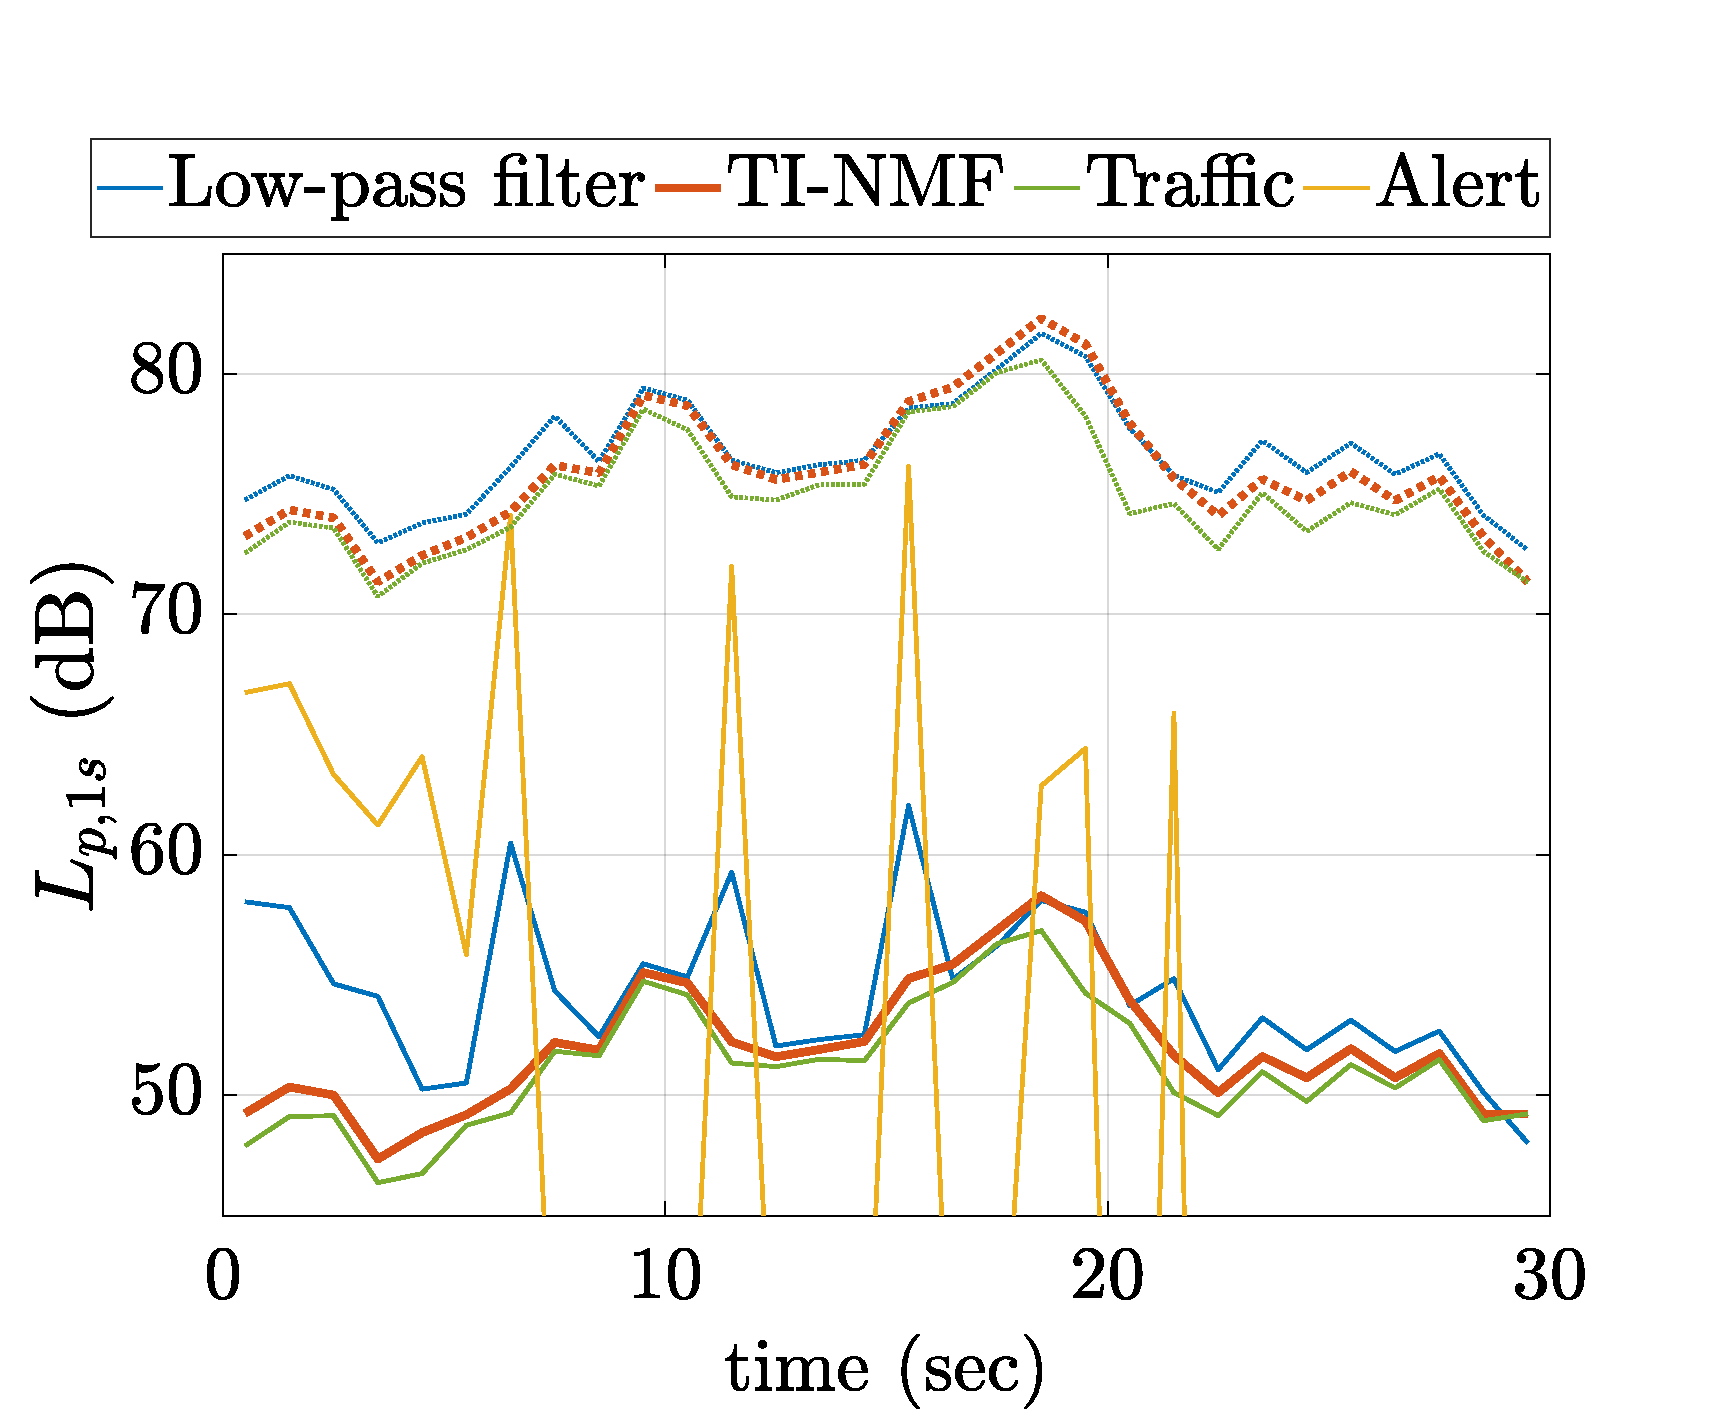
\includegraphics[width=\textwidth]{figures/NMF_Lp_alert.pdf}
%DIFDELCMD <  %%%
%DIFDELCMD < \caption{%
{%DIFAUXCMD
\DIFdelFL{1 second equivalent sound pressure level of an }\textit{\DIFdelFL{alert}} %DIFAUXCMD
\DIFdelFL{sub-class scene for 500 Hz low-pass filter and TI-NMF (\mbox{%DIFAUXCMD
$\beta$
}%DIFAUXCMD
= 1, \mbox{%DIFAUXCMD
$K$
}%DIFAUXCMD
= 200, \mbox{%DIFAUXCMD
$w_t$
}%DIFAUXCMD
= 0.5 s, \mbox{%DIFAUXCMD
$t$
}%DIFAUXCMD
= 0.42) at \mbox{%DIFAUXCMD
$TIR = -12$
}%DIFAUXCMD
dB (in full line) and \mbox{%DIFAUXCMD
$TIR$
}%DIFAUXCMD
= 12 dB (in dashed line).}}
	%DIFAUXCMD
%DIFDELCMD < \label{fig:lp_alert}
%DIFDELCMD < 
\end{figure}
%DIFDELCMD < 

%DIFDELCMD < \begin{figure*}[t]
%DIFDELCMD <   \centering
%DIFDELCMD <   \subfloat[$MAE$ error for each $TIR$ and sub-class with the frequency low-pass filter with $f_c$ = 500 Hz.]{\label{fig:TIR_class_filter}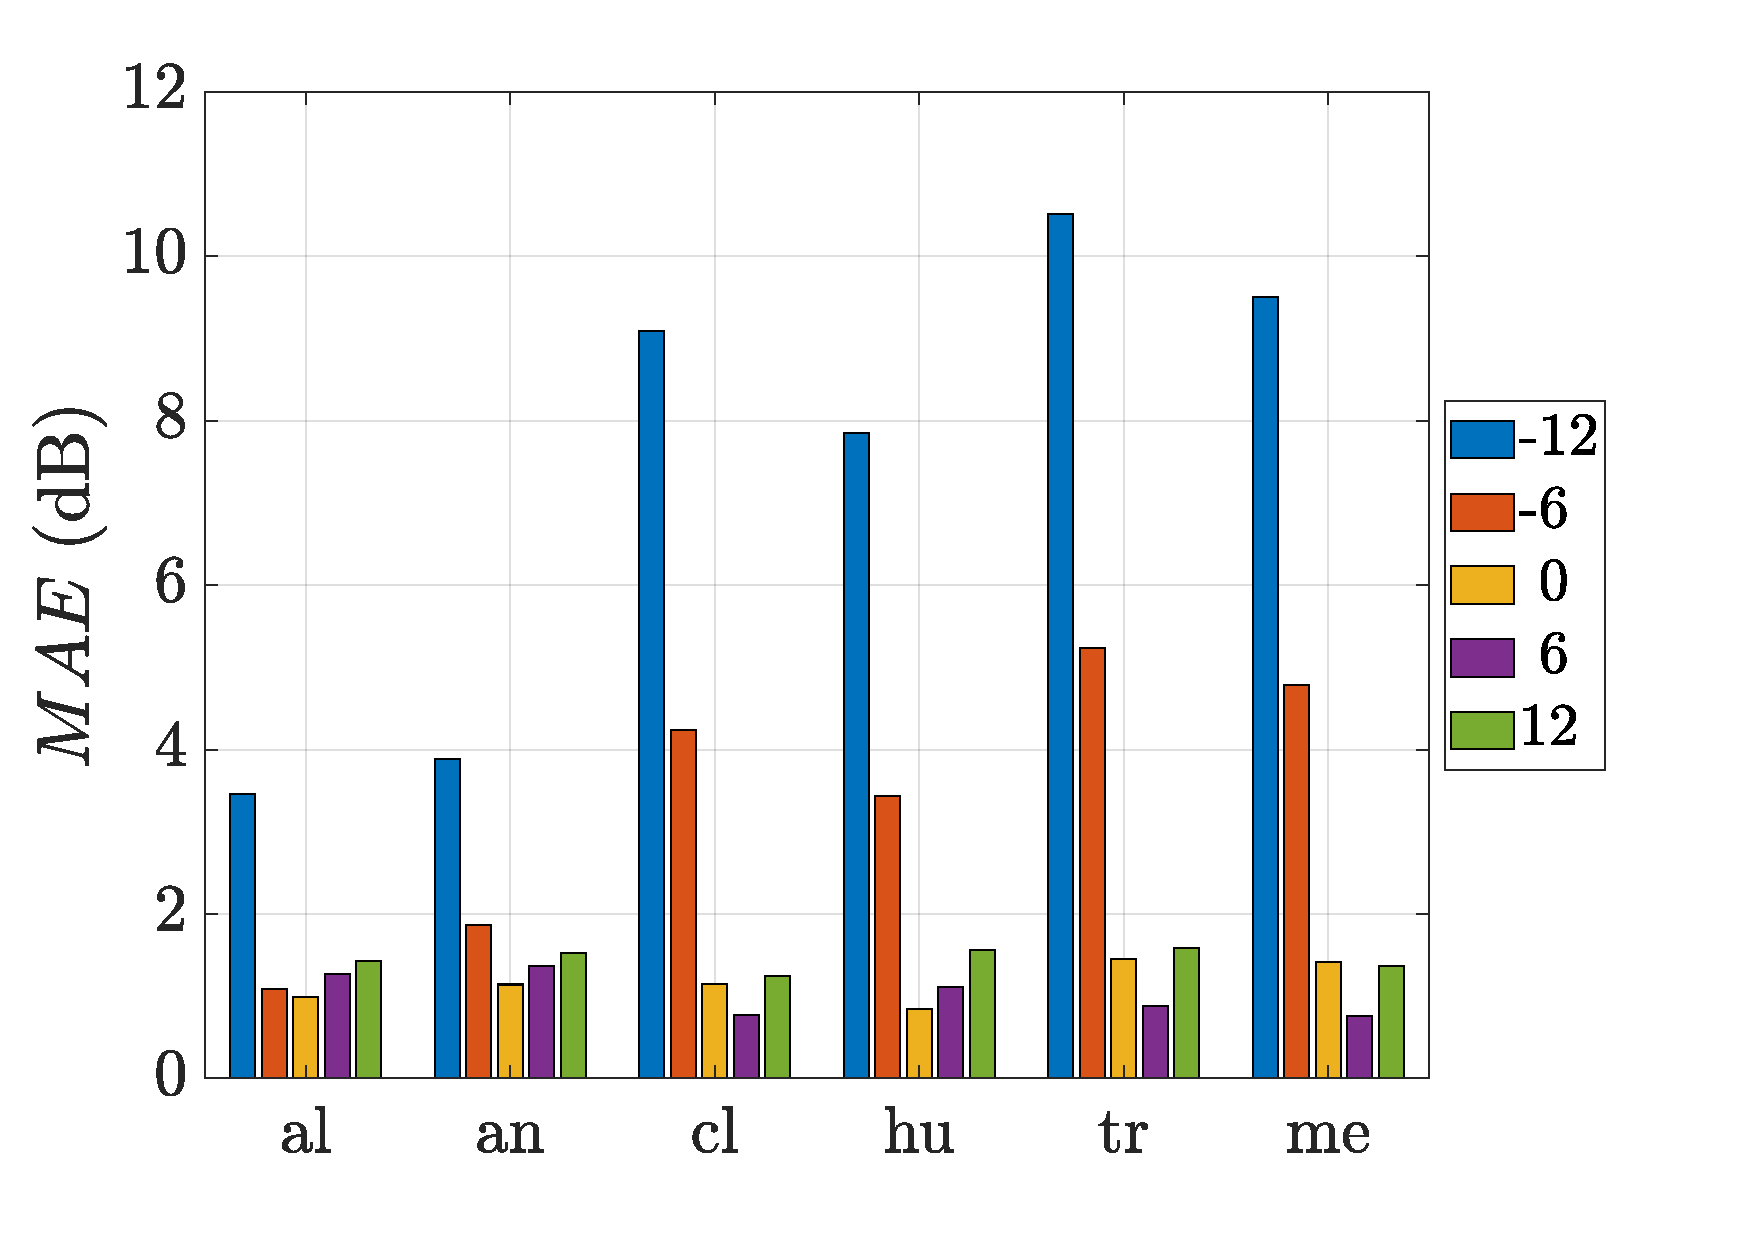
\includegraphics[width=0.45\textwidth]{figures/filter_bar.pdf}}
%DIFDELCMD <   %%%
\DIFdelFL{\hspace{5pt}
  }%DIFDELCMD < \subfloat[$MAE$ error for each $TIR$ and sub-class with Sup-NMF and $\beta$ = 2.]{\label{fig:TIR_class_sup}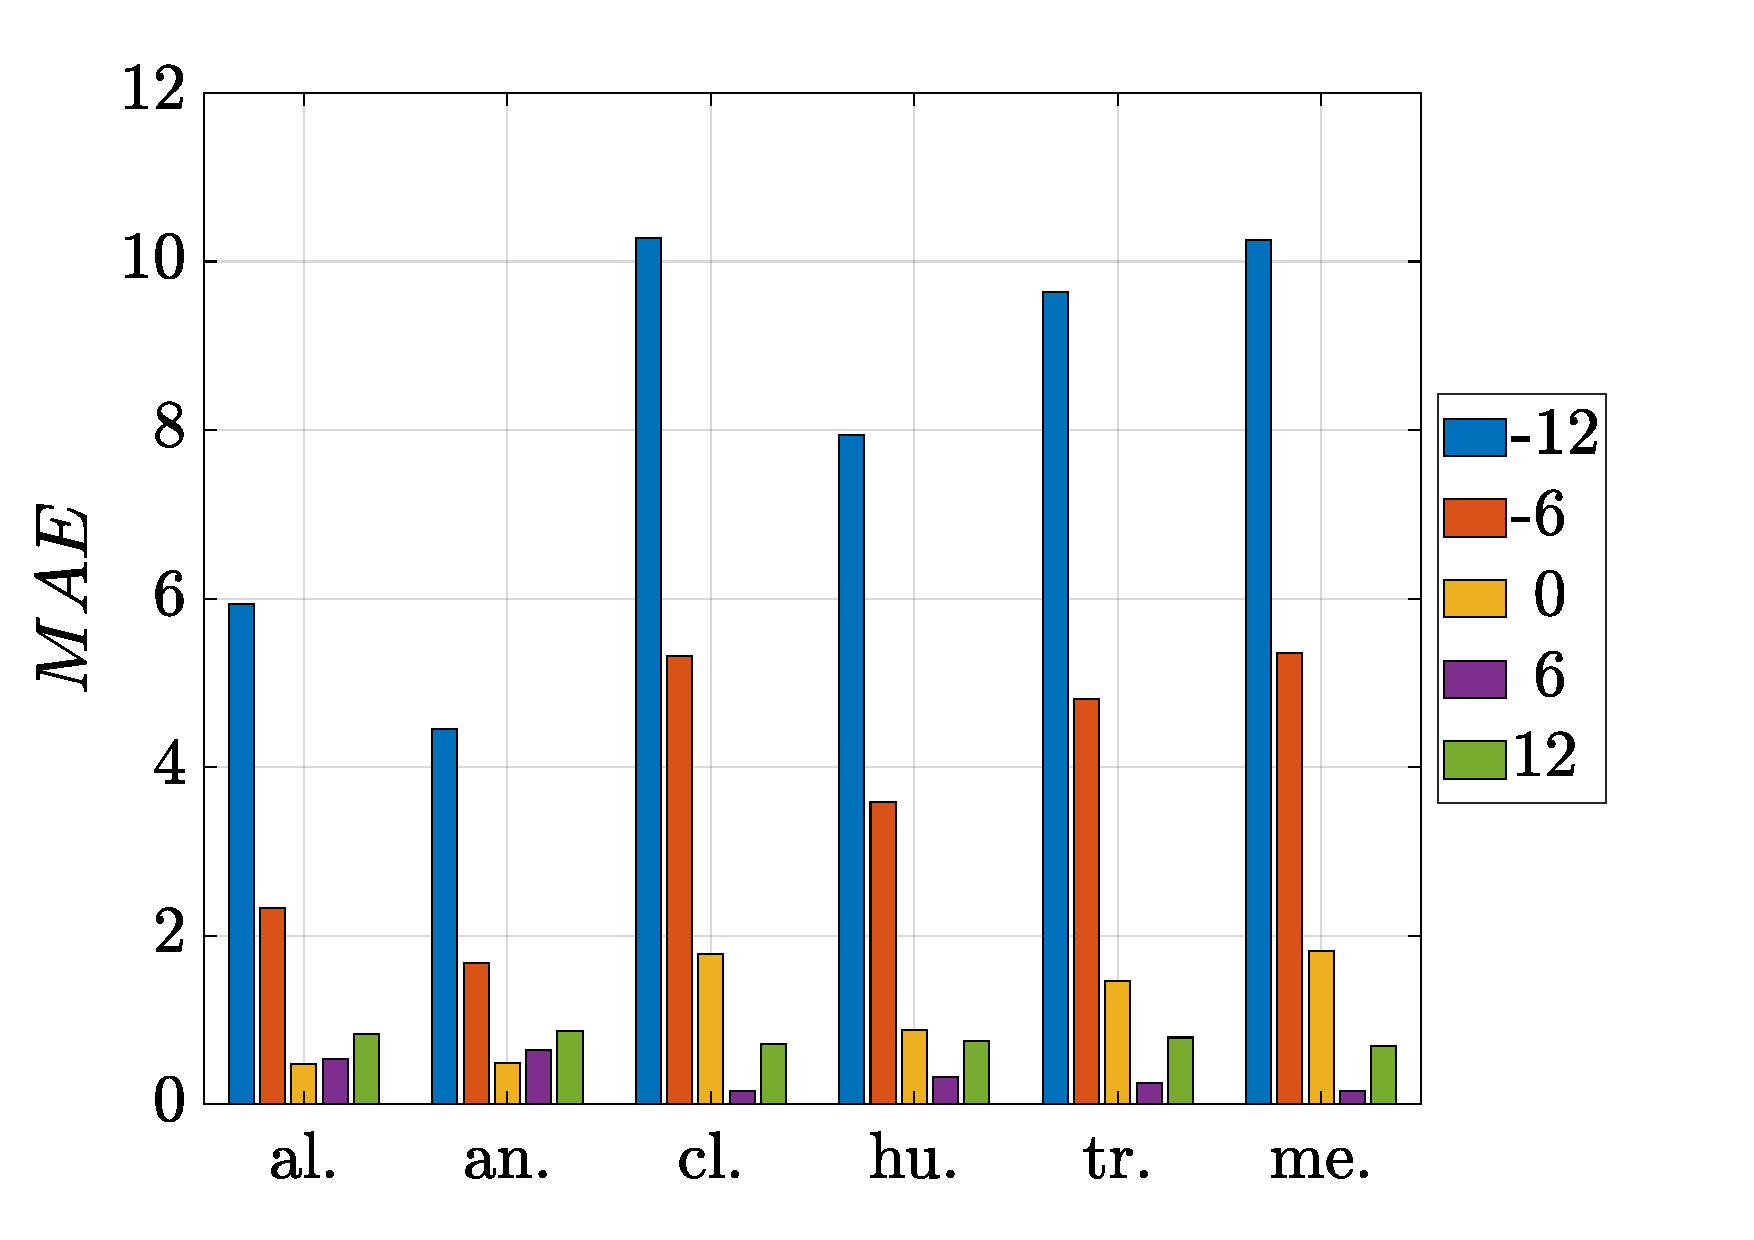
\includegraphics[width=0.45\linewidth]{figures/sup_bar.pdf}}
%DIFDELCMD <   %%%
\DIFdelFL{\hspace{5pt}
  }%DIFDELCMD < \subfloat[$MAE$ error for each $TIR$ and sub-class with Sem-NMF and $\beta$ = 2.]{\label{fig:TIR_class_semi}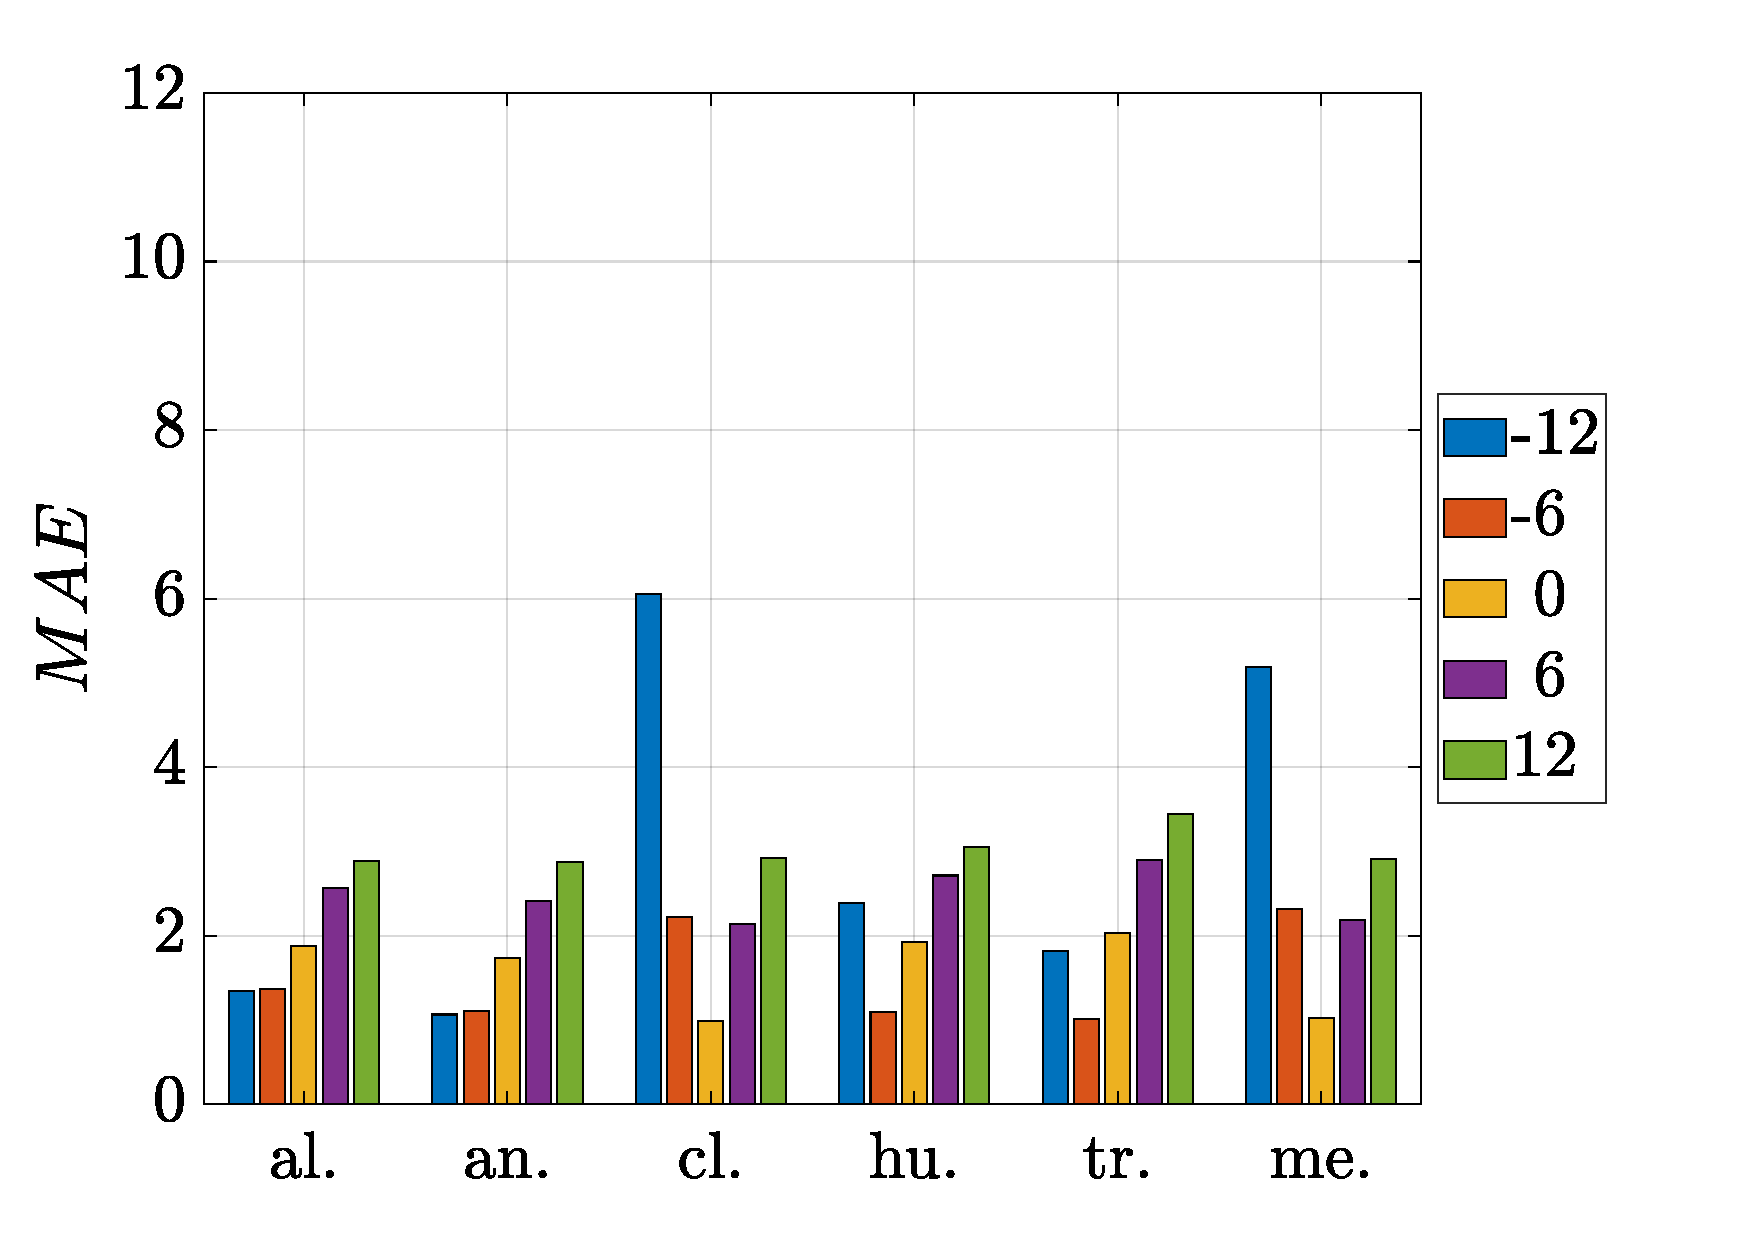
\includegraphics[width=.45\linewidth]{figures/semi-sup_bar.pdf}}
%DIFDELCMD <   %%%
\DIFdelFL{\hspace{5pt}
  }%DIFDELCMD < \subfloat[$MAE$ error for each $TIR$ and sub-class with TI-NMF, $\beta$ = 1 and $t$ = 0.42.]{\label{fig:TIR_class_TI}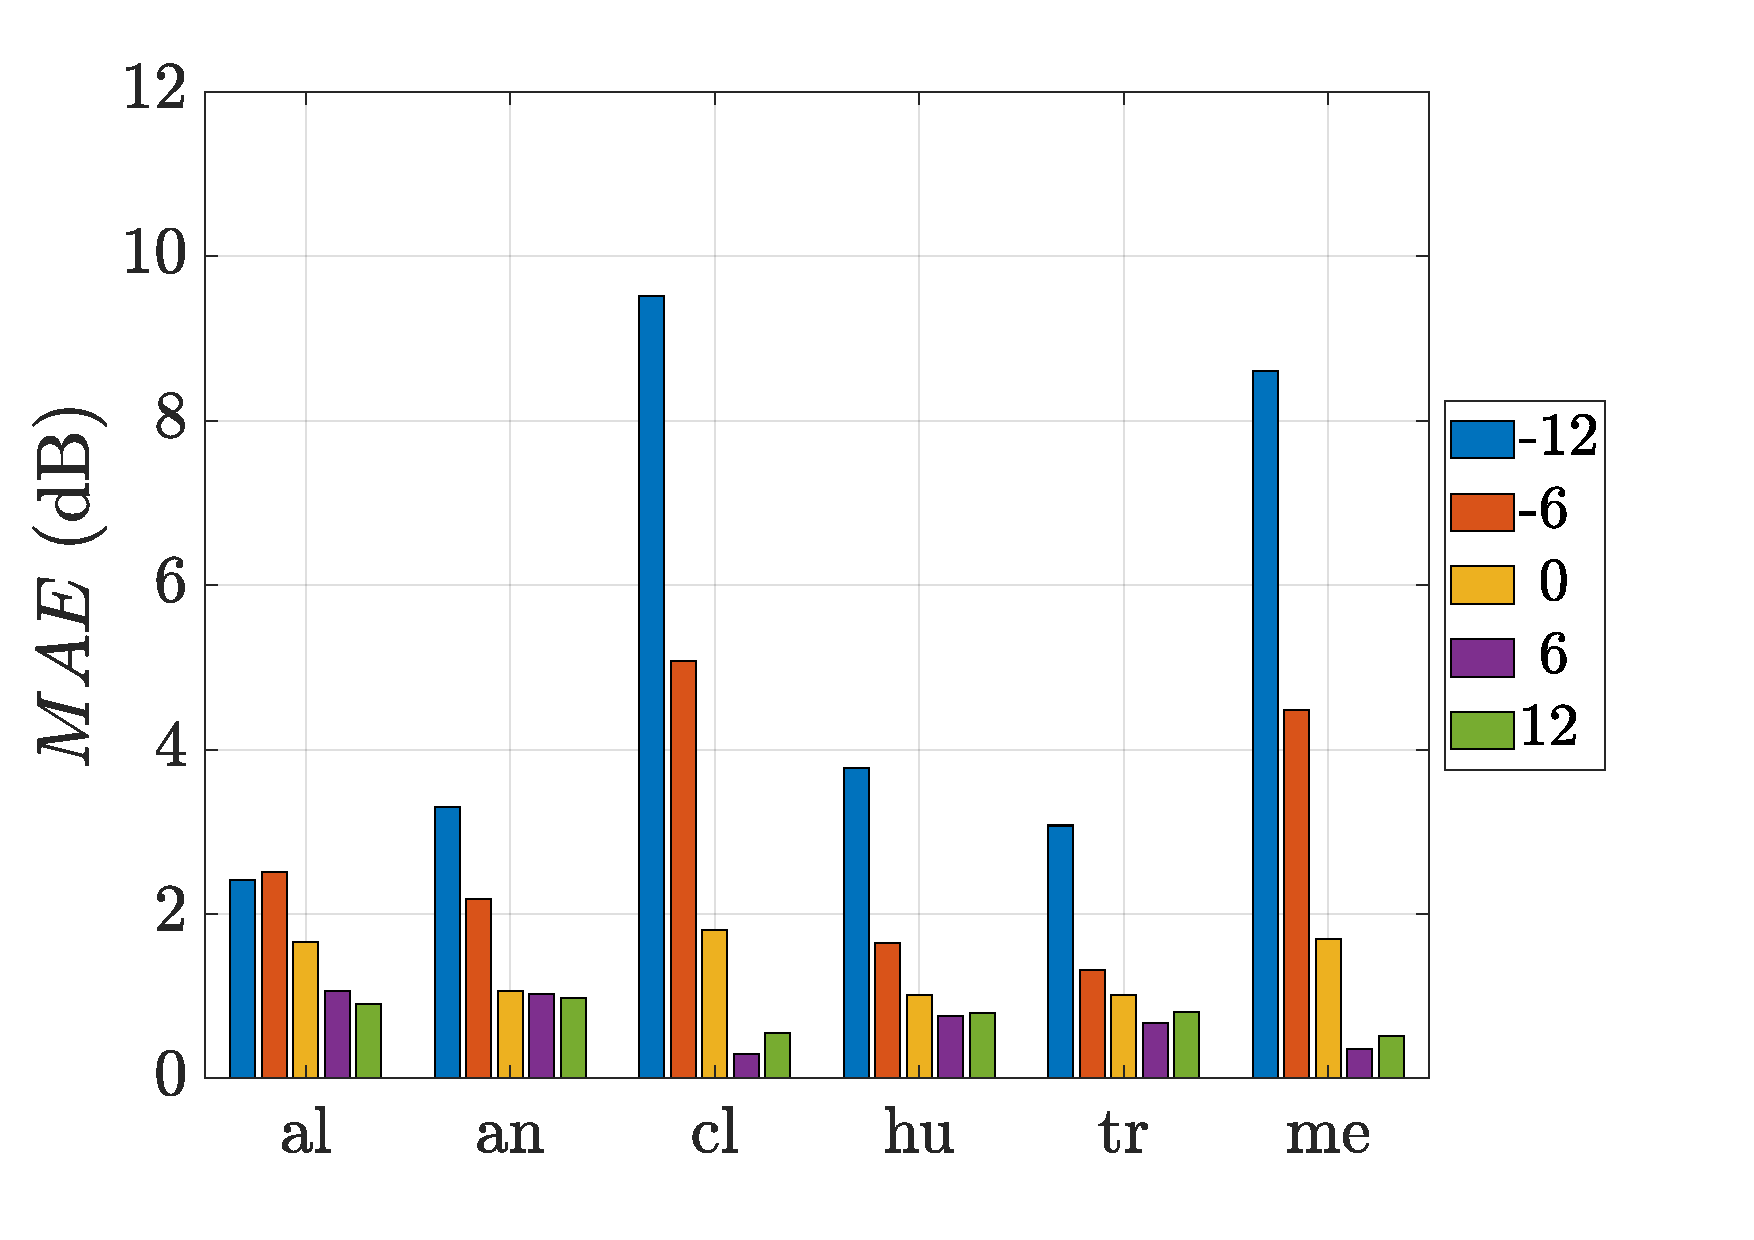
\includegraphics[width=.45\linewidth]{figures/TI_bar}}
%DIFDELCMD <   %%%
%DIFDELCMD < \caption{%
{%DIFAUXCMD
\DIFdelFL{\mbox{%DIFAUXCMD
$MAE$
}%DIFAUXCMD
(dB) error for each sub-class and each \mbox{%DIFAUXCMD
$TIR$
}%DIFAUXCMD
according to the the best results with the filter (\ref{fig:TIR_class_filter}) and each method (Sup-NMF (\ref{fig:TIR_class_sup}), Sem-NMF (\ref{fig:TIR_class_semi}) and TI-NMF (\ref{fig:TIR_class_TI})).}}
	%DIFAUXCMD
%DIFDELCMD < \label{fig:TIR_bar}
%DIFDELCMD < \end{figure*}
%DIFDELCMD < %%%
\DIFdelend \DIFaddbegin \DIFadd{The \mbox{%DIFAUXCMD
$MAE$
}%DIFAUXCMD
is a performance index without dimension. The use of such a metric is justified by the aim of this study that is to find the best association of experimental factors that obtains the lower mean error on all the corpus. The \mbox{%DIFAUXCMD
$MAE$
}%DIFAUXCMD
error with logarithmic values gives an equal weight to each difference for any given sound level and makes it possible to be less sensitive to errors in high pressure levels (in accordance with human perception). It is also a common practice in the environmental acoustics field when dealing with errors  \mbox{%DIFAUXCMD
\cite{morillas2014uncertainty} }%DIFAUXCMD
\mbox{%DIFAUXCMD
\cite{aumond2018kriging}}%DIFAUXCMD
.
}\DIFaddend 

\section{Results}\label{part:results}

\DIFdelbegin \DIFdel{Table \ref{tab:results} summarizes, according to the 2 main factors (}\textit{\DIFdel{method}}%DIFAUXCMD
\DIFdel{, \mbox{%DIFAUXCMD
$\beta$
}%DIFAUXCMD
), the lowest \mbox{%DIFAUXCMD
$MAE$
}%DIFAUXCMD
error averaged on all sub-classes and all \mbox{%DIFAUXCMD
$TIR$
}%DIFAUXCMD
(750 sound mixtures in all). For the low-pass frequency filters and each NMF approaches, the best parameter combinations are detailed according to the \mbox{%DIFAUXCMD
$TIR$
}%DIFAUXCMD
in Table \ref{tab:results_TIR},  and are expanded to the sub-classes in Figures \ref{fig:TIR_class_filter}, \ref{fig:TIR_class_sup}, \ref{fig:TIR_class_semi} and \ref{fig:TIR_class_TI}.
}%DIFDELCMD < \\
%DIFDELCMD < %%%
\DIFdelend \DIFaddbegin 
\begin{figure}
[t]
\centering
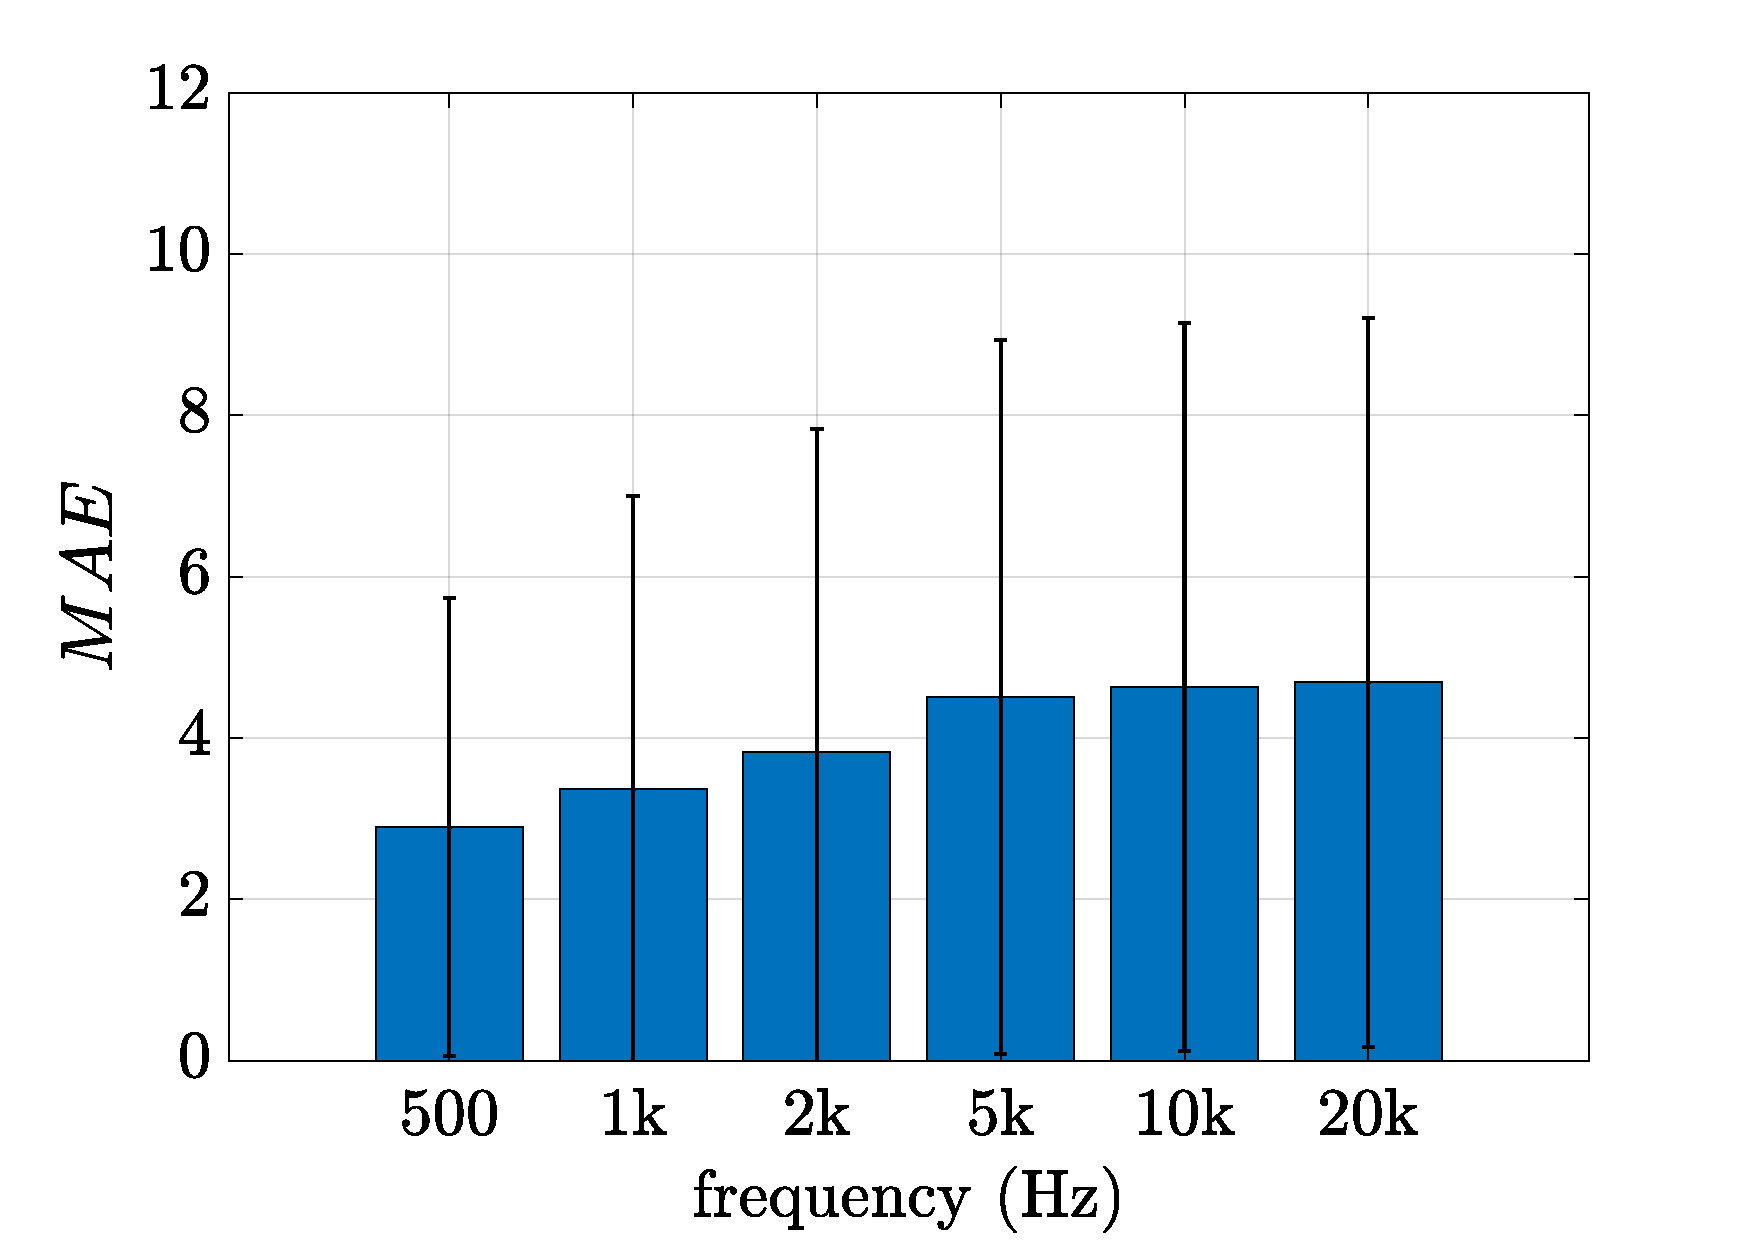
\includegraphics[width=\linewidth]{./figures/filter_bar_integrate.pdf}
\caption{\DIFaddFL{Average \mbox{%DIFAUXCMD
$MAE$
}%DIFAUXCMD
errors for the LP filter on all the corpus.}}
\label{fig:filter_intergate}
\end{figure}
\DIFaddend 


First, the errors \DIFdelbegin \DIFdel{produced by the filter are detailed. }\DIFdelend \DIFaddbegin \DIFadd{calculated from the traffic sound estimation of the low-pass filter on all the corpus are detailed in Figure \ref{fig:filter_intergate}. The LP filter with the cut-off frequency }\DIFaddend $f_c = 20 $ kHz \DIFaddbegin \DIFadd{generates the highest error as it }\DIFaddend is equivalent to consider all the sound \DIFdelbegin \DIFdel{mixtures }\DIFdelend \DIFaddbegin \DIFadd{mixture }\DIFaddend without distinction between traffic and others sound sources. Consequently, \DIFaddbegin \DIFadd{on Table \ref{tab:results_TIR} }\DIFaddend in low $TIR$ (-12 dB and -6 dB), where traffic component is scarce, the error is more important than \DIFdelbegin \DIFdel{in }\DIFdelend \DIFaddbegin \DIFadd{for }\DIFaddend high $TIR$ (6 dB and 12 dB) where the traffic component is predominant. \DIFdelbegin \DIFdel{\mbox{%DIFAUXCMD
$f_c = 500$
}%DIFAUXCMD
Hz is }\DIFdelend \DIFaddbegin \DIFadd{Even if the performances for the positive \mbox{%DIFAUXCMD
$TIR$
}%DIFAUXCMD
values are high, it has to be reminded that in practice, the \mbox{%DIFAUXCMD
$TIR$
}%DIFAUXCMD
value is not known. In consequence, without any prior knowledge, this approach cannot be applied. The traffic sound level estimation error decrease with }\DIFaddend the cut-off frequency\DIFdelbegin \DIFdel{with }\DIFdelend \DIFaddbegin \DIFadd{. Finally, \mbox{%DIFAUXCMD
$f_c = 500$
}%DIFAUXCMD
Hz is the one which reach }\DIFaddend the lowest mean error obtained (\DIFaddbegin \DIFadd{\mbox{%DIFAUXCMD
$MAE$
}%DIFAUXCMD
= }\DIFaddend 2.89 ($\pm$ 2.84)\DIFdelbegin \DIFdel{dB}\DIFdelend ). It is then considered as the baseline to compare the performances of NMF.

In low $TIR$, for \textit{alert} and \textit{animals}, which are sub-classes composed of higher frequencies, this filter is efficient as it removes these frequency components. For the other sub-classes where low frequency contents are present (storm for \textit{climate}, voices in \textit{humans}, planes, tramway and train in \textit{transport} and ventilation noise in \textit{mechanics}), the filter considers all the energy located in the pass-band and then does not dissociate the traffic element from the other sound sources. The errors are then nearly all superior to 4 \DIFdelbegin \DIFdel{dB and are }\DIFdelend \DIFaddbegin \DIFadd{as the traffic level is }\DIFaddend overestimated. In opposite, in high $TIR$, the error is due to the energy removed from the traffic which has the consequence to underestimate the sound levels. The 500 Hz filter finds a balance between what is put aside in low $TIR$ and what it is remained in high $TIR$. \\

\DIFaddbegin \DIFadd{Table \ref{tab:results} summarizes, according to the 2 main factors (}\textit{\DIFadd{method}}\DIFadd{, \mbox{%DIFAUXCMD
$\beta$
}%DIFAUXCMD
), the lowest \mbox{%DIFAUXCMD
$MAE$
}%DIFAUXCMD
error averaged on all sub-classes and all \mbox{%DIFAUXCMD
$TIR$
}%DIFAUXCMD
(750 sound mixtures in all) for NMF. For the low-pass frequency filters and each NMF approaches, the best parameter combinations are detailed according to the \mbox{%DIFAUXCMD
$TIR$
}%DIFAUXCMD
in Table \ref{tab:results_TIR},  and are expanded to the sub-classes in Figures \ref{fig:TIR_class_filter}, \ref{fig:TIR_class_sup}, \ref{fig:TIR_class_semi} and \ref{fig:TIR_class_TI}. }\DIFaddend Compared with the filter errors, the choice of some NMF approaches makes it possible to decrease the error of the road traffic sound level estimation. The supervised approach is the only method that has an average error superior to the 500 Hz filter baseline. Sem-NMF and TI-NMF have better results. The lowest average error is obtained for TI-NMF,  \DIFdelbegin \DIFdel{2.19 }\DIFdelend \DIFaddbegin \DIFadd{2.15 }\DIFaddend ($\pm$ \DIFdelbegin \DIFdel{2.18)dB}\DIFdelend \DIFaddbegin \DIFadd{2.10)}\DIFaddend , for $\beta$ = 1 and threshold $t$ = \DIFdelbegin \DIFdel{0.42 }\DIFdelend \DIFaddbegin \DIFadd{0.41 }\DIFaddend with the dictionary factors $K$ = 200 and $w_t$ = 500 ms. On the other hand, the semi-supervised approach has a higher error but a lower standard deviation (\DIFaddbegin \DIFadd{\mbox{%DIFAUXCMD
$MAE$
}%DIFAUXCMD
= }\DIFaddend 2.32 ($\pm$ \DIFdelbegin \DIFdel{1.26)dB). }\DIFdelend \DIFaddbegin \DIFadd{1.15)). TI-NMF seems to be the most efficient approach on all corpus without requiring strong prior knowledge about the interfering sound class or the \mbox{%DIFAUXCMD
$TIR$
}%DIFAUXCMD
value.
}\DIFaddend 

\DIFdelbegin \DIFdel{According to Table \ref{tab:results_TIR} and Figures \ref{fig:TIR_bar}, the behavior between the 3 versions of NMF differs}\DIFdelend \DIFaddbegin \DIFadd{As the mean error between the best SUP-NMF (\mbox{%DIFAUXCMD
$\beta$
}%DIFAUXCMD
= 2, \mbox{%DIFAUXCMD
$K$
}%DIFAUXCMD
= 25, \mbox{%DIFAUXCMD
$w_t$
}%DIFAUXCMD
= 2 s), SEM-NMF (\mbox{%DIFAUXCMD
$\beta$
}%DIFAUXCMD
= 1, \mbox{%DIFAUXCMD
$K$
}%DIFAUXCMD
= 200, \mbox{%DIFAUXCMD
$w_t$
}%DIFAUXCMD
= 2 s) and TI-NMF (\mbox{%DIFAUXCMD
$\beta$
}%DIFAUXCMD
= 1, \mbox{%DIFAUXCMD
$K$
}%DIFAUXCMD
= 200, \mbox{%DIFAUXCMD
$w_t$
}%DIFAUXCMD
= 0.5 s, \mbox{%DIFAUXCMD
$t$
}%DIFAUXCMD
= 0.41) approaches are close, a Student's t-test is performed to evaluate the statistical differences between them. It is performed on the 750 estimated traffic sound levels for each couple of methods (SUP/SEM NMF, SUP/TI NMF, SEM/TI NMF). The test estimates the \mbox{%DIFAUXCMD
$p$
}%DIFAUXCMD
-value which is confronted to a threshold \mbox{%DIFAUXCMD
$\alpha$
}%DIFAUXCMD
= 5 \mbox{%DIFAUXCMD
$\%$
}%DIFAUXCMD
. The \mbox{%DIFAUXCMD
$p$
}%DIFAUXCMD
-values are summarized in the Table \ref{tab:student_test} with the \mbox{%DIFAUXCMD
$t$
}%DIFAUXCMD
-values and the degrees of freedom (Dof).
}

\begin{table}
[t]
\centering
\begin{tabular}{lccccc}
\toprule
  & \DIFaddFL{SUP/SEM NMF }& \DIFaddFL{SUP/TI NMF }& \DIFaddFL{SEM/TI NMF }\\
\midrule
\DIFaddFL{t-test }& \DIFaddFL{Welch }& \DIFaddFL{Welch }& \DIFaddFL{Student }\\
\DIFaddFL{\mbox{%DIFAUXCMD
$t$
}%DIFAUXCMD
-value }& \DIFaddFL{7.81 }& \DIFaddFL{2.84 }& \DIFaddFL{4.60}\\
\DIFaddFL{Dof }& \DIFaddFL{1478 }& \DIFaddFL{1470 }& \DIFaddFL{1498}\\
\DIFaddFL{\mbox{%DIFAUXCMD
$p$
}%DIFAUXCMD
-value }& \textbf{\DIFaddFL{1.06 \mbox{%DIFAUXCMD
$\times 10^{-14}$
}%DIFAUXCMD
}} & \textbf{\DIFaddFL{4.49 \mbox{%DIFAUXCMD
$\times 10^{-3}$
}%DIFAUXCMD
}} & \textbf{\DIFaddFL{4.39 \mbox{%DIFAUXCMD
$\times 10^{-6}$
}%DIFAUXCMD
}} \\
\bottomrule
\end{tabular}
\caption{\DIFaddFL{\mbox{%DIFAUXCMD
$p$
}%DIFAUXCMD
-values deducted from the paired sample one-sided t-test of the SUP , SEM and TI NMF that offer the lowest \mbox{%DIFAUXCMD
$MAE$
}%DIFAUXCMD
error. In bold letters, the \mbox{%DIFAUXCMD
$p$
}%DIFAUXCMD
-values that reject the \mbox{%DIFAUXCMD
$H_0$
}%DIFAUXCMD
hypothesis (\mbox{%DIFAUXCMD
$p$
}%DIFAUXCMD
-value \mbox{%DIFAUXCMD
$\leq \alpha$
}%DIFAUXCMD
).}}
\label{tab:student_test}
\end{table}
\DIFadd{For each couple of methods, the \mbox{%DIFAUXCMD
$H_0$
}%DIFAUXCMD
hypothesis is rejected meaning that the distributions of the sound level estimations according to the approaches are significantly different despite similar mean errors}\DIFaddend . In the case of \DIFdelbegin \DIFdel{Sup-NMF, it fails to improve the filtering performances despite good results in high \mbox{%DIFAUXCMD
$TIR$
}%DIFAUXCMD
. The errors are too important for low \mbox{%DIFAUXCMD
$TIR$
}%DIFAUXCMD
and this for all }\DIFdelend \DIFaddbegin \DIFadd{the comparison of the distributions of the SEM NMF with the TI NMF, a Student's t-test is calculated. But since the standard deviations are different between the SUP NMF and SEM NMF distributions and between the SUP NMF and TI NMF distributions, a Welch's t-test is performed, which is an adaptation of the Student's t-test. Consequently, the calculation of the degree of freedom is then obtained as a function of these variances and differs from that obtained by the Student t-test. To better understand these differences, the errors made according to }\DIFaddend the \DIFaddbegin \DIFadd{\mbox{%DIFAUXCMD
$TIR$
}%DIFAUXCMD
and for each sound environment are displayed in Table \ref{tab:results_TIR} and in Figure \ref{fig:TIR_bar}.
}

\begin{table*}[t]
\centering
\caption{\DIFaddFL{\mbox{%DIFAUXCMD
$MAE$
}%DIFAUXCMD
error averaged on all sub-classes on each \mbox{%DIFAUXCMD
$TIR$
}%DIFAUXCMD
for the best scenario according to each method.}}
\begin{tabular}{@{}cccccc@{}}
\toprule
\textbf{\DIFaddFL{method}} & \DIFaddFL{filter }& \DIFaddFL{filter }& \DIFaddFL{Sup-NMF }& \DIFaddFL{Sem-NMF }& \DIFaddFL{TI-NMF }\\ \midrule
\DIFaddFL{\mbox{%DIFAUXCMD
$f_c$
}%DIFAUXCMD
(kHz) }& \DIFaddFL{20 }& \DIFaddFL{0.5 }& \DIFaddFL{- }& \DIFaddFL{- }& \DIFaddFL{- }\\
\DIFaddFL{\mbox{%DIFAUXCMD
$\mathbf{\beta}$
}%DIFAUXCMD
}& \DIFaddFL{- }& \DIFaddFL{- }& \DIFaddFL{2 }& \DIFaddFL{2 }& \DIFaddFL{1 }\\ \hline
\textbf{\DIFaddFL{-12}} & \DIFaddFL{12.25 (\mbox{%DIFAUXCMD
$\pm$
}%DIFAUXCMD
0.05) }& \DIFaddFL{7.39 (\mbox{%DIFAUXCMD
$\pm$
}%DIFAUXCMD
3.00) }& \DIFaddFL{8.08 (\mbox{%DIFAUXCMD
$\pm$
}%DIFAUXCMD
2.44) }& \DIFaddFL{2.98 (\mbox{%DIFAUXCMD
$\pm$
}%DIFAUXCMD
2.11) }& \DIFaddFL{5.22 (\mbox{%DIFAUXCMD
$\pm$
}%DIFAUXCMD
2.62) }\\
\textbf{\DIFaddFL{-6}} & \DIFaddFL{6.96 (\mbox{%DIFAUXCMD
$\pm$
}%DIFAUXCMD
0.05) }& \DIFaddFL{3.44 (\mbox{%DIFAUXCMD
$\pm$
}%DIFAUXCMD
1.65) }& \DIFaddFL{3.84 (\mbox{%DIFAUXCMD
$\pm$
}%DIFAUXCMD
1.58) }& \DIFaddFL{1.52 (\mbox{%DIFAUXCMD
$\pm$
}%DIFAUXCMD
0.60)  }& \DIFaddFL{2.72 (\mbox{%DIFAUXCMD
$\pm$
}%DIFAUXCMD
1.24) }\\
\textbf{\DIFaddFL{0}} & \DIFaddFL{3.00 (\mbox{%DIFAUXCMD
$\pm$
}%DIFAUXCMD
0.03) }& \DIFaddFL{1.17 (\mbox{%DIFAUXCMD
$\pm$
}%DIFAUXCMD
0.24) }& \DIFaddFL{1.15 (\mbox{%DIFAUXCMD
$\pm$
}%DIFAUXCMD
0.62) }& \DIFaddFL{1.60 (\mbox{%DIFAUXCMD
$\pm$
}%DIFAUXCMD
0.47) }& \DIFaddFL{1.26 (\mbox{%DIFAUXCMD
$\pm$
}%DIFAUXCMD
0.35) }\\
\textbf{\DIFaddFL{6}} & \DIFaddFL{0.97 (\mbox{%DIFAUXCMD
$\pm$
}%DIFAUXCMD
0.01) }& \DIFaddFL{1.03 (\mbox{%DIFAUXCMD
$\pm$
}%DIFAUXCMD
0.26) }& \DIFaddFL{0.35 (\mbox{%DIFAUXCMD
$\pm$
}%DIFAUXCMD
0.20) }& \DIFaddFL{2.49 (\mbox{%DIFAUXCMD
$\pm$
}%DIFAUXCMD
0.30) }& \DIFaddFL{0.75 (\mbox{%DIFAUXCMD
$\pm$
}%DIFAUXCMD
0.34) }\\
\textbf{\DIFaddFL{12}} & \DIFaddFL{0.26 (\mbox{%DIFAUXCMD
$\pm$
}%DIFAUXCMD
0.00) }& \DIFaddFL{1.45 (\mbox{%DIFAUXCMD
$\pm$
}%DIFAUXCMD
0.13) }& \DIFaddFL{0.77 (\mbox{%DIFAUXCMD
$\pm$
}%DIFAUXCMD
0.07) }& \DIFaddFL{3.02 (\mbox{%DIFAUXCMD
$\pm$
}%DIFAUXCMD
0.22) }& \DIFaddFL{0.83 (\mbox{%DIFAUXCMD
$\pm$
}%DIFAUXCMD
0.23) }\\ \bottomrule
\end{tabular}
\label{tab:results_TIR}
\end{table*}

\begin{figure*}[t]
  \centering
  \subfloat[\mbox{%DIFAUXCMD
$MAE$
}%DIFAUXCMD
error for each \mbox{%DIFAUXCMD
$TIR$
}%DIFAUXCMD
and sub-class with the frequency low-pass filter with \mbox{%DIFAUXCMD
$f_c$
}%DIFAUXCMD
= 500 Hz.]{\label{fig:TIR_class_filter}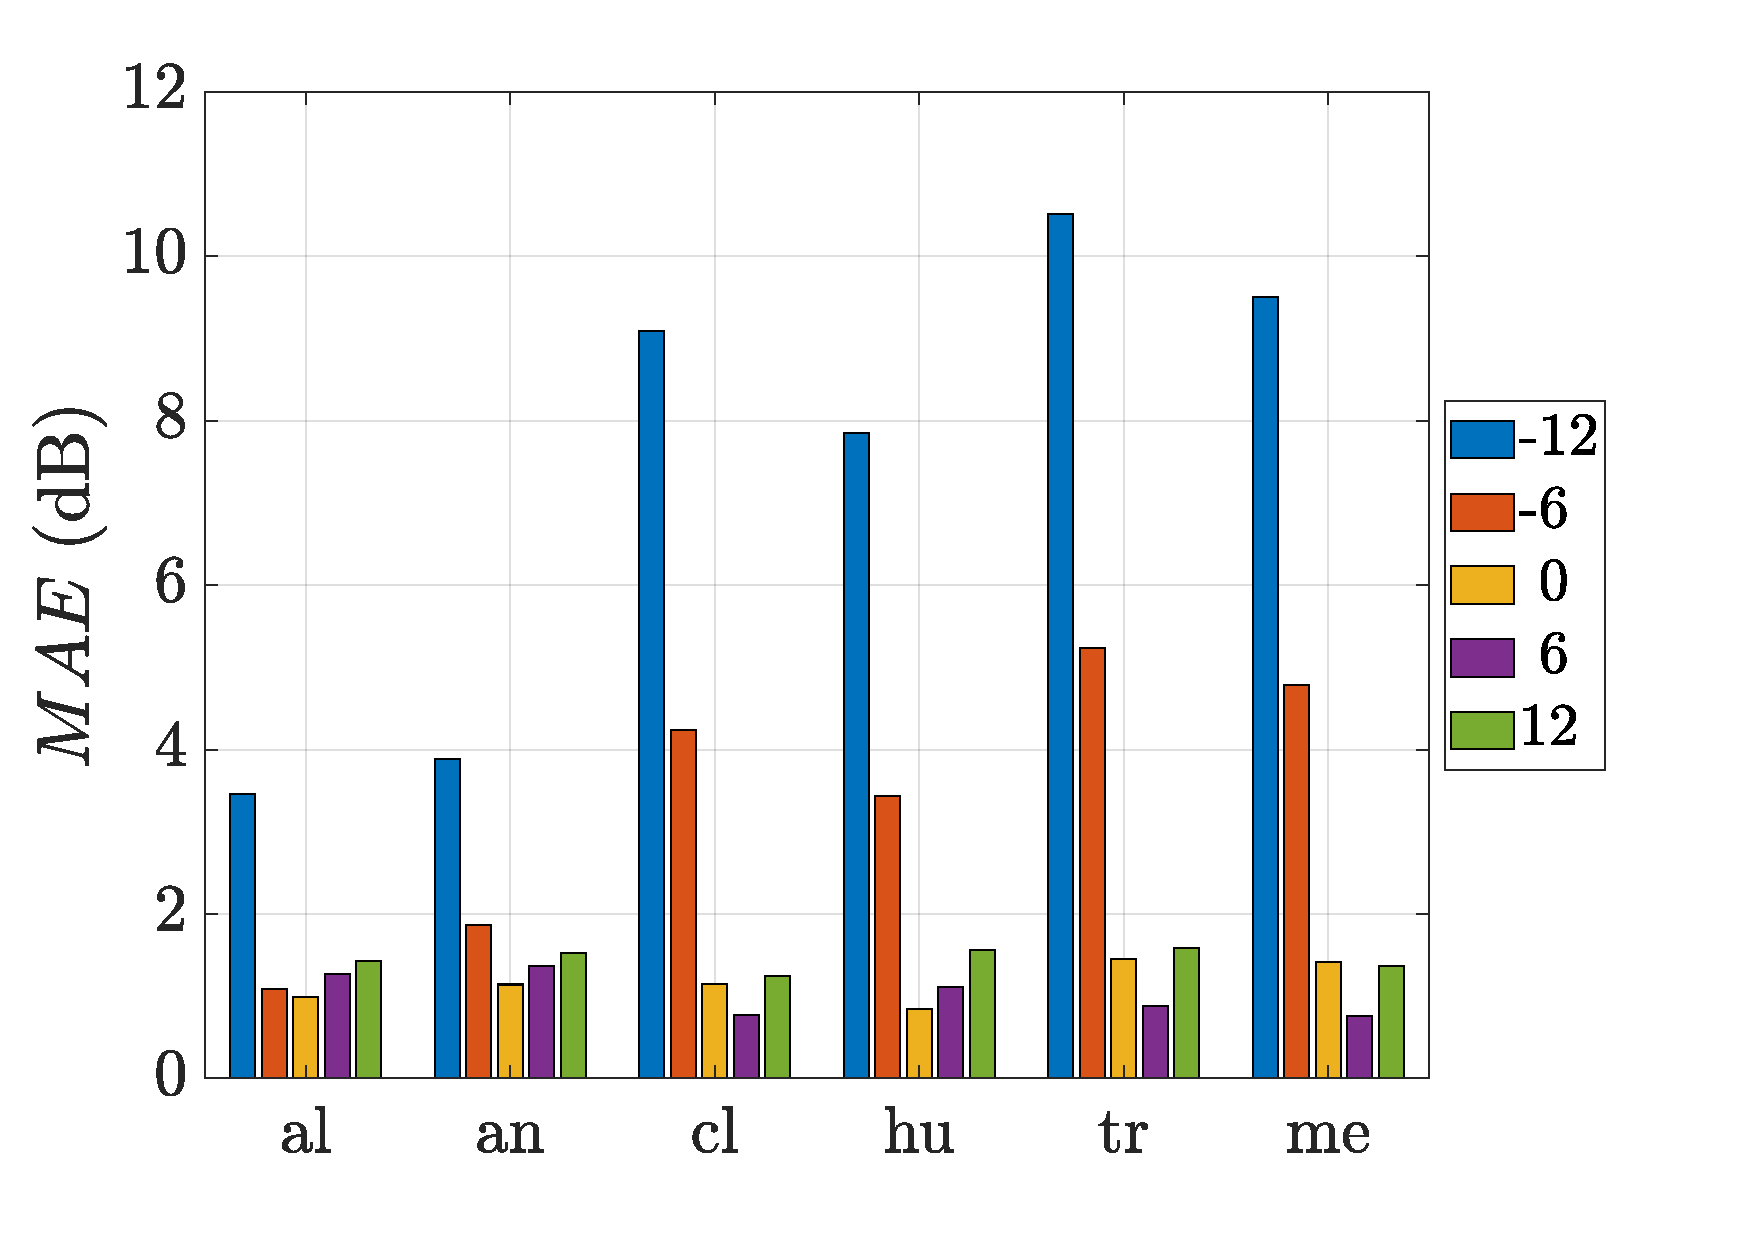
\includegraphics[width=0.45\textwidth]{figures/filter_bar.pdf}}
  \DIFaddFL{\hspace{5pt}
  }\subfloat[\mbox{%DIFAUXCMD
$MAE$
}%DIFAUXCMD
error for each \mbox{%DIFAUXCMD
$TIR$
}%DIFAUXCMD
and sub-class with Sup-NMF and \mbox{%DIFAUXCMD
$\beta$
}%DIFAUXCMD
= 2.]{\label{fig:TIR_class_sup}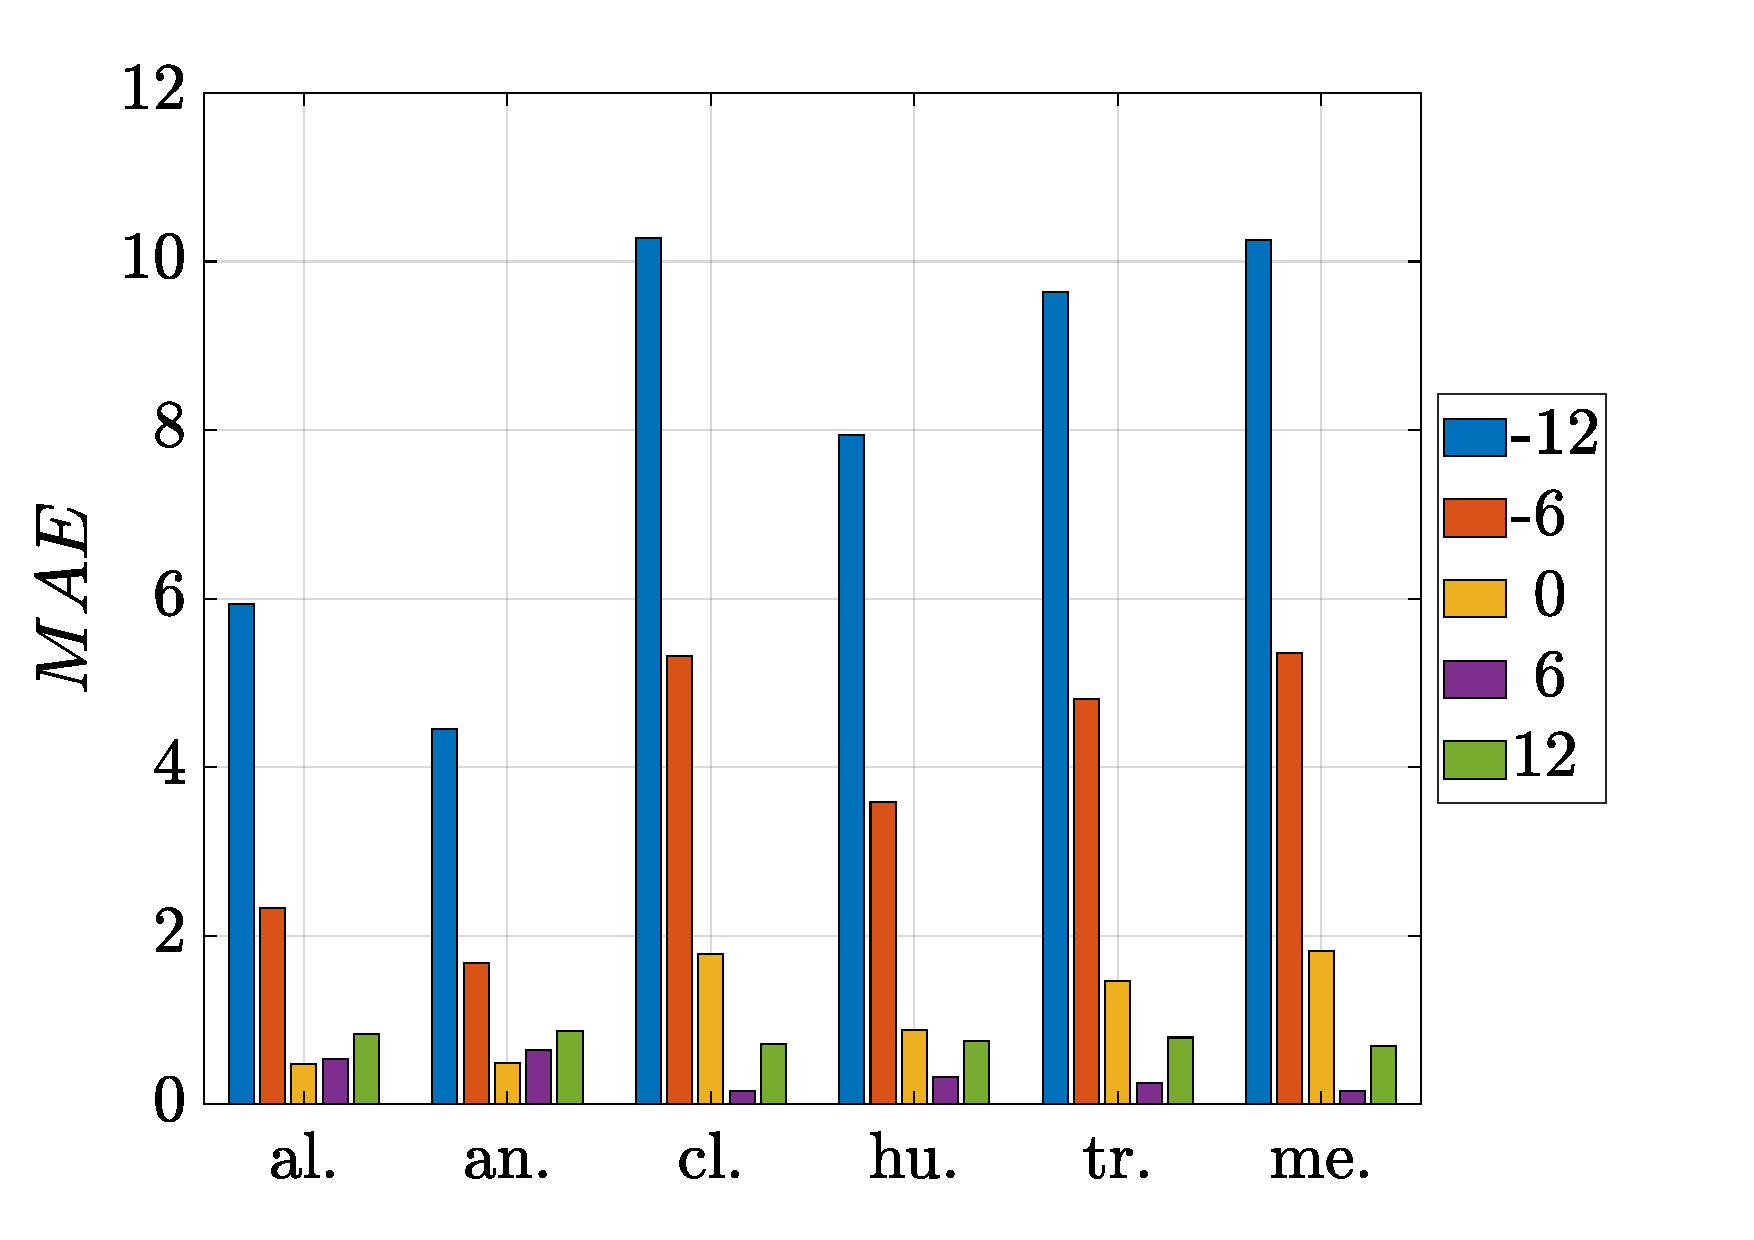
\includegraphics[width=0.45\linewidth]{figures/sup_bar.pdf}}
  \DIFaddFL{\hspace{5pt}
  }\subfloat[\mbox{%DIFAUXCMD
$MAE$
}%DIFAUXCMD
error for each \mbox{%DIFAUXCMD
$TIR$
}%DIFAUXCMD
and sub-class with Sem-NMF and \mbox{%DIFAUXCMD
$\beta$
}%DIFAUXCMD
= 1.]{\label{fig:TIR_class_semi}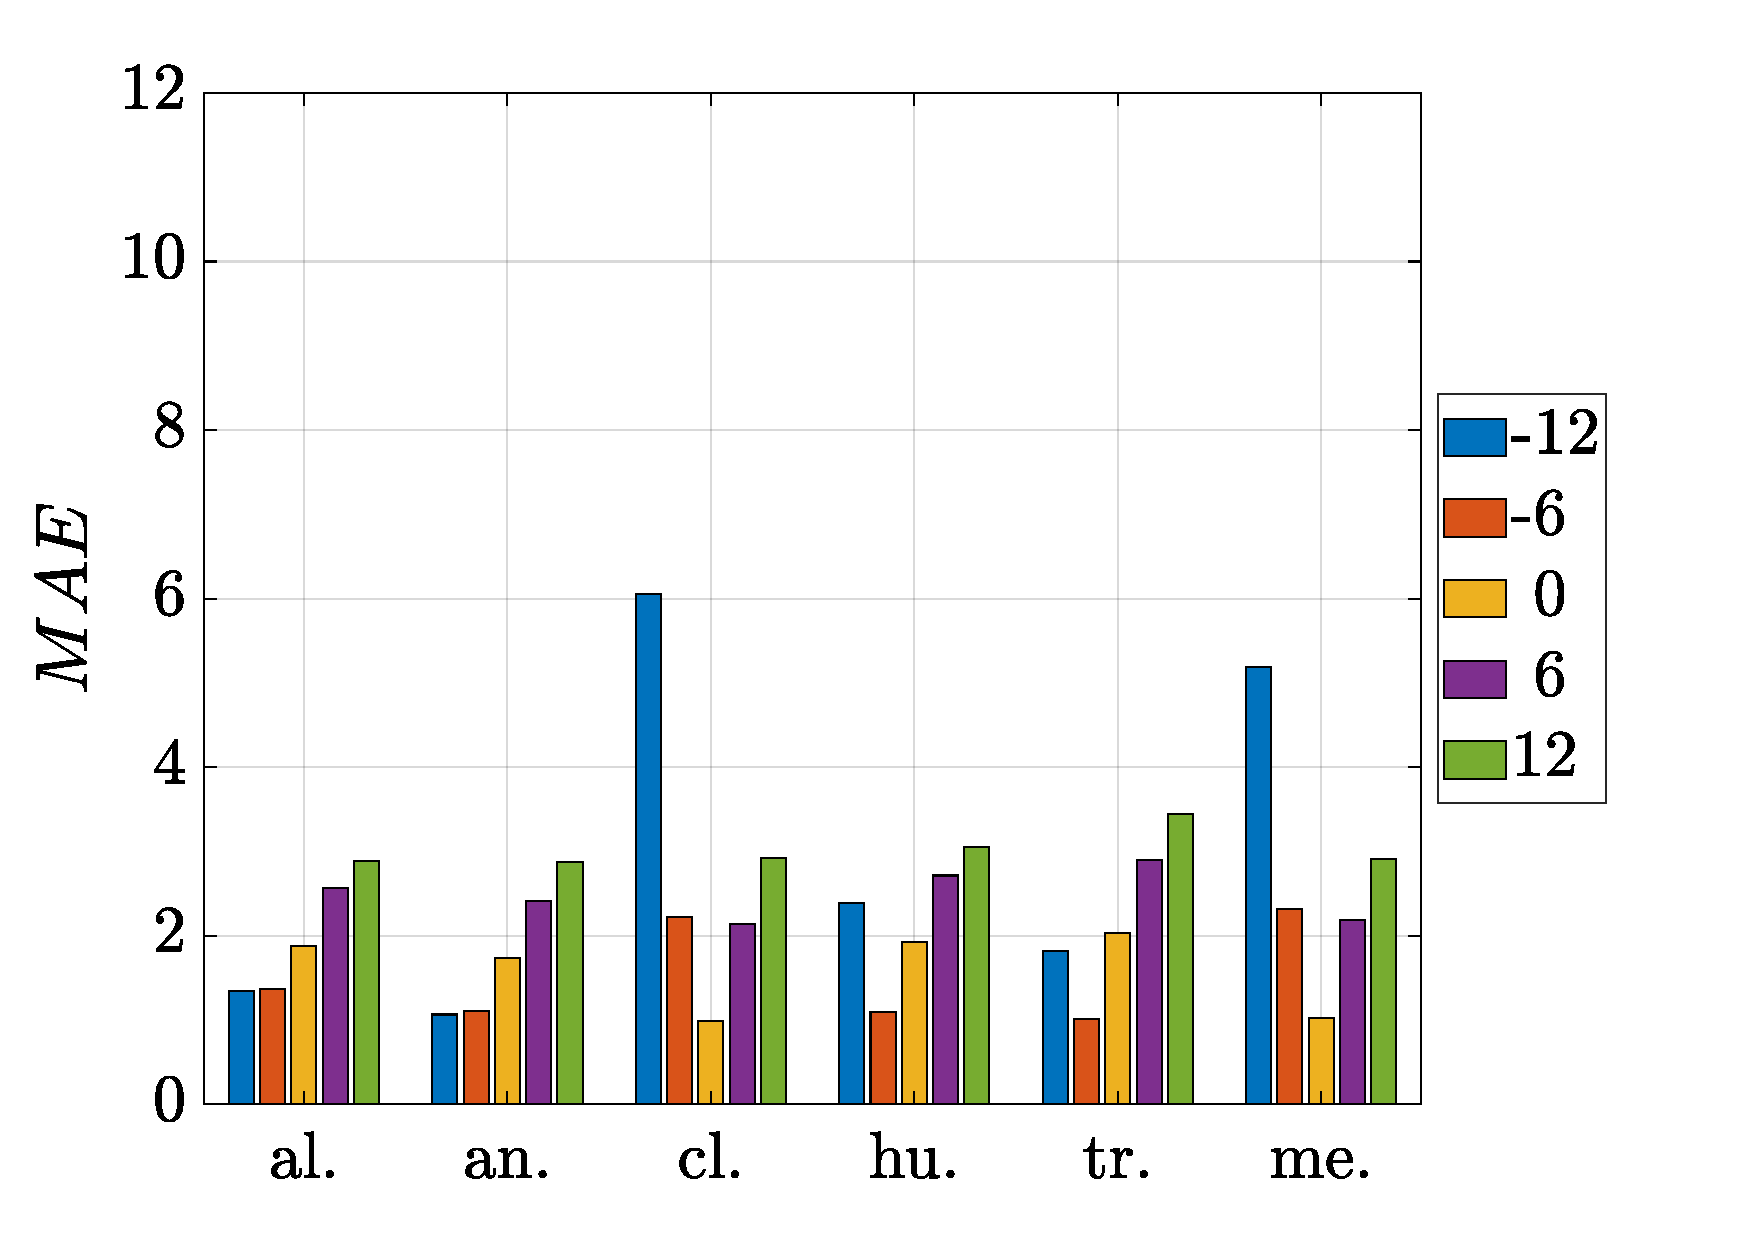
\includegraphics[width=.45\linewidth]{figures/semi-sup_bar.pdf}}
  \DIFaddFL{\hspace{5pt}
  }\subfloat[\mbox{%DIFAUXCMD
$MAE$
}%DIFAUXCMD
error for each \mbox{%DIFAUXCMD
$TIR$
}%DIFAUXCMD
and sub-class with TI-NMF, \mbox{%DIFAUXCMD
$\beta$
}%DIFAUXCMD
= 1 and \mbox{%DIFAUXCMD
$t$
}%DIFAUXCMD
= 0.41.]{\label{fig:TIR_class_TI}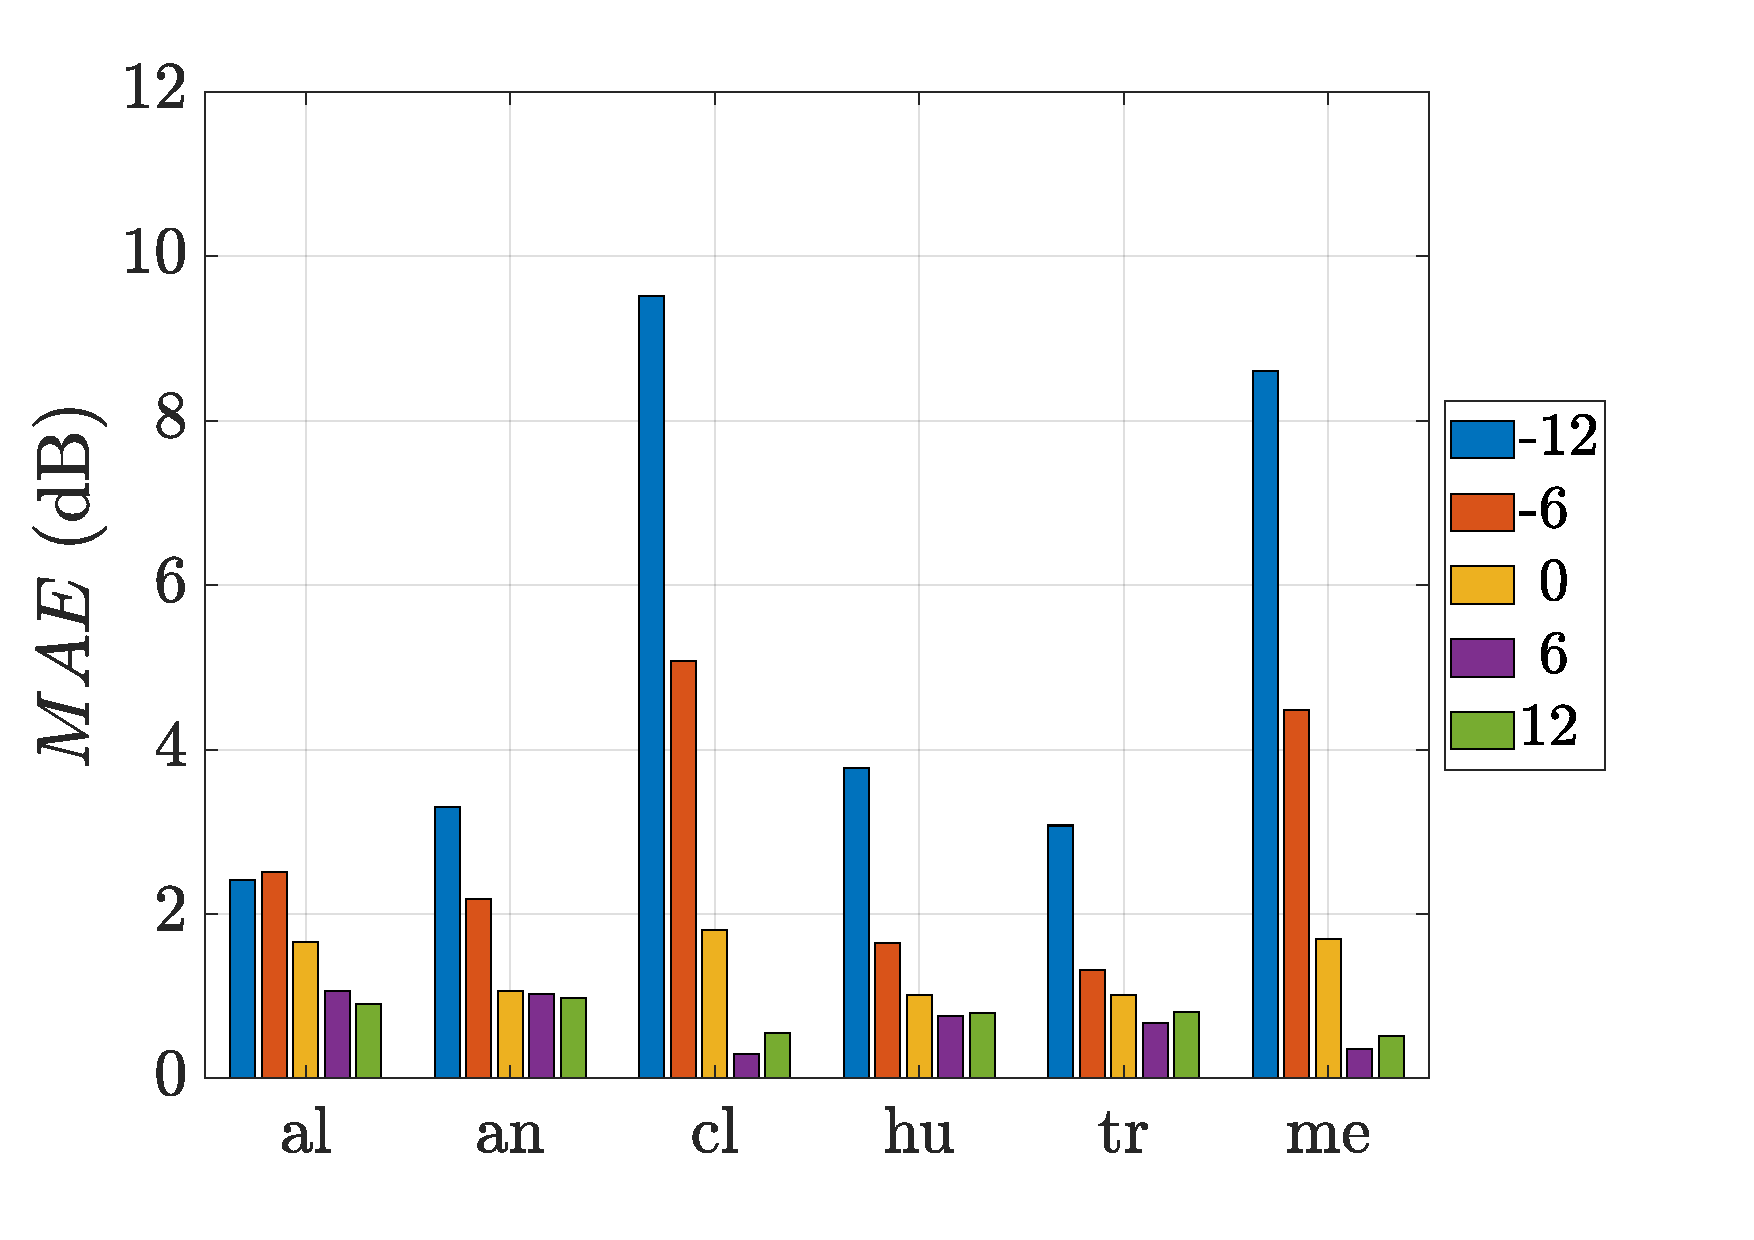
\includegraphics[width=.45\linewidth]{figures/TI_bar}}
  \caption{\DIFaddFL{\mbox{%DIFAUXCMD
$MAE$
}%DIFAUXCMD
(dB) error for each sub-class and each \mbox{%DIFAUXCMD
$TIR$
}%DIFAUXCMD
according to the best results with the filter (\ref{fig:TIR_class_filter}) and each method (Sup-NMF (\ref{fig:TIR_class_sup}), Sem-NMF (\ref{fig:TIR_class_semi}) and TI-NMF (\ref{fig:TIR_class_TI})).}}
	\label{fig:TIR_bar}
\end{figure*}

\DIFadd{In the case of Sup-NMF, the \mbox{%DIFAUXCMD
$MAE$
}%DIFAUXCMD
errors are important for all }\DIFaddend sub-classes \DIFdelbegin \DIFdel{. This method }\DIFdelend \DIFaddbegin \DIFadd{at low \mbox{%DIFAUXCMD
$TIR$
}%DIFAUXCMD
. This approach }\DIFaddend reveals to be too rigid as $\mathbf{W}$ is composed of fixed traffic spectra. In the \DIFdelbegin \DIFdel{case of low \mbox{%DIFAUXCMD
$TIR$
}%DIFAUXCMD
, in the }\DIFdelend aim to reduce the objective function, see eq. \ref{eq:min-D-WH}, traffic elements are used whatever the sound event in the sound scene. Thus forcing the dictionary to be only \DIFaddbegin \DIFadd{composed of }\DIFaddend traffic spectra is not a sufficient way to estimate correctly the traffic sound level, $\tilde{L}_{p,traffic}$. \DIFaddbegin \DIFadd{At high \mbox{%DIFAUXCMD
$TIR$
}%DIFAUXCMD
, this approach generates better estimations as it is a favorable case: the }\textit{\DIFadd{traffic}} \DIFadd{is the main component with a dictionary dedicated to this sound source.
}\DIFaddend 

\DIFdelbegin \DIFdel{Consequently, with }\DIFdelend \DIFaddbegin \DIFadd{With }\DIFaddend the addition of a mobile part in the dictionary, $\mathbf{W_r}$, the semi-supervised approach allows \DIFdelbegin \DIFdel{a better consideration of }\DIFdelend \DIFaddbegin \DIFadd{us to better take into account }\DIFaddend the interfering class in low $TIR$. It \DIFaddbegin \DIFadd{thus }\DIFaddend brings a significant decrease of the errors for low $TIR$. However, the relatively high degrees of freedom of Sem-NMF are restrictive for high $TIR$ as the errors exceed 2 dB for all sub-classes and increase with $TIR \in \lbrace$6, 12$\rbrace$ dB. \DIFaddbegin \DIFadd{The performances are even superior to the LP filter baseline. }\DIFaddend In order to reduce $D(\mathbf{V} \vert \vert \mathbf{WH}$), without constraint, Sem-NMF is free to include traffic components in $\mathbf{W_r}$. Consequently, this behavior decreases the quality of the reconstruction of the traffic component.

\DIFdelbegin \DIFdel{Finally, }\DIFdelend \DIFaddbegin \DIFadd{The }\DIFaddend TI-NMF \DIFaddbegin \DIFadd{behavior, }\DIFaddend with a threshold \DIFdelbegin \DIFdel{\mbox{%DIFAUXCMD
$t = 0.42$
}%DIFAUXCMD
}\DIFdelend \DIFaddbegin \DIFadd{\mbox{%DIFAUXCMD
$t = 0.41$
}%DIFAUXCMD
}\DIFaddend and $\beta$ = 1, \DIFdelbegin \DIFdel{offers the lowest average error (Table \ref{tab:results})}\DIFdelend \DIFaddbegin \DIFadd{generates smaller errors compared to the baseline for all the \mbox{%DIFAUXCMD
$TIR$
}%DIFAUXCMD
values, with the exception at \mbox{%DIFAUXCMD
$TIR$
}%DIFAUXCMD
= 0 dB. If this approach gives the lowest error on all the corpus, it is not the one that propose on each \mbox{%DIFAUXCMD
$TIR$
}%DIFAUXCMD
the best performances: SUP-NMF has lower errors for positive \mbox{%DIFAUXCMD
$TIR$
}%DIFAUXCMD
while SEM-NMF surpasses it for \mbox{%DIFAUXCMD
$TIR \in \left\lbrace -12, -6\right\rbrace$
}%DIFAUXCMD
. But the specific case \mbox{%DIFAUXCMD
$TIR = -12 dB$
}%DIFAUXCMD
is a less likely limit case in urban environment. Putting this specific case aside, TI-NMF is the only approach that propose an error inferior to 3 dB for \mbox{%DIFAUXCMD
$TIR \in \left\lbrace -6, 12 \right\rbrace$
}%DIFAUXCMD
dB}\DIFaddend . Unlike Sup-NMF, where $\mathbf{W}$ is fixed, and Sem-NMF, where only $\mathbf{W_r}$ is updated, TI-NMF updates $\mathbf{W}$ entirely to adjust prior knowledge to the scene under evaluation so as to adapt to the different sound environments. The closest elements of the traffic component defined in $\mathbf{W_0}$ are then extracted to deduce the traffic signal.
\DIFaddbegin 

\DIFaddend For low $TIR$, as the traffic sound class is not predominant, the final dictionary \DIFaddbegin \DIFadd{\mbox{%DIFAUXCMD
$\mathbf{W'}$
}%DIFAUXCMD
}\DIFaddend strongly differs from \DIFdelbegin \DIFdel{the }\DIFdelend $\mathbf{W_0}$. With the thresholding, only a reduced number of basis vectors are considered as traffic components\DIFaddbegin \DIFadd{: from the 200 basis contained in \mbox{%DIFAUXCMD
$\mathbf{W'}$
}%DIFAUXCMD
, 106 are considered as }\textit{\DIFadd{traffic}}  \DIFadd{component in \mbox{%DIFAUXCMD
$TIR$
}%DIFAUXCMD
= -12 dB}\DIFaddend . In comparison to supervised results, this approach reduces significantly the error for the \textit{human} and \textit{transport} sub-classes.  However, for \textit{climate} and \textit{mechanics}, the errors remain important as these interfering classes have similar spectral profiles when compared to traffic ones. 

For high $TIR$, as the traffic is the main sound source, the similarity of the initial dictionary and $\mathbf{W}$ is higher which allows \DIFdelbegin \DIFdel{retaining }\DIFdelend \DIFaddbegin \DIFadd{us to retain }\DIFaddend more elements as traffic components \DIFaddbegin \DIFadd{(181 basis for \mbox{%DIFAUXCMD
$TIR$
}%DIFAUXCMD
= 12 dB) }\DIFaddend and then decreases the error (\DIFaddbegin \DIFadd{\mbox{%DIFAUXCMD
$MAE$
}%DIFAUXCMD
}\DIFaddend < 1\DIFdelbegin \DIFdel{dB}\DIFdelend ). The kept elements are then more suited to the scenes than a fixed dictionary. The error for these $TIR$ is then due to the thresholding which put aside some elements that \DIFdelbegin \DIFdel{are nevertheless }\DIFdelend \DIFaddbegin \DIFadd{can be }\DIFaddend related to the traffic component.
\DIFdelbegin \DIFdel{In Figure \ref{fig:lp_alert}, the 1 second equivalent sound pressure level of an alert scene is displayed for \mbox{%DIFAUXCMD
$TIR \in \lbrace -12,12 \rbrace$
}%DIFAUXCMD
dB for the 500 Hz low pass filter and for TI-NMF. In the case of \mbox{%DIFAUXCMD
$TIR=-12$
}%DIFAUXCMD
dB, the traffic elements selected in TI-NMF do not activated when the alarm class sounds contrary to the low-pass filter.
}\DIFdelend 

\DIFdelbegin \DIFdel{With a low threshold, it is }\DIFdelend \DIFaddbegin \DIFadd{It would be }\DIFaddend possible to decrease the error \DIFdelbegin \DIFdel{. For }\DIFdelend \DIFaddbegin \DIFadd{by adapting the threshold according to the \mbox{%DIFAUXCMD
$TIR$
}%DIFAUXCMD
. For instance at }\DIFaddend $TIR$ = 12 dB, the average error on all the sub-classes \DIFdelbegin \DIFdel{is 0.22 }\DIFdelend \DIFaddbegin \DIFadd{would decrease to 0.30 }\DIFaddend ($\pm$ \DIFdelbegin \DIFdel{0.08) dB }\DIFdelend \DIFaddbegin \DIFadd{0.11) }\DIFaddend with $t$ = \DIFdelbegin \DIFdel{0.30. In opposite for }\DIFdelend \DIFaddbegin \DIFadd{0.34 where 191 elements are considered as traffic component. On contrary, at }\DIFaddend $TIR$ = -12 dB, \DIFdelbegin \DIFdel{it is better to choose a high threshold \mbox{%DIFAUXCMD
$t$
}%DIFAUXCMD
= 0.55}\DIFdelend \DIFaddbegin \DIFadd{by increasing the threshold to 0.53}\DIFaddend , the error \DIFdelbegin \DIFdel{decrease then to 4.46 }\DIFdelend \DIFaddbegin \DIFadd{would decrease to 4.49 }\DIFaddend ($\pm$ \DIFdelbegin \DIFdel{1.66) dB.
In }\DIFdelend \DIFaddbegin \DIFadd{1.75) with in average 73 elements considered as }\textit{\DIFadd{traffic}} \DIFadd{elements.
}

\DIFadd{But, in }\DIFaddend order to generalize this method \DIFaddbegin \DIFadd{to a practical case }\DIFaddend where no prior knowledge on the urban environment \DIFaddbegin \DIFadd{is available}\DIFaddend , the chosen threshold $t$ is then fixed to $t$ = \DIFdelbegin \DIFdel{0.42 }\DIFdelend \DIFaddbegin \DIFadd{0.41 }\DIFaddend as it is the one that best \DIFdelbegin \DIFdel{balanced }\DIFdelend \DIFaddbegin \DIFadd{balance }\DIFaddend these opposite cases.
\DIFaddbegin \DIFadd{In Figure \ref{fig:specLp}, the spectrogram of an alert scene is displayed (\mbox{%DIFAUXCMD
$TIR$
}%DIFAUXCMD
= 0 dB). The evolution of the 1 second equivalent sound pressure level for \mbox{%DIFAUXCMD
$TIR \in \lbrace -12,12 \rbrace$
}%DIFAUXCMD
dB for the 500 Hz low pass filter and for TI-NMF can be seen on Figure \ref{fig:lp_alert}. In the case of \mbox{%DIFAUXCMD
$TIR=-12$
}%DIFAUXCMD
dB, the traffic elements selected in TI-NMF are not activated when the alarm class sounds contrary to the low-pass filter.
}


\begin{figure*}[t]
  \centering
  \subfloat[]{\label{fig:specLp}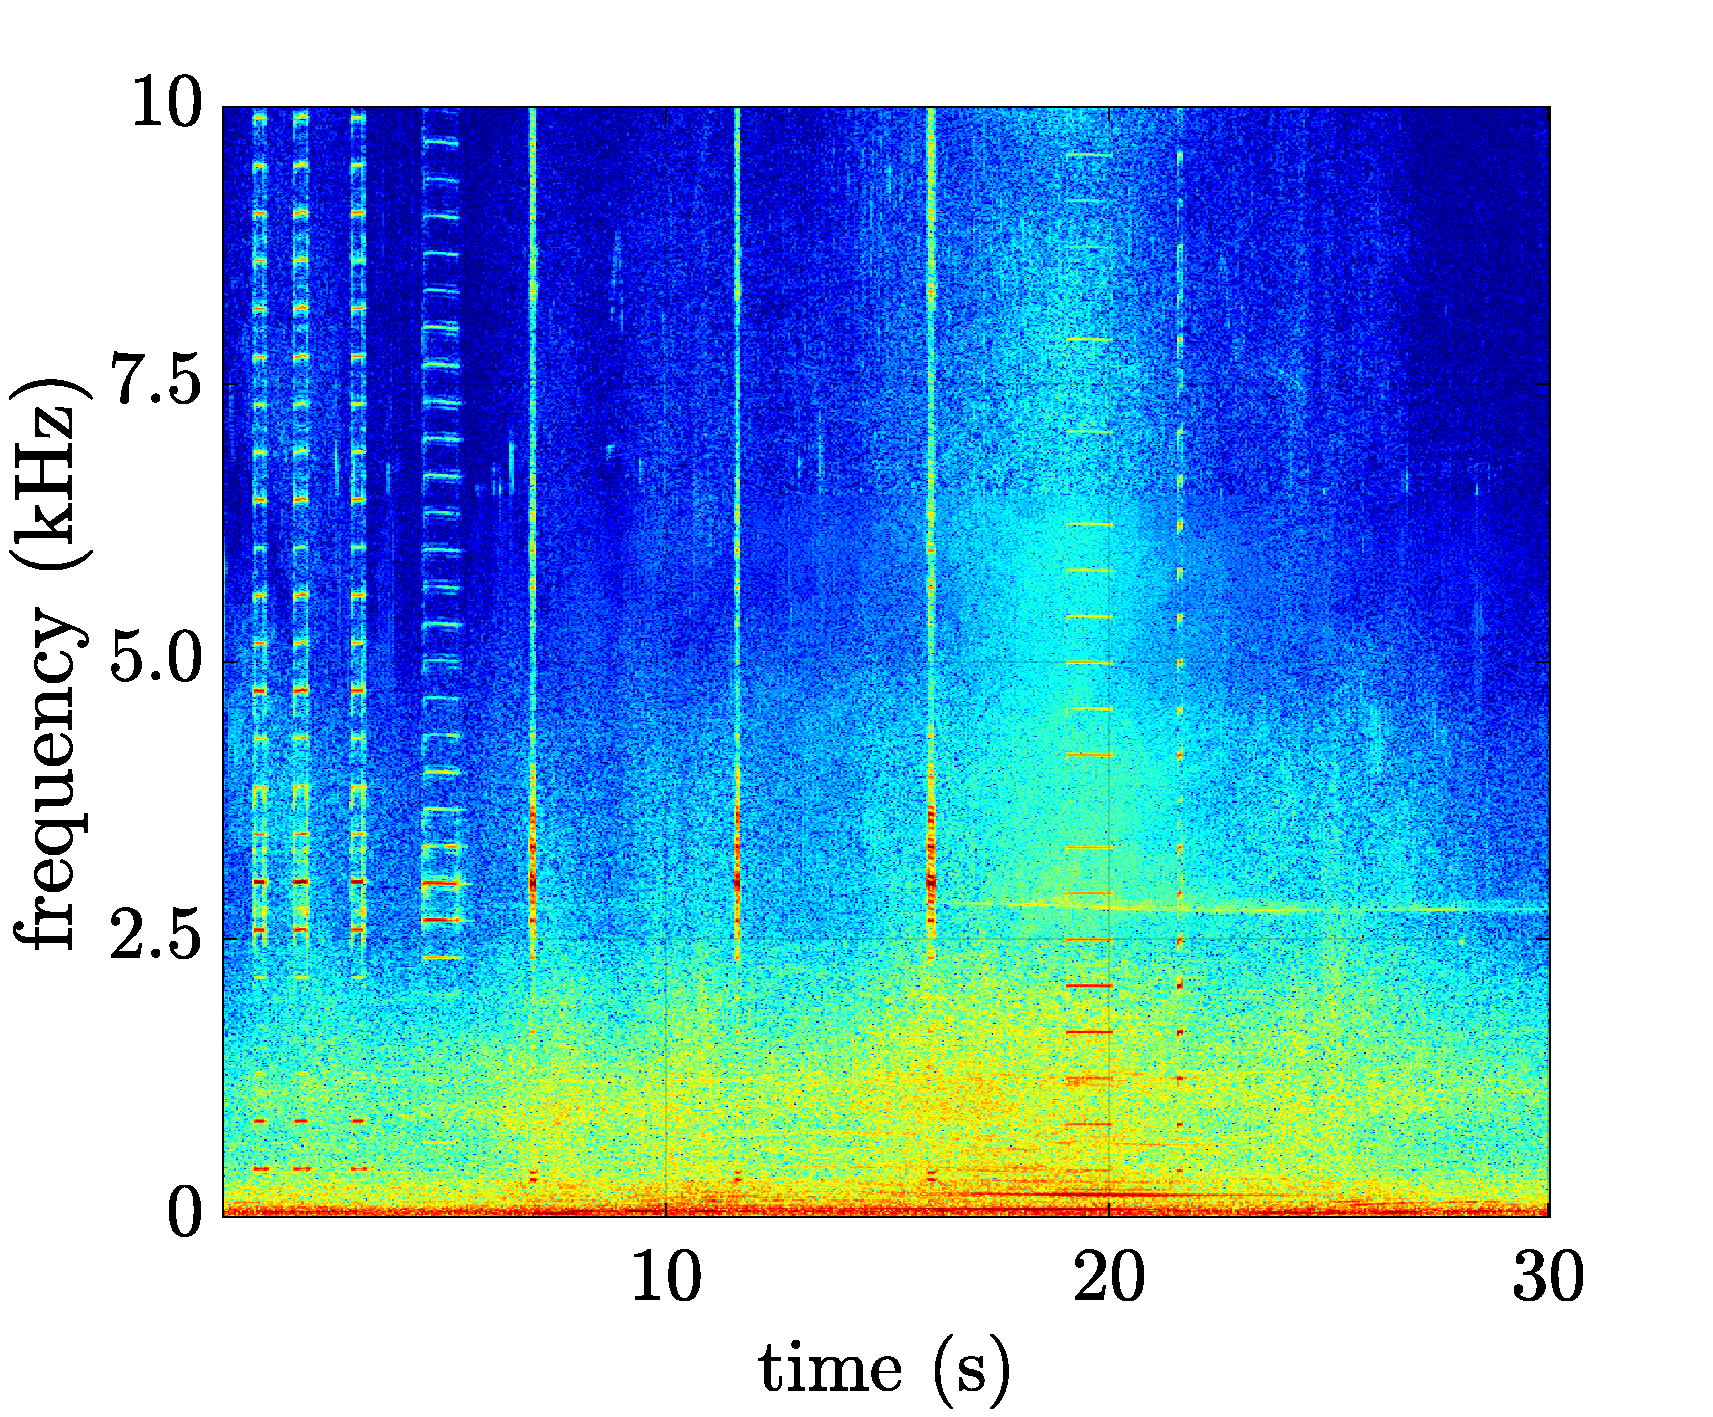
\includegraphics[width=.45\linewidth]{figures/specAlert.pdf}}
%DIF >   \hspace{5pt}
  \subfloat[]{\label{fig:lp_alert}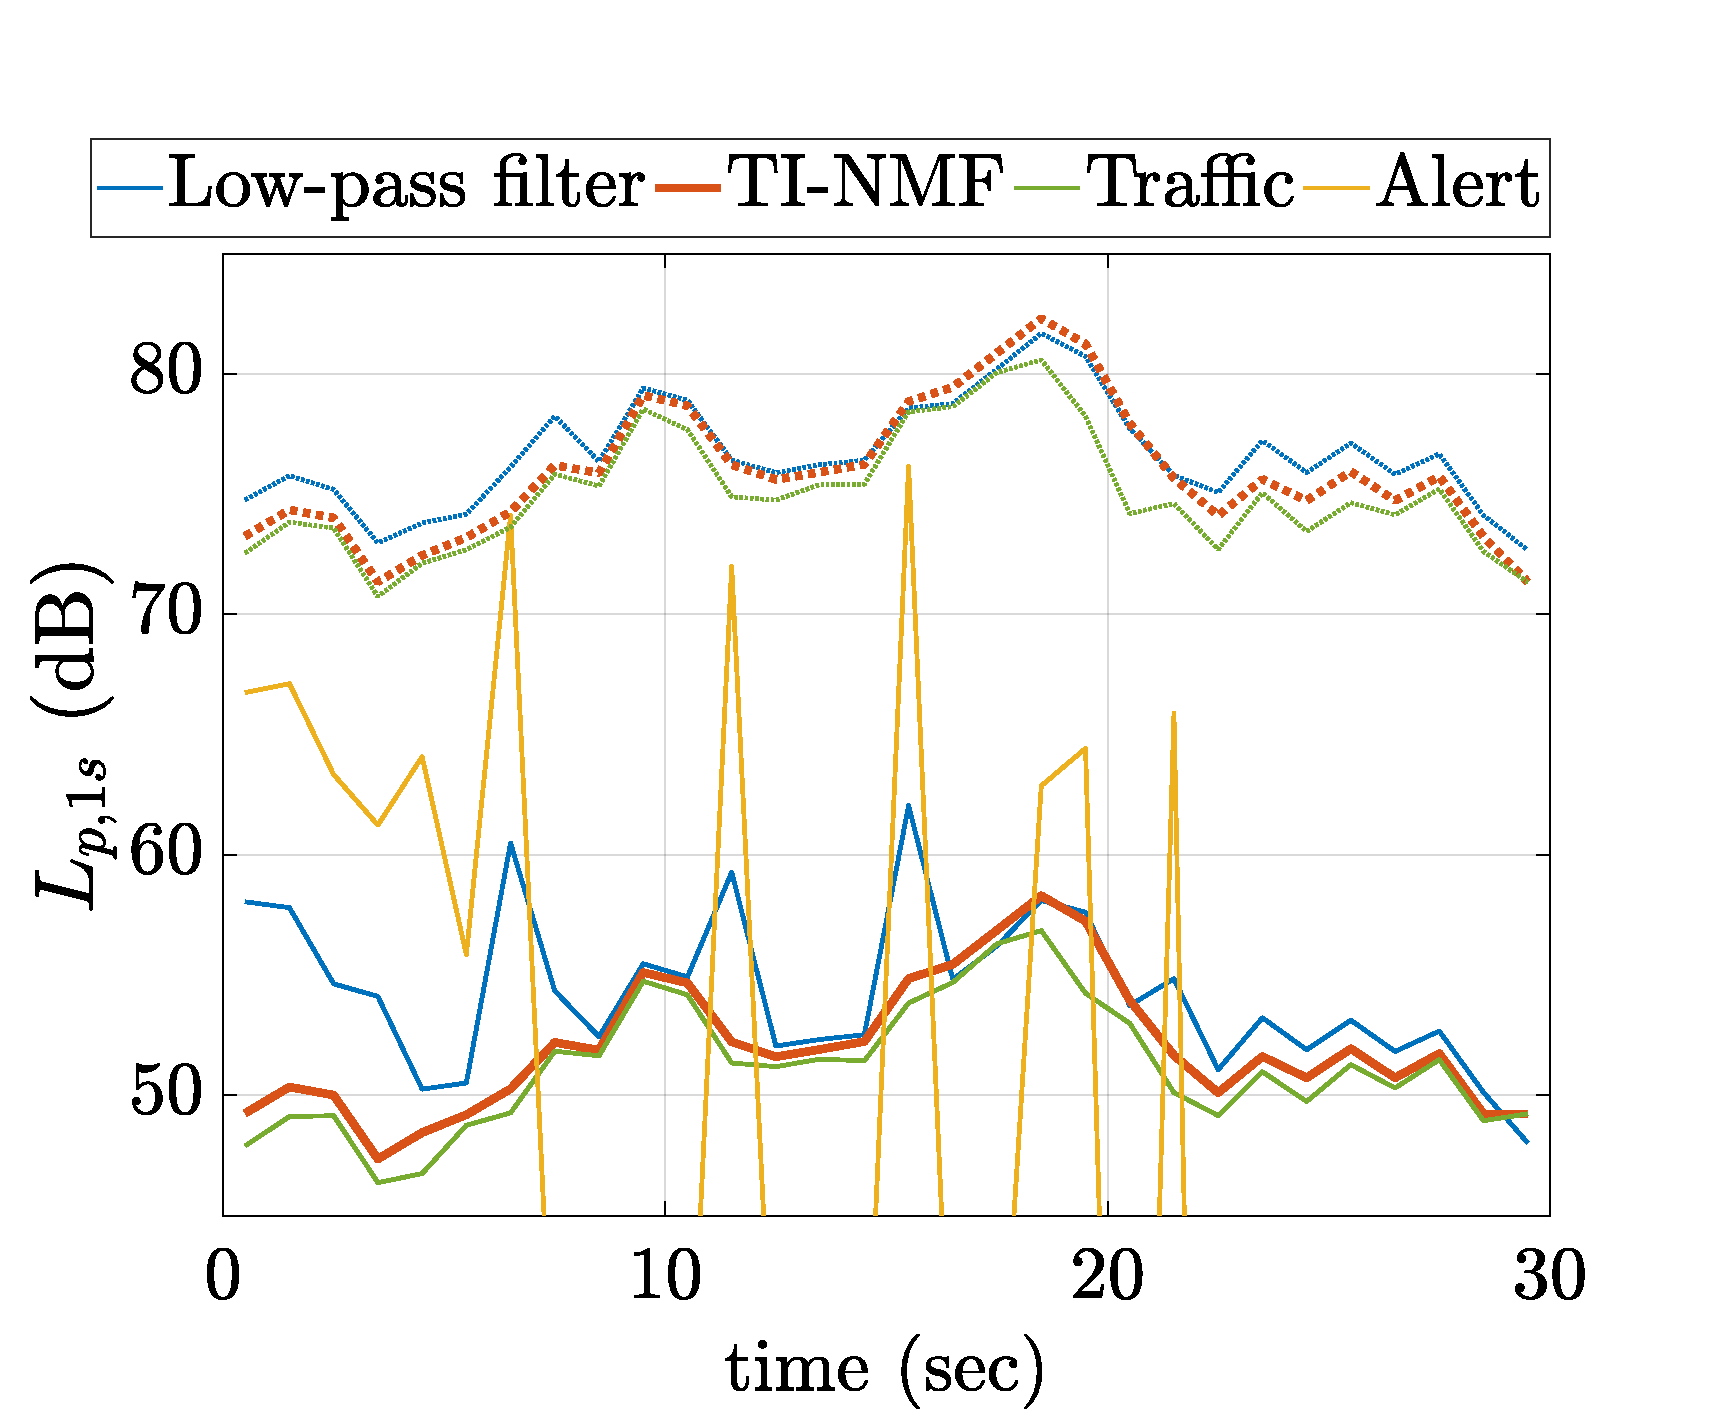
\includegraphics[width=.45\linewidth]{figures/NMF_Lp_alert.pdf}}
  \caption{\DIFaddFL{Spectrogram of an }\textit{\DIFaddFL{alert}} \DIFaddFL{sub-class scene (\ref{fig:specLp}) and evolution of 1 second equivalent sound pressure level (\ref{fig:lp_alert}) for 500 Hz low-pass filter and TI-NMF (\mbox{%DIFAUXCMD
$\beta$
}%DIFAUXCMD
= 1, \mbox{%DIFAUXCMD
$K$
}%DIFAUXCMD
= 200, \mbox{%DIFAUXCMD
$w_t$
}%DIFAUXCMD
= 0.5 s, \mbox{%DIFAUXCMD
$t$
}%DIFAUXCMD
= 0.42) at \mbox{%DIFAUXCMD
$TIR = -12$
}%DIFAUXCMD
dB (in full line) and \mbox{%DIFAUXCMD
$TIR$
}%DIFAUXCMD
= 12 dB (in dashed line).}}
  \label{fig:spec_alert}
\end{figure*}
\DIFaddend 

\section{Conclusion}

\DIFdelbegin \DIFdel{In this work the non negative metric factorization framework was used }\DIFdelend \DIFaddbegin \DIFadd{The non negative matrix factorization framework has been considered }\DIFaddend to estimate the road traffic sound level in urban sound mixtures. \DIFdelbegin \DIFdel{It }\DIFdelend \DIFaddbegin \DIFadd{We found that it }\DIFaddend is a well suited approach to these sound environments because it easily takes into account the overlap between the multiple sound sources present in the cities and it is adapted to monophonic sensor networks. Different versions of NMF have been studied as a supervised and semi-supervised approach. On a large corpus of sounds, the supervised approach proves to be too restrictive to be adapted to different sound environments whereas the semi-supervised approach has, on the contrary, too many degrees of freedom on the mobile dictionary $\mathbf{W_r}$, decreasing its performance especially when the traffic is predominant. The proposed approach, named threshold initialized NMF achieves the lowest average error \DIFaddbegin \DIFadd{on the entire corpus}\DIFaddend . With this method, the $\mathbf{W}$ is initialized with road traffic spectra, updated and the dictionary elements that are similar to the road traffic spectra are then extracted by hard thresholding.
\DIFaddbegin \DIFadd{The study of the error according each \mbox{%DIFAUXCMD
$TIR$
}%DIFAUXCMD
reveals that this method is not the most efficient on each \mbox{%DIFAUXCMD
$TIR$
}%DIFAUXCMD
. But it should be remind that one case, \mbox{%DIFAUXCMD
$TIR$
}%DIFAUXCMD
= -12 dB, is a rarer case than other values in an urban environment and is intended to test the performance limitations of the NMF TI. If this case was putted aside, TI-NMF reveals to be the only method to reach an \mbox{%DIFAUXCMD
$MAE$
}%DIFAUXCMD
error inferior  to 3 dB. The MAE error in Table 2 would decrease to 1.39 while SEM NMF would be 2.15 and the baseline would be 1.77. Consequently, for an urban application where the \mbox{%DIFAUXCMD
$TIR$
}%DIFAUXCMD
is an unknown information, TI NMF seems to be the most suited version. 
}\DIFaddend A major advantage of the proposed approach is that it is not designed for a specific source. \DIFdelbegin \DIFdel{Even though }\DIFdelend \DIFaddbegin \DIFadd{Extending the proposed approach to other sources is also of interest for future research. The method should thus be tested and validated further on a larger and more diverse dataset with, for instance, motorcycles and other noisy traffic elements which are not considered in this study. Furthermore, even if }\DIFaddend the experiments described in this paper focused on \DIFdelbegin \DIFdel{traffic sounds}\DIFdelend \DIFaddbegin \DIFadd{road traffic level detection}\DIFaddend , changing the dictionary to contain bird sounds would lead to an estimator of the presence of birds.
\DIFdelbegin \DIFdel{Extending the apporach to other sources is thus of intetrest for future research. Also, performance improvement could be achieved by the addition of constraints such as sparsness \mbox{%DIFAUXCMD
\cite{hoyer2004non} }%DIFAUXCMD
and smoothness \mbox{%DIFAUXCMD
\cite{virtanen_monaural_2007} }%DIFAUXCMD
of the low rank matrices.
}\DIFdelend 

The experimental protocol and the evaluated estimators have been implemented with the Matlab software. For reproducible purposes, the code is available online. The evaluation database composed of multiple samples of urban sounds is also made available for the research community with interest in detection, separation and recognition tasks of urban sound sources.

%\vspace{6pt}

\section*{Declarations}

\nomenclature{NMF}{Non-negative Matrix Factorization}
\nomenclature{Sup-NMF}{Supervised Non-negative Matrix Factorization}
\nomenclature{Sem-NMF}{Semi-Supervised Non-negative Matrix Factorization}
\nomenclature{TI-NMF}{Thresholded Initialized Non-negative Matrix Factorization}
\nomenclature{$TIR$}{Traffic Interfering Ratio}
\nomenclature{$\mathbf{V}$}{Magnitude spectrogram of the audio sample}
\nomenclature{$\mathbf{\tilde{V}}$}{Approximated spectrogram by the estimator}
\nomenclature{$\mathbf{\tilde{V}}_{traffic}$}{Approximated spectrogram of the traffic by the estimator}
\nomenclature{$\mathbf{V}_{f_c}$}{Approximated spectrogram resulting from the low-pass filter}
\nomenclature{$\mathbf{W}$}{Dictionary matrix}
\nomenclature{$\mathbf{H}$}{Activation matrix}
\nomenclature{$\mathbf{W_f}$}{$k$ element of the dictionary matrix}
\nomenclature{$\mathbf{W_s}$}{Fixed dictionary matrix for Sem-NMF}
\nomenclature{$\mathbf{W_r}$}{Mobile dictionary matrix for Sem-NMF}
\nomenclature{$\mathbf{H_s}$}{Activation matrix related $\mathbf{W_s}$ in Sem-NMF}
\nomenclature{$\mathbf{H_r}$}{Activation matrix for $\mathbf{W_r}$ in Sem-NMF}
\nomenclature{$\mathbf{W_0}$}{Initial dictionary matrix for TI-NMF}
\nomenclature{$\mathbf{W'}$}{Updated dictionary for TI-NMF}
\nomenclature{$MAE$}{Mean Absolute Error (dB)}
\nomenclature{$\mathbf{f_c}$}{Cut-off frequency (Hz)}
\nomenclature{$\mathbf{K}$}{Number of elements in $\mathbf{W}$}
\nomenclature{$\mathbf{w_t}$}{Rectangular window (second)}
\nomenclature{$\mathbf{t}$}{Threshold value}
\nomenclature{$\beta$}{Divergence class}
\printnomenclature

\section*{Availability of data and materials}
The dataset supporting the conclusions of this article is available in the \textit{urban$\_$traffic$\_$nmf$\_$dataset.zip}  repository,  \sloppy \burl{https://zenodo.org/record/1145855#.Wl2oPnkiGos}.
The software supporting the conclusions of this article is available in

 \begin{itemize} 
\item Project name: article2017EstimationAmbiance
\item \sloppy Project home page: \burl{https://github.com/jean-remyGloaguen/article2017EstimationAmbiance}
\item Archived version: \url{https://doi.org/10.5281/zenodo.1145855}
\item Programming language: Matlab
\item Other requirements: Matlab 2016b or higher
\item License: GNU GPL
\item Any restrictions to use by non-academics: license needed
 \end{itemize} 


\section*{Competing interests}
The authors declare that they have no competing interests.

\section*{Funding}
This study is co-funded by Ifsttar and Pays de la Loire region with a partial funding from the ANR under project reference ANR-16-CE22-0012.

\section*{Authors' contributions}
JG carried out the numerical \DIFdelbegin \DIFdel{experience }\DIFdelend \DIFaddbegin \DIFadd{experiment }\DIFaddend and drafted the manuscript. ML, AC and JP participated in the design of the study and helped to draft the manuscript.
All authors read and approved the final manuscript.

% \section*{Acknowledgements}

% BibTeX users please use one of
%\bibliographystyle{spbasic}      % basic style, author-year citations
\bibliographystyle{spmpsci}      % mathematics and physical sciences
%\bibliographystyle{spphys}       % APS-like style for physics
\bibliography{bibliographie_jasm}   % name your BibTeX data base


\end{document}
